%%%%%%%%%%%%%%%
%
% $Autor: Wings $
% $Datum: 2020-01-29 07:55:27Z $
% $Pfad: komponenten/Bilderkennung/Produktspezifikation/Nano33BLESense/Nano33BLESense.tex $
% $Version: 1785 $
%
% !TeX encoding = utf8
% !TeX root = Nano33BLESense
% !TeX TXS-program:bibliography = txs:///bibtex
%
%
%%%%%%%%%%%%%%%


% Auswahl der Sprache
% Die nicht gewünschte Sprache muss auskommentiert werden:
%\def\isGerman{1}
\def\isEnglish{1}



\documentclass[10pt,a4paper,bibliography=totoc]{scrbook}

%%%%%%%%%%%%%%%%%%%%%%%%%%%%%%
%
% $Autor: Wings $
% $Datum: 2020-01-30 07:43:10Z $
% $Pfad: komponenten/Bilderkennung/Produktspezifikation/JetsonNano/Allgemein/packages.tex $
% $Version: 1786 $
%
%
%%%%%%%%%%%%%%%%%%%%%%%%%%%%%%




\usepackage[left=4cm,right=4cm,top=2cm,bottom=2cm,includeheadfoot]{geometry}
\setlength{\headheight}{1pt}

% Standard Deutsch
\usepackage{lmodern}
\usepackage[utf8]{inputenc}
\ifdefined\isGerman
  \usepackage[ngerman]{babel}
\else
  \ifdefined\isEnglish
    \usepackage[english]{babel}
  \else
    \usepackage[ngerman]{babel}
  \fi
\fi

\usepackage[T1]{fontenc}

% Farben
\usepackage{xcolor}
\usepackage{alltt}
% Notwendig für Syntax-Highlighting mit besonderen Farben
%\usepackage[table, x11names]{xcolor}


% Pakete für Mathe
\usepackage{amsmath}
\usepackage{amsfonts}
\usepackage{amssymb}
\usepackage{mathtools}


% Paket Internetrefferenzen
\usepackage{hyperref}

%Wird zusätzlich das Paket showidx eingebunden, werden die gesetzten Einträge am Seitenrand dargestellt. 
\usepackage{imakeidx}
%\usepackage{showidx}
%\usepackage[override=false]{seealso}
\makeindex[intoc,title=Index]
\ifdefined\isGerman
  \renewcommand{\indexname}{Stichwortverzeichnis}
\else
\ifdefined\isEnglish
\else
  \renewcommand{\indexname}{Stichwortverzeichnis}
\fi
\fi




% Paktete für Bilder
\usepackage{graphicx}

\usepackage{listings}
% Automatische erstellung von Referenzen
\usepackage[ngerman]{cleveref}
% Zeilenumbrüche in \texttt
\usepackage[htt]{hyphenat}

% Automatisches erstellen und referenzieren eines Abkürzungsverzeichnisses
\usepackage[tooltip]{acro}
% Ermöglicht Verwendung von 'H' Float modifier
\usepackage{float}

% Ermöglicht Subfigures und Subcaptions
\usepackage{subcaption}


\usepackage{float}
\usepackage{array}
\usepackage{amsopn}
\usepackage[percent]{overpic}
\usepackage{colortbl}
\usepackage{marginnote}

\usepackage{textcomp}

\usepackage[
backend=bibtex8,%  defernumbers=true,
autocite=inline,
labelalpha=true,%  sorting=none,
firstinits=true,
uniquename=init,
uniquelist=false,
refsegment=section,
style=alphabetic,
safeinputenc
]{biblatex}

%\usepackage[german]{babelbib}
%\usepackage[square,sort,comma,numbers]{natbib}
%\DeclareNameAlias{sortname}{last-first}
%\bibliographystyle{geralpha}
%\setcitestyle{square,aysep={},yysep={;}}
%\newcommand*{\multicitedelim}{\addsemicolon\space}


% Verwendung:
%\Ausblenden{.....
%} %todo Ausblenden



% Kapitel entfernen
%\usepackage{titlesec}

\usepackage{tabularx} 
\usepackage{longtable}
\usepackage{framed}
\usepackage{tocbibind}

\usepackage[official]{eurosym}

\usepackage{listings}
\definecolor{mygreen}{rgb}{0,0.6,0}
\definecolor{mygray}{rgb}{0.5,0.5,0.5}
\definecolor{mymauve}{rgb}{0.58,0,0.82}

\lstset{ 
  backgroundcolor=\color{white},   % choose the background color; you must add \usepackage{color} or \usepackage{xcolor}; should come as last argument
  basicstyle=\footnotesize,        % the size of the fonts that are used for the code
  breakatwhitespace=false,         % sets if automatic breaks should only happen at whitespace
  breaklines=true,                 % sets automatic line breaking
  captionpos=b,                    % sets the caption-position to bottom
  commentstyle=\color{mygreen},    % comment style
  deletekeywords={...},            % if you want to delete keywords from the given language
  escapeinside={\%*}{*)},          % if you want to add LaTeX within your code
  extendedchars=true,              % lets you use non-ASCII characters; for 8-bits encodings only, does not work with UTF-8
  firstnumber=1000,                % start line enumeration with line 1000
  frame=single,	                   % adds a frame around the code
  keepspaces=true,                 % keeps spaces in text, useful for keeping indentation of code (possibly needs columns=flexible)
  keywordstyle=\color{blue},       % keyword style
  language=Python,                 % the language of the code
  morekeywords={*,...},            % if you want to add more keywords to the set
  numbers=left,                    % where to put the line-numbers; possible values are (none, left, right)
  numbersep=5pt,                   % how far the line-numbers are from the code
  numberstyle=\tiny\color{mygray}, % the style that is used for the line-numbers
  rulecolor=\color{black},         % if not set, the frame-color may be changed on line-breaks within not-black text (e.g. comments (green here))
  showspaces=false,                % show spaces everywhere adding particular underscores; it overrides 'showstringspaces'
  showstringspaces=false,          % underline spaces within strings only
  showtabs=false,                  % show tabs within strings adding particular underscores
  stepnumber=2,                    % the step between two line-numbers. If it's 1, each line will be numbered
  stringstyle=\color{mymauve},     % string literal style
  tabsize=2,	                   % sets default tabsize to 2 spaces
  title=\lstname                   % show the filename of files included with \lstinputlisting; also try caption instead of title
} 
\lstset{language=Python}




\pagestyle{empty}




% Kopfzeile
\usepackage{fancyhdr}
\pagestyle{fancy}
\fancyhf{}
\fancyhead[OL]{\nouppercase{\leftmark}}
\fancyhead[OR]{\thepage}
\fancyhead[ER]{\nouppercase{\leftmark}}
\fancyhead[ER]{\nouppercase{\chaptermark{}}}
\fancyhead[ER]{\nouppercase{\chaptermark{}}}
\fancyhead[EL]{\thepage}
\renewcommand{\headrulewidth}{0.1pt} 



%\AtBeginDocument{\renewcommand{\chaptername}{}} % muss nach babel stehen! 



\usepackage{ifthen}

\usepackage{media9}
\usepackage{animate}
\newcounter{AnimateAngle}
\setcounter{AnimateAngle}{0}
\newcounter{AnimateStepFactor}
\setcounter{AnimateStepFactor}{1}
\newcounter{AnimateSteps}
\setcounter{AnimateSteps}{0}


\usepackage{multirow}                  % Tabelle vertikale Zellen verbinden
\usepackage{rotating}                  % text rotieren \rotatebox{90}{text}
\usepackage{colortbl}                  % Farbe der Zellen einer Tabelle, z. B. \begin{tabular}{c>{\columncolor{green}}cc}

\usepackage{enumitem}
\usepackage{spverbatim}

% Korrekte darstellung von SI-Einheiten
\usepackage[binary-units=true, per-mode=symbol]{siunitx}
% Erstellen einer ToDo-Liste
\usepackage[ngerman, colorinlistoftodos]{todonotes}
% Kommando zum markieren fehlender praktischer Umsetzungen
\newcommand{\todop}[2][]{\todo[color=red, inline, #1]{#2}}
\usepackage{makecell}
% Bera Mono als \ttfamily font
\usepackage[scaled]{beramono}

\usepackage{menukeys}
\usepackage{textcomp}


% Add section names to todonotes list
\makeatletter
\let\ori@chapter\@chapter
\def\@chapter[#1]#2{\ori@chapter[#1]{#2}%
    \if@mainmatter\addcontentsline{tdo}{chapter}{\protect\numberline{\thechapter}{#1}}%
    \else\addcontentsline{tdo}{chapter}{#1}%
    \fi}
\makeatother

% Farben für Syntax-Highlighting
\definecolor{dkgreen}{rgb}{0,.6,0}
\definecolor{dkblue}{rgb}{0.655,0.113,.364}
\definecolor{dkyellow}{cmyk}{0,0,.8,.3}

\definecolor{parameterc}{rgb}{.4,0,.6}
\definecolor{typec}{rgb}{0,0.525,.702}
\definecolor{stringc}{rgb}{0,.5019,.5019}
\definecolor{keywordc}{rgb}{.6549, .1137, .3647}
\definecolor{commentc}{rgb}{.5882, .5960, .5882}
\definecolor{textc}{rgb}{.2,.2,.2}

\lstdefinestyle{all}{
    alsoletter={-},
    frame=single, 	% top,frame=bottom,
    numbers=none,
    numberstyle=\tiny\color{textc},
    basicstyle=\linespread{0.9}\ttfamily\footnotesize\color{textc},
    tabsize=4,
    showstringspaces=false,
    captionpos=t,
    rulecolor=\color{lightgray!40},
    keywordstyle=\color{keywordc},
    stringstyle=\color{stringc},
    commentstyle=\color{commentc},
    breaklines=true,
    escapechar="!",
    postbreak=\mbox{\textcolor{green}{$\hookrightarrow$}\space},
}

\lstdefinestyle{bashstyle}{
    style=all,
    keywords=[2]{-y, --no-install-recommends, --allow-change-held-packages, --allow-downgrades, --fetch-keys, -n, --version, --params, -c, -i, -O, --upgrade, --no-cache-dir, --extra-index-url, --show, -s, -m},
    keywordstyle=[2]\color{parameterc},
    morekeywords = {ln,choco,pip,pip3,apt,apt-key,apt-get,apt-mark,add-apt-repository,wget,mktemp,dpkg,dpkg-query,echo,>>,rm,tegrastats, systemctl},
    deletekeywords={local,LOCAL},
}

\lstdefinestyle{pythonstyle}{
    style=all,
    morekeywords={as},
    keywords=[2]{True, False, None},
    keywordstyle=[2]\color{typec},
    alsoletter={_},
    keywords=[3]{max_workspace_size_bytes, precision_mode, maximum_cached_engines, use_calibration, optimizer, loss, input_shape, from_logits, metrics, batch_size, epochs, validation_data, activation, use_calibration, filters, kernel_size, pool_size, units},
    keywordstyle=[3]\color{parameterc},
    deletekeywords={compile,COMPILE},
}

\lstdefinestyle{inlinestyle}{
    style=all,
    breaklines        = true,
    breakatwhitespace = true,
    breakindent       = 2ex,
    escapechar        = *,
    numbers           = left,
    postbreak=,
}
\lstdefinelanguage{MyBash} {
    language = Bash,
    style=bashstyle,
}

\lstdefinelanguage{MyPython} {
    language = Python,
    style=pythonstyle,
}


%%%%%%%%%%%%%%%%%%%%%%%%%%%%%%
%
% $Autor: Wings $
% $Datum: 2020-01-24 14:19:22Z $
% $Pfad: komponenten/Bilderkennung/Produktspezifikation/JetsonNano/Allgemein/commands.tex $
% $Version: 1782 $
%
%
%%%%%%%%%%%%%%%%%%%%%%%%%%%%%%




%\titleformat{\chapter}{\bfseries\Huge}{\thechapter.\quad}{0em}{}

\renewcommand{\indexname}{Stichwortverzeichnis}


\DeclareMathOperator{\Atan2}{Atan2}
\DeclareMathOperator{\sign}{sign}
\DeclareMathOperator{\ReLU}{ReLU}

%Zahlenmengen
\newcommand{\C}{\mathbb{C}}
\newcommand{\R}{\mathbb{R}}
\newcommand{\N}{\mathbb{N}}
\newcommand{\Z}{\mathbb{Z}}
\newcommand{\Q}{\mathbb{Q}}
\newcommand{\Po}{\mathbb{P}}
\newcommand{\Rp}[2]{\mathbb{R}^{[#1;\,#2]}} % Menge der auf [a,b]-periodischen Funktionrn
%\DeclareMathOperator{\arg}{arg}

\newcommand*\justify{%
	\fontdimen2\font=0.4em% interword space
	\fontdimen3\font=0.2em% interword stretch
	\fontdimen4\font=0.1em% interword shrink
	\fontdimen7\font=0.1em% extra space
	\hyphenchar\font=`\-% allowing hyphenation
}


\newcommand{\MyComplex}[1]{\mathbf{#1}}
\newcommand{\Laplaceinv}[1]{#1}
\newcommand{\MapleCommand}[1]{\textcolor{MapleColor}{\texttt{\justify#1}}}
\newcommand{\PYTHON}[1]{\textcolor{PythonColor}{\texttt{\justify#1}}}
\newcommand{\SHELL}[1]{\textcolor{ShellColor}{\texttt{\justify#1}}}
\newcommand{\FILE}[1]{\textcolor{FileColor}{\texttt{\justify#1}}}
\newcommand{\Bez}{Bézier}
\newcommand{\PH}{pythagoreische Hodographen \xspace}
\newcommand{\PHd}{pythagoreischen Hodographen \xspace}





\setlength{\parindent}{0pt}




\definecolor{uuuuuu}{rgb}{0.26666666666666666,0.2666666666666666,0.26666666666666666}
\definecolor{qqqqff}{rgb}{0.,0.,1.}
\definecolor{MapleColor}{rgb}{1,0.5,0.}
\definecolor{PythonColor}{rgb}{0,0.5,1.}
\definecolor{ShellColor}{rgb}{1,0,0.5}
\definecolor{FileColor}{rgb}{0.5,0.5,1.}

\definecolor{LightGoldenrod}{rgb}{0.8,.9,0.3} 
\definecolor{AliceBlue}{rgb}{0.5,.8,1}
\definecolor{LightGrey}{rgb}{0.9,0.9,0.9} 
\definecolor{Beige}{rgb}{0.9,0.5,0.0} 
\definecolor{Gelb}{rgb}{0.999,0.999,0.0} 


\definecolor{LightCyan}{rgb}{0.88,1,1}
\definecolor{frenchblue}{rgb}{0.0, 0.45, 0.73}
\definecolor{greenblue}{rgb}{0.0, 0.25, 0.3}
\definecolor{darkcyan}{rgb}{0.0, 0.55, 0.55}
\definecolor{bondiblue}{rgb}{0.0, 0.58, 0.71}
\definecolor{grayleft}{rgb}{0.1, 0.1, 0.1}
\definecolor{grayright}{rgb}{0.2, 0.2, 0.2}
\definecolor{graycircle}{rgb}{0.3, 0.3, 0.3}
\definecolor{graylight}{rgb}{0.8, 0.8, 0.8}
\definecolor{greenenglish}{rgb}{0.0, 0.5, 0.0}
\definecolor{darkpastelgreen}{rgb}{0.01, 0.75, 0.24}
\definecolor{copper}{rgb}{0.72, 0.45, 0.2}
\definecolor{greenyellow}{rgb}{0.68, 1.0, 0.18}
\definecolor{fuchsia}{rgb}{1.0, 0.0, 1.0}
\definecolor{silver}{rgb}{0.75, 0.75, 0.75}
\definecolor{deepskyblue}{rgb}{0.0, 0.75, 1.0}


\newcommand{\GND}{\cellcolor{black}\textcolor{white}{GND}}
\newcommand{\Vf}{\cellcolor{red}\textcolor{black}{5V}}
\newcommand{\Vd}{\cellcolor{red}\textcolor{black}{3.3V}}
\definecolor{LightCyan}{rgb}{0.88,1,1}

\newcolumntype{a}{>{\columncolor{LightCyan}}c}


\newcounter{FortlaufendeNummer}
\setcounter{FortlaufendeNummer}{1}
\newcounter{LetztesKapitel}
\setcounter{LetztesKapitel}{-1}

\newcounter{BeamerChapter}
\setcounter{BeamerChapter}{1}


\graphicspath{%
	{../Bilder/},{Bilder/},{../../Bilder/},%
	{../../../../Allgemeines/},{../../../Allgemeines/},{../../Allgemeines/},%
	{../../../../Aufgaben/},{../../../Aufgaben/},%
	{../}}

\newcommand{\GRAPHICSC}[3]{\begin{center}
		\includegraphics[scale=#1]{#3}
\end{center}}

\newcommand{\GRAPHICS}[3]{\includegraphics[scale=#1]{#3}}

\newcommand{\FONO}{   
%\ifthenelse{\value{chapter} > \value{LetztesKapitel}}%
%{%
%\setcounter{LetztesKapitel}{\value{chapter}}%
%\setcounter{FortlaufendeNummer}{1}%
%}%
%\arabic{chapter}.\arabic{FortlaufendeNummer}.%
%\stepcounter{FortlaufendeNummer}%
}

\newcommand{\FONOBEAMER}{%
\ifthenelse{\value{BeamerChapter}>0}%
{%
  \ifthenelse{\value{BeamerChapter}>\value{LetztesKapitel}}%
  {%
    \setcounter{LetztesKapitel}{\value{BeamerChapter}}%
    \setcounter{FortlaufendeNummer}{1}%
}%
\hbox{}\arabic{BeamerChapter}.\arabic{FortlaufendeNummer}.\stepcounter{FortlaufendeNummer}%
}%
\hbox{}%
} 


\newcommand{\FONOBEAMERSTEP}{%
\ifthenelse{\value{BeamerChapter}>0}%
{%
  \ifthenelse{\value{BeamerChapter}>\value{LetztesKapitel}}%
  {%
    \setcounter{LetztesKapitel}{\value{BeamerChapter}}%
    \setcounter{FortlaufendeNummer}{1}%
}%
\stepcounter{FortlaufendeNummer}%
}%
\hbox{}%
\bigskip
} 

\newcommand{\FONOBEAMERSTAY}{   
\ifthenelse{\value{BeamerChapter}>\value{LetztesKapitel}}
{
\setcounter{LetztesKapitel}{\value{BeamerChapter}}
\setcounter{FortlaufendeNummer}{1}
}
\hbox{}\arabic{BeamerChapter}.\arabic{FortlaufendeNummer}.} 


% \FONOBEAMERSTEP
% \SATZNAME{}{}
% \SATZ{}
% \SATZNAMES{}{}
% \SATZS{}
% \STANDARD{}{}
% \STANDARDN{}{}  handout:0
% \STANDARDV{}{}  verbatim
% \DEF{}
% \DEFNAME{}{}
% \DEFS{}
% \DEFNAMES{}{}
% \BEMERKUNG{}
% \BEMERKUNGNAME{}{}
% \BEMERKUNGNAMES{}{}
% \BEISPIELNAME{}{}
% \BEISPIELNAMES{}{}
% \BEISPIEL{}
% \BEISPIELS{}



\newcommand{\Def}[1]
{
   \definecolor{shadecolor}{rgb}{0.98, 0.91, 0.71}

   \begin{snugshade*}
         \textbf{\FONOBEAMER  Definition.} #1
    \end{snugshade*}

    \bigskip
}

\newcommand{\DefN}[2]
{
   \definecolor{shadecolor}{rgb}{0.98, 0.91, 0.71}

   \begin{snugshade*}
         \textbf{ \FONOBEAMER Definition #1.}  #2
    \end{snugshade*}

    \bigskip
}


\newcommand{\Satz}[1]
{
   \definecolor{shadecolor}{rgb}{0.74, 0.83, 0.9}

   \begin{snugshade*}
         \textbf{\FONOBEAMER  Satz.} #1
    \end{snugshade*}

    \bigskip
}

\newcommand{\SatzN}[2]
{
   \definecolor{shadecolor}{rgb}{0.74, 0.83, 0.9}

   \begin{snugshade*}
         \textbf{ \FONOBEAMER Satz #1.}  #2
    \end{snugshade*}

    \bigskip
}

\newcommand{\Bemerkung}[1]
{
   \definecolor{shadecolor}{rgb}{0.66, 0.89, 0.63}

   \begin{snugshade*}
         \textbf{\FONOBEAMER  Bemerkung.} #1
    \end{snugshade*}

    \bigskip
}

\newcommand{\BemerkungN}[2]
{
   \definecolor{shadecolor}{rgb}{0.66, 0.89, 0.63} %Lavendel

   \begin{snugshade*}
         \textbf{ \FONOBEAMER Bemerkung #1.}  #2
    \end{snugshade*}

    \bigskip
}


\newcommand{\Beispiel}[1]
{
   \definecolor{shadecolor}{rgb}{0.9, 0.9, 0.98} 

   \begin{snugshade*}
         \textbf{\FONOBEAMER  Beispiel.} #1
    \end{snugshade*}

    \bigskip
}

\newcommand{\BeispielN}[2]
{
   \definecolor{shadecolor}{rgb}{0.9, 0.9, 0.98} 

   \begin{snugshade*}
         \textbf{ \FONOBEAMER Beispiel #1.}  #2
    \end{snugshade*}

    \bigskip
}


%todo Die Kommandos sind für das Endprodukt zu entfernen. Die entsprechenden Stellen sind zu bearbeiten bzw. zu löschen
\newcommand{\Mynote}[1]{\marginnote{\textcolor{red}{WS:#1}}}
\newcommand{\Ausblenden}[1]{}
\newcommand{\ToDo}[1]{\textcolor{red}{\section{ToDo} #1}}


\newcommand{\GRAFIKEINFUEGEN}{\textcolor{red}%
{\bf Hier ist eine Grafik einzufügen}}
\newcommand{\QUELLE}{\textcolor{red}{\bf Hier ist eine Quelle einzufügen}}
\newcommand{\neu}{\textcolor{red}{Wort Einfügen}}
\newcommand{\REFERENZ}{\textcolor{red}%
{\bf Referenz  einzufügen}}
\newcommand{\EXAMPLE}{\textcolor{red}%
{\bf Beispiel einzufügen}}


%
%\newcommand{\STANDARD}[1]{#1}
%\newcommand{\STANDARDN}[1]{#1}
%\newcommand{\beamergotobutton}[1]{#1}
%\newcommand{\MysectionZ}[2]{#2}
%
\newcommand{\trinom}[3]{\left(\begin{array}{c} #1\\#2\\#3 \\ \end{array}\right)}


\newcommand{\textdirectcurrent}{%
	\settowidth{\dimen0}{$=$}%
	\vbox to .85ex {\offinterlineskip
		\hbox to \dimen0{\leaders\hrule\hfill}
		\vskip.35ex
		\hbox to \dimen0{%
			\leaders\hrule\hskip.2\dimen0\hfill
			\leaders\hrule\hskip.2\dimen0\hfill
			\leaders\hrule\hskip.2\dimen0
		}
		\vfill
	}%
}
\newcommand{\mathdirectcurrent}{\mathrel{\textdirectcurrent}}

\newlist{notes}{enumerate}{1}
\setlist[notes]{label=Note: ,leftmargin=*}


% Kommandos für In-Line Code
\newcommand{\COMMAND}[1]{\lstinline[language=MyBash, style=inlinestyle]{#1}}
\newcommand{\mytt}[1]{\texttt{\footnotesize #1}}
\newcommand{\python}[1]{\lstinline[language=MyPython, style=inlinestyle]{#1}}
\newcommand{\twod}[2]{
    \ensuremath{{#1} \times {#2}}}
\newcommand{\threed}[3]{
    \ensuremath{{#1} \times {#2} \times {#3}}}

% Fett-geschriebene Tabellenberschriften
\renewcommand\theadfont{\bfseries}


\newcommand{\us}{\si{\micro\second}}
\newcommand{\usn}[1]{\SI{#1}{\micro\second}}
\renewcommand{\textapprox}{\raisebox{0.5ex}{\texttildelow}}

% Auswahl der Sprache
% 1.Argument ist der Pfad ohne "en" oder "de"
% 2.Argument ist der Dateiname
\newcommand{\InputLanguage}[2]{
\ifdefined\isGerman
  \input{#1de/#2}
\else
  \ifdefined\isEnglish
   \input{#1en/#2}
  \else
	\input{#1de/#2}
  \fi
\fi
}

\newcommand{\TRANS}[2]{%
	\ifdefined\isGerman	
	  #1	
	\else 
	  \ifdefined\isEnglish 
	    #2 
	  \else	
	    #1 
	  \fi 
	\fi
}
\renewcommand{\TRANS}[2]{#1}



\DeclareCaptionType{code}[Listing][Liste des Listings] 
%%%%%%%%%%%%%%%%%%%%%%%%%%%%%%
%
% $Autor: Wings $
% $Datum: 2019-12-09 11:50:02Z $
% $Pfad: komponenten/Bilderkennung/Produktspezifikation/CorelTPU/TPU/Allgemein/tikzdefs.tex $
% $Version: 1766 $
%
%
%%%%%%%%%%%%%%%%%%%%%%%%%%%%%%


% Definition für tikz

\usepackage{pgfplots}
\usepackage{pgf,tikz}
\usepackage{mathrsfs}
\usepackage{tikz}
\usetikzlibrary{shapes,shapes.symbols,shapes.misc, shapes.multipart, shapes.geometric,arrows,angles,quotes,babel,positioning,calc,math,matrix}

\usetikzlibrary{positioning,fadings,through}


\usepackage{tikz-3dplot}

\tikzset{
  input2/.style={ % requires library shapes.geometric
    draw,
    trapezium,
    trapezium left angle=60,
    trapezium right angle=120,
  },
  process rectangle outer width/.initial=0.15cm,
  predefined process/.style={
    rectangle,
    draw,
    append after command={
      \pgfextra{
        \draw [fill=blue!20]
        ($(\tikzlastnode.north west)-(0,0.5\pgflinewidth)$)--
        ($(\tikzlastnode.north west)-(\pgfkeysvalueof{/tikz/process rectangle outer width},0.5\pgflinewidth)$)--
        ($(\tikzlastnode.south west)+(-\pgfkeysvalueof{/tikz/process rectangle outer width},+0.5\pgflinewidth)$)--
        ($(\tikzlastnode.south west)+(0,0.5\pgflinewidth)$);
        \draw [fill=blue!20]
        ($(\tikzlastnode.north east)-(0,0.5\pgflinewidth)$)--
        ($(\tikzlastnode.north east)+(\pgfkeysvalueof{/tikz/process rectangle outer width},-0.5\pgflinewidth)$)--
        ($(\tikzlastnode.south east)+(\pgfkeysvalueof{/tikz/process rectangle outer width},0.5\pgflinewidth)$)--
        ($(\tikzlastnode.south east)+(0,0.5\pgflinewidth)$);
      }  
    },
    text width=#1,
    align=center, fill=blue!20,  minimum height=4em
  },
  predefined process/.default=20mm,
  data1/.style={
    trapezium, 
    trapezium left angle=70, 
    trapezium right angle=110, 
    text width=1.5cm, 
    inner ysep=17pt,
    align=center, 
    line width=2pt,
    fill=blue!20
  },      
}


%Kabinettprojektion von 3D auf 2D
%
% Eingabe
% x,y,z
%
% Ausgabe
% x- oder y-Wert des Punkts
\newcommand{\Proj}[3]{({#1-#3*0.5*cos(30)},{#2-#3*0.5*sin(30)})}
\tikzset{declare function={ProjX(\x,\y,\z)=\x-\z*0.5*cos(30);}}
\tikzset{declare function={ProjY(\x,\y,\z)=\y-\z*0.5*sin(30);}}

%Rotation um die x-Achse 
%
% Eingabe
% x,y,z,alpha
%
% Ausgabe
% 
% x-, y- oder z-Wert des Punkts
\tikzset{declare function={RotXx(\x,\y,\z,\a)=\x;}}
\tikzset{declare function={RotXy(\x,\y,\z,\a)=\y*cos(\a)-\z*sin(\a);}}
\tikzset{declare function={RotXz(\x,\y,\z,\a)=\y*sin(\a)+\z*cos(\a);}}


%Rotation um die y-Achse 
%
% Eingabe
% x,y,z,alpha
%
% Ausgabe
% 
% x-, y- oder z-Wert des Punkts
\tikzset{declare function={RotYx(\x,\y,\z,\a)=\x*cos(\a)-\z*sin(\a);}}
\tikzset{declare function={RotYy(\x,\y,\z,\a)=\y;}}
\tikzset{declare function={RotYz(\x,\y,\z,\a)=\x*sin(\a)+\z*cos(\a);}}



%Rotation um die z-Achse 
%
% Eingabe
% x,y,z,alpha
%
% Ausgabe
% 
% x-, y- oder z-Wert des Punkts
\tikzset{declare function={RotZx(\x,\y,\z,\a)=\x*cos(\a)-\y*sin(\a);}}
\tikzset{declare function={RotZy(\x,\y,\z,\a)=\x*sin(\a)+\y*cos(\a);}}
\tikzset{declare function={RotZz(\x,\y,\z,\a)=\z;}}


%Rotation um die x-Achse 
%
% Eingabe
% x,y,z,alpha
%
% Ausgabe
% Punkt {x}{y}{z}
\newcommand{\RotXx}[4]{#1}%
\newcommand{\RotXy}[4]{(cos(#4)*#2-sin(#4)*#3)}
\newcommand{\RotXz}[4]{(sin(#4)*#2+cos(#4)*#3)}%


\tikzset{declare function={bellshape(\x,\mu,\sigma)=exp(-(\x-\mu)^2/(2*\sigma^2));}}


%Rotation um die x-Achse mit Projektion
%
% Eingabe
% x,y,z,alpha
%
% Ausgabe
% Punkt ({x}, {y})
\newcommand{\RotXP}[4]%
{(%
{#1-(sin(#4)*#2+cos(#4)*#3)*0.5*cos(30)},%
{cos(#4)*#2-sin(#4)*#3-(sin(#4)*#2+cos(#4)*#3)*0.5*sin(30)})%
}

%Rotation um die y-Achse mit Projektion
%
% Eingabe
% x,y,z,alpha
%
% Ausgabe
% Punkt ({x}, {y})
\newcommand{\RotYP}[4]%
{(%
{cos(#4)*#1+sin(#4)*#3-(-sin(#4)*#1+cos(#4)*#3)*0.5*cos(30)},%
{#2-(-sin(#4)*#1+cos(#4)*#3)*0.5*sin(30)}%
)}


%Rotation um die z-Achse mit Projektion
%
% Eingabe
% x,y,z,alpha
%
% Ausgabe
% Punkt ({x}, {y})
\newcommand{\RotZP}[4]%
{({cos(#4)*#1-sin(#4)*#2-#3*0.5*cos(30)},{sin(#4)*#1+cos(#4)*#2-#3*0.5*sin(30)})}


% Parameter
% #1: Skalierung
% #2: Winkel; 0..179
\newcommand{\HermiteSymPSP}[2]{%
  \pgfmathsetmacro{\RADIUS}{6}
  
  \begin{scope}[scale=#1]
    
    % angle 
    \begin{scope}[shift={(\RADIUS,0cm)}]
      \draw[fill=green!30] (0,0) -- (180:0.25*\RADIUS) arc (180:#2:0.25*\RADIUS);
      \draw ({0.5*(180+#2)}:{0.175*\RADIUS}) node {$\beta$};
      \draw ({0.5*(#2)}:{0.175*\RADIUS}) node {$\alpha$}; %$\pi-\alpha$
    \end{scope}
    
    \coordinate[label=left:$P_0$]  (P0) at (0,0);
    \coordinate  (t0) at (0.25*\RADIUS,0);
    \coordinate[label=below:$S$]  (S) at (\RADIUS,0);
    \coordinate  (s0) at (1.3*\RADIUS,0);
    \coordinate[label=left:$P_1$] (P1) at ({\RADIUS+\RADIUS*cos(#2)},{\RADIUS*sin(#2)});
    
    \draw [black,line width=0.5pt,domain=0:#2,->] plot ({\RADIUS+0.25*\RADIUS*cos(\x)}, {0+0.25*\RADIUS*sin(\x)});
    
    \draw [line width=1.5pt] (P0) -- (S) --(P1);
    \draw [line width=0.2pt,dotted] (S) --(s0);
    \node (P00) at (P0) {$\bullet$};
    \node (P11) at (P1) {$\bullet$};
  \end{scope}
}


% Parameter
% #1: Skalierung
% #2: Winkel; 0..179
\newcommand{\HermiteSym}[2]{%
   \pgfmathsetmacro{\RADIUS}{6}
  
   \begin{scope}[scale=#1]

     % angle 
     \begin{scope}[shift={(\RADIUS,0cm)}]
       \draw[fill=green!30] (0,0) -- (180:0.25*\RADIUS) arc (180:#2:0.25*\RADIUS);
       \draw ({0.5*(180+#2)}:{0.175*\RADIUS}) node {$\beta$};
       \draw ({0.5*(#2)}:{0.175*\RADIUS}) node {$\alpha$}; %$\pi-\alpha$
     \end{scope}

     \coordinate[label=left:$P_0$]  (P0) at (0,0);
     \coordinate  (t0) at (0.25*\RADIUS,0);
     \coordinate[label=below:$S$]  (S) at (\RADIUS,0);
     \coordinate  (s0) at (1.3*\RADIUS,0);
     \coordinate[label=left:$P_1$] (P1) at ({\RADIUS+\RADIUS*cos(#2)},{\RADIUS*sin(#2)});
     \coordinate (t1) at ({\RADIUS+ 1.25*\RADIUS*cos(#2)},{1.25*\RADIUS*sin(#2)});
  
     \coordinate[label=below:$\vec{t}_0$](T0) at ($ (P0)!.5!(t0) $);
     \coordinate[label=right:$\vec{t}_1$](T1) at ($ (P1)!.5!(t1) $);

     \draw [black,line width=0.5pt,domain=0:#2,->] plot ({\RADIUS+0.25*\RADIUS*cos(\x)}, {0+0.25*\RADIUS*sin(\x)});

     \draw [line width=1.5pt] (P0) -- (S) --(P1);
     \draw [line width=2pt,->,color=red] (P0) -- (t0);
     \draw [line width=2pt,->,color=red] (P1) -- (t1);
     \draw [line width=0.2pt,dotted] (S) --(s0);
     \node (P00) at (P0) {$\bullet$};
     \node (P11) at (P1) {$\bullet$};
  \end{scope}
}


% Parameter
% #1: Skalierung
% #2: Winkel; 0..-179
\newcommand{\HermiteSymNeg}[2]{%
  \pgfmathsetmacro{\RADIUS}{6}
  
  \begin{scope}[scale=#1]
    
    % angle 
    \begin{scope}[shift={(\RADIUS,0cm)}]
      \draw[fill=green!30] (0,0) -- (-180:0.25*\RADIUS) arc (-180:#2:0.25*\RADIUS);
      \draw ({0.5*(-180+#2)}:{0.175*\RADIUS}) node {$\beta$};
      \draw ({0.5*(#2)}:{0.175*\RADIUS}) node {$\alpha$}; %$\pi-\alpha$
    \end{scope}
    
    \coordinate[label=left:$P_0$]  (P0) at (0,0);
    \coordinate  (t0) at (0.25*\RADIUS,0);
    \coordinate[label=above:$S$]  (S) at (\RADIUS,0);
    \coordinate  (s0) at (1.3*\RADIUS,0);
    \coordinate[label=left:$P_1$] (P1) at ({\RADIUS+\RADIUS*cos(#2)},{\RADIUS*sin(#2)});
    \coordinate (t1) at ({\RADIUS+ 1.25*\RADIUS*cos(#2)},{1.25*\RADIUS*sin(#2)});
    
    \coordinate[label=below:$\vec{t}_0$](T0) at ($ (P0)!.5!(t0) $);
    \coordinate[label=right:$\vec{t}_1$](T1) at ($ (P1)!.5!(t1) $);
    
    \draw [black,line width=0.5pt,domain=0:#2,->] plot ({\RADIUS+0.25*\RADIUS*cos(\x)}, {0+0.25*\RADIUS*sin(\x)});
    
    \draw [line width=1.5pt] (P0) -- (S) --(P1);
    \draw [line width=2pt,->,color=red] (P0) -- (t0);
    \draw [line width=2pt,->,color=red] (P1) -- (t1);
    \draw [line width=0.2pt,dotted] (S) --(s0);
    \node (P00) at (P0) {$\bullet$};
    \node (P11) at (P1) {$\bullet$};
  \end{scope}
}

\tikzstyle{bigblock} = [draw, fill=blue!20, rectangle, minimum height=1.5em, minimum width=8em]
\tikzstyle{mediumblock} = [draw, fill=red!20, rectangle, minimum height=1.5em, minimum width=4em]
\tikzstyle{smallblock} = [draw, fill=red!20, rectangle, minimum height=1.5em, minimum width=1.5em]
\tikzstyle{arrow} = [->,shorten >=1pt,>=stealth',semithick]

\definecolor{LightCyan}{rgb}{0.88,1,1}
\definecolor{frenchblue}{rgb}{0.0, 0.45, 0.73}
\definecolor{greenblue}{rgb}{0.0, 0.25, 0.3}
\definecolor{darkcyan}{rgb}{0.0, 0.55, 0.55}
\definecolor{bondiblue}{rgb}{0.0, 0.58, 0.71}
\definecolor{grayleft}{rgb}{0.1, 0.1, 0.1}
\definecolor{grayright}{rgb}{0.2, 0.2, 0.2}
\definecolor{graycircle}{rgb}{0.3, 0.3, 0.3}
\definecolor{graylight}{rgb}{0.8, 0.8, 0.8}
\definecolor{greenenglish}{rgb}{0.0, 0.5, 0.0}
\definecolor{darkpastelgreen}{rgb}{0.01, 0.75, 0.24}
\definecolor{copper}{rgb}{0.72, 0.45, 0.2}
\definecolor{greenyellow}{rgb}{0.68, 1.0, 0.18}
\definecolor{fuchsia}{rgb}{1.0, 0.0, 1.0}
\definecolor{silver}{rgb}{0.75, 0.75, 0.75}
\definecolor{deepskyblue}{rgb}{0.0, 0.75, 1.0}

% Beispiele
%
%\begin{center}
%  \begin{tikzpicture}
%  \HermiteSym{1}{120}
%  \end{tikzpicture}
%\end{center}
%
%\begin{center}
%  \begin{tikzpicture}
%  \HermiteSym{1}{70}
%  \end{tikzpicture}
%\end{center}
%
%\begin{center}
%  \begin{tikzpicture}
%  \HermiteSym{1}{20}
%  \end{tikzpicture}
%\end{center}
%
%\begin{center}
%  \begin{tikzpicture}
%  \HermiteSym{1}{0}
%  \end{tikzpicture}
%\end{center}
%
%
%\begin{center}
%  \begin{tikzpicture}
%  \HermiteSymNeg{1}{-20}
%  \end{tikzpicture}
%\end{center}
%
%\begin{center}
%  \begin{tikzpicture}
%  \HermiteSymNeg{1}{-70}
%  \end{tikzpicture}
%\end{center}
%
%
%\begin{center}
%  \begin{tikzpicture}
%  \HermiteSymNeg{1}{-120}
%  \end{tikzpicture}
%\end{center}
%

%tikz-Kommandos

% Basis eines Roboters
% #1: Drehung des Systems
% #2: X-Offset des gedrehten Systems
% #3: Y-Offset des gedrehten Systems
% #4: Skalierung
\newcommand{\BASE}[4]{
  \begin{scope}[rotate=#1,scale=#4]  
    
    \draw[ultra thick, black]   ({#2-0.5},{#3-0.7}) -- ({#2+0.5},{#3-0.7});
    \draw[ultra thick, black]   ({#2-0.3},{#3-0.7}) -- ({#2-0.5},{#3-0.9});    
    \draw[ultra thick, black]   ({#2-0.1},{#3-0.7}) -- ({#2-0.3},{#3-0.9});    
    \draw[ultra thick, black]   ({#2+0.1},{#3-0.7}) -- ({#2-0.1},{#3-0.9});    
    \draw[ultra thick, black]   ({#2+0.3},{#3-0.7}) -- ({#2+0.1},{#3-0.9});    
    \draw[ultra thick, black]   ({#2+0.5},{#3-0.7}) -- ({#2+0.3},{#3-0.9});    
    
    \draw[thick, fill=blue!20]   ({#2-0.25},{#3-0.7}) -- ({#2+0.25},{#3-0.7}) -- ({#2},{#3}) -- ({#2-0.25},{#3-0.7});
    \draw[black, thick, fill=black]  (#2,#3) ellipse (0.1 and 0.1);
  \end{scope}
}%  


% Drehgelenk eines Roboters
% #1: Drehung des Gelenks
% #2: X-Offset des Systems
% #3: Y-Offset des Systems
% #4: Skalierung
\newcommand{\LINK}[4]{
  \begin{scope}[scale=#4]
    \draw[green, thick, fill=green!20]  ({#2+0.0},{#3+0.0}) ellipse (0.2 and 0.2);
    \draw[green, thick, fill=green!20]  ({#2+2.0*cos(#1)},{#3+2.0*sin(#1)}) ellipse (0.2 and 0.2);
    \draw[green!20, thick, fill=green!20]
    ({#2+0+0.2*cos(90+#1)},{#3+0+0.2*sin(90+#1)})
    --
    ({#2+2.0*cos(#1)+0.2*cos(90+#1)},{#3+2.0*sin(#1)+0.2*sin(90+#1)})
    --
    ({#2+2.0*cos(#1)+0.2*cos(-90+#1)},{#3+2.0*sin(#1)+0.2*sin(-90+#1)})
    --
    ({#2+0+0.2*cos(-90+#1)},{#3+0+0.2*sin(-90+#1)})
    --
    ({#2+0+0.2*cos(90+#1)},{#3+0+0.2*sin(90+#1)});
    \draw[green, thick]
    ({#2+0+0.2*cos(90+#1)},{#3+0+0.2*sin(90+#1)})
    --
    ({#2+2.0*cos(#1)+0.2*cos(90+#1)},{#3+2.0*sin(#1)+0.2*sin(90+#1)});
    \draw[green, thick]
    ({#2+2.0*cos(#1)+0.2*cos(-90+#1)},{#3+2.0*sin(#1)+0.2*sin(-90+#1)})
    --
    ({#2+0+0.2*cos(-90+#1)},{#3+0+0.2*sin(-90+#1)});
    \draw[black, thick, fill=blue]  ({#2+0.0},{#3+0.0}) ellipse (0.1 and 0.1);
    \draw[black, thick, fill=black]  ({#2+2*cos(#1)},{#3+2*sin(#1)}) ellipse (0.1 and 0.1);
    
  \end{scope}
}%  

% Drehgelenk eines Roboters
% #1: 1.Punkt x
% #2: 1.Punkt y
% #3: 2.Punkt x
% #4: 2.Punkt y
\newcommand{\LINKP}[4]{
  \begin{scope}
     \tikzmath{
       \Px  = #1;
       \Py  = #2;
       \Qx  = #3;
       \Qy  = #4;
       \Dx   = \Qx-\Px;
       \Dy   = \Qy-\Py;
       \Winkel = 45;
       \Pp  = \Dy*pow(\Dx,-1);
       \Winkel = atan(\Pp);
       \Laenge = pow(pow(\Dx,2)+pow(\Dy,2),0.5);
     }    
    
  
    \LINK{\Winkel}{#1}{#2}{1}
  \end{scope}
}%  

% SCARA-Roboters
% #1: Drehung des Systems
% #2: X-Offset des gedrehten Systems
% #3: Y-Offset des gedrehten Systems
% #4: Winkel des 1.Gelenks
% #5: Winkel des 2.Gelenks
% #6: Skalierung
% #7: Auswahl ungerade mit Beschriftung der Armlängen 
%           2 und 3: mit Winkel

\newcommand{\SCARA}[7]{
  \def\Rot{#1}
  \def\OffsetX{#2}
  \def\OffsetY{#1}
  \def\Alpha{#4}
  \def\Beta{#5}
  \def\Auswahl{#7}
  
  \begin{scope}[scale=#6]
    \BASE{\Rot}{\OffsetX}{\OffsetY}{1}
    \LINK{\Alpha}{\OffsetX}{\OffsetY}{1}
    \LINK{\Beta}{\OffsetX+2*cos(\Alpha)}{\OffsetY+2*sin(\Alpha)}{1}
    
    \ifthenelse{\isodd{\Auswahl}}
    {
        \node (Q1T) at (\OffsetX-0.6,\OffsetY) {$(0,0)$};
        \node (Q2T) at ({\OffsetX+1*cos(\Alpha)-0.4*sin(\Alpha)},{\OffsetY+1*sin(\Alpha)+0.4*cos(\Alpha)}) {$\ell_1$};
        \node (Q3T) at ({\OffsetX+2*cos(\Alpha)+1*cos(\Alpha+\Beta)+0.2*sin(\Alpha+\Beta)},{\OffsetY+2*sin(\Alpha)+1*sin(\Alpha+\Beta)-     0.2*cos(\Alpha+\Beta)}) {$\ell_2$};
    }{}    
    
    \ifthenelse{\equal{\Auswahl}{2}\or \equal{\Auswahl}{3}}
    {    
      \draw[color=red] ({cos(\Rot)*\OffsetX+sin(\Rot)*\OffsetY},
                       {-sin(\Rot)*\OffsetX+cos(\Rot)*\OffsetY})
              --
                    ({cos(\Rot)*(\OffsetX+1)+sin(\Rot)*\OffsetY},
                    {-sin(\Rot)*(\OffsetX+1)+cos(\Rot)*\OffsetY});
      \draw[color=red]
         ({cos(\Rot+\Alpha)*\OffsetX-sin(\Rot+\Alpha)*\OffsetY},
          {sin(\Rot+\Alpha)*\OffsetX+cos(\Rot+\Alpha)*\OffsetY})
          --
       ({cos(\Rot-\Alpha)*(\OffsetX+1)-sin(\Rot-\Alpha)*\OffsetY},
       {sin(\Rot+\Alpha)*(\OffsetX+1)+cos(\Rot+\Alpha)*\OffsetY});

      \draw[color=red] ({cos(\Rot)*(\OffsetX+2*cos(\Alpha))
                           +sin(\Rot)*(\OffsetY+2*sin(\Alpha))},
                       {-sin(\Rot)*(\OffsetX+2*cos(\Alpha))+cos(\Rot)*(\OffsetY+2*sin(\Alpha))})
              --
                    ({cos(\Rot+\Alpha)*((\OffsetX+2*cos(\Alpha))+1)+sin(\Rot+\Alpha)*(\OffsetY+2*sin(\Alpha))},
                    {-sin(\Rot-\Alpha)*((\OffsetX+2*cos(\Alpha))+1)+cos(\Rot-\Alpha)*(\OffsetY+2*sin(\Alpha))});

      \draw[color=red] ({cos(\Rot)*(\OffsetX+2*cos(\Alpha))
                           +sin(\Rot)*(\OffsetY+2*sin(\Alpha))},
                       {-sin(\Rot)*(\OffsetX+2*cos(\Alpha))+cos(\Rot)*(\OffsetY+2*sin(\Alpha))})
              --
                    ({cos(\Rot+\Alpha+\Beta)*((\OffsetX+2*cos(\Alpha))+1)+sin(\Rot+\Alpha+\Beta)*(\OffsetY+2*sin(\Alpha))},
                    {-sin(\Rot-\Alpha+\Beta)*((\OffsetX+2*cos(\Alpha))+1)+cos(\Rot-\Alpha+\Beta)*(\OffsetY+2*sin(\Alpha))});

    }{}    
  \end{scope}
}%  


% Nicht fertig
\newcommand{\SCARAXY}[6]{
  \begin{scope}[scale=#6]
    \def\ScaraX{#1}
    \def\ScaraY{#2}
    %ang2=90-(ACOS((L1^2-L2^2+x^2+y^2)/(2*L1*RAIZ(x^2+y^2)))+(ATAN(x/y))
    \def\ScaraTheta2{3.1415926*0.5-acos((sqrt(\ScaraX^2+\ScaraY^2)/4)+atan(\ScaraX/\ScaraY)}
    %angB=180-ACOS((L1^2+L2^2-x^2-y^2)/(2*L1*L2))
    \def\AngleB{3.1415926-acos((8-\ScaraX^2-\ScaraY^2)/8}
    % ang1=ang2+angB
    \def\ScaraTheta2{\ScaraTheta2+\AngleB}
  \end{scope}
}%  

% Planarer Roboter mit 3 Links
% #1: Drehung des Systems
% #2: X-Offset des gedrehten Systems
% #3: Y-Offset des gedrehten Systems
% #4: Winkel des 1.Gelenks
% #5: Winkel des 2.Gelenks
% #6: Winkel des 3.Gelenks
% #6: Skalierung

\newcommand{\RRRPLANAR}[7]{
  \def\Rot{#1}
  \def\OffsetX{#2}
  \def\OffsetY{#1}
  \def\Alpha{#4}
  \def\Beta{#5}
  \def\Gamma{#6}
  
  \begin{scope}[scale=#7]
    \BASE{\Rot}{\OffsetX}{\OffsetY}{1}
    \LINK{\Alpha}{\OffsetX}{\OffsetY}{1}
    \LINK{\Beta}{\OffsetX+2*cos(\Alpha)}{\OffsetY+2*sin(\Alpha)}{1}
    \LINK{\Gamma}{\OffsetX+2*cos(\Alpha)+2*cos(\Beta)}{\OffsetY+2*sin(\Alpha)+2*sin(\Beta)}{1}
  \end{scope}
}%  
    


% Kreisbogen
%\draw [green,line width=0.5pt,domain=0:180] plot ({5+1*cos(\x)}, {3+1*sin(\x)});


\newcommand{\tstar}[5]{% inner radius, outer radius, tips, rot angle, options
  \pgfmathsetmacro{\starangle}{360/#3}
  \draw[#5] (#4:#1)
  \foreach \x in {1,...,#3}
  { -- (#4+\x*\starangle-\starangle/2:#2) -- (#4+\x*\starangle:#1)
  }
  -- cycle;
}


\newcommand{\ngram}[4]{% outer radius, tips, rot angle, options
  \pgfmathsetmacro{\starangle}{360/#2}
  \pgfmathsetmacro{\innerradius}{#1*sin(90-\starangle)/sin(90+\starangle/2)}
  \tstar{\innerradius}{#1}{#2}{#3}{#4}
}


% Zeichnen der Scherenkinematik
% Die ersten Parameter sind X und Y-Position
% Der dritte Parameter zeigt gegebenenfalls Bezeichnungen:
% 0 : Keine Bezeichnung
% 1 : Veränderliche Parameter
% 2 : Konstrukvie Parameter
% 3 : Alle Parameter
\newcommand{\Scissor}[3]%
{
  \begin{center}
    \begin{tikzpicture}
      \def\ScissorX{#1}
      \def\ScissorY{#2}
      \def\Auswahl{#3}
    
      \tikzmath{\HF  =  8; % Rahmenhoehe
                \DF  = 12.5; % Rahmenbreite
                \BF  = 0.2; % Breite der Balken
                \Arm = 6;   % Länge des Arms
                \DS  = 0.6; % Breite der Zange
                \HS  = 0.3; % Höhe der Zange
                \PLx = \ScissorX-0.5*\DS;
                \PRx = \ScissorX+0.5*\DS;
                \Py  = \HF-\ScissorY+\HS;                
                \QL  = \PLx-pow(\Arm*\Arm-pow(\ScissorY-\HS,2),0.5); 
                \QR  = \PRx+pow(\Arm*\Arm-pow(\ScissorY-\HS,2),0.5);
               }
%               
      \draw[thick=4pt,fill] 
              (-\BF,0) -- (0,0) -- (0,\HF) -- (\DF,\HF) -- (\DF,0) -- (\DF+\BF,0) 
              -- (\DF+\BF,\HF+\BF) -- (-\BF,\HF+\BF) -- (-\BF,0);
      
      \draw[thick=2pt,red] 
         (\QL,{\HF+0.5*\BF}) -- (\PLx,\Py) -- (\PRx, \Py) -- (\QR,{\HF+0.5*\BF});
      \draw[thick=2pt,red,fill] 
            (\PLx,\Py) -- (\PRx, \Py) -- ({\ScissorX},{\HF-\ScissorY}) -- (\PLx,\Py);
       
      \draw [green,thick,domain=0:360,fill] plot ({\QL+0.5*\BF*cos(\x)}, {\HF+0.5*\BF+0.5*\BF*sin(\x)});
      \draw [green,thick,domain=0:360,fill] plot ({\QR+0.5*\BF*cos(\x)}, {\HF+0.5*\BF+0.5*\BF*sin(\x)});
      
      
      \draw [green,thick,domain=0:360,fill] plot ({\ScissorX+0.5*\BF*cos(\x)}, {\HF-\ScissorY+0.5*\BF+0.5*\BF*sin(\x)});
     
      \draw [green,thick,domain=0:360,fill] 
         plot (
                {\PLx+0.5*\BF*cos(\x)}, 
                {\Py+0.5*\BF*sin(\x)}
              );
      \draw [green,thick,domain=0:360,fill] 
        plot (
          {\PRx+0.5*\BF*cos(\x)}, 
          {\Py+0.5*\BF*sin(\x)}
        );
        
%        \LINK{-45}{\QL}{\HF}{1};

  \ifthenelse{\isodd{\Auswahl}}
  {
      \node (Q1T) at (\QL,\HF+\BF+0.3) {$q_l$};
      \node (Q2T) at (\QR,\HF+\BF+0.3) {$q_r$};
%      
  %Beschriftung
      \node (PL) at (\PLx-0.3,\Py) {$P_l$};
      \node (PR) at (\PRx+0.3,\Py) {$P_r$};
      \node (TCP) at (\ScissorX,\Py-0.3-\HS) {$(X,Y)$};
  }{}    
      
  \ifthenelse{\equal{\Auswahl}{2}\or \equal{\Auswahl}{3}}
  {
    % Konstruktive Parameter
      \draw (-\BF-0.3,0)  -- (-\BF-0.6,0);
      \draw (-\BF-0.3,\HF)  -- (-\BF-0.6,\HF);
      \draw[->]  ({-\BF-0.45},{\HF*0.5-0.3}) -- ({-\BF-0.45},0);
      \draw[->] ({-\BF-0.45},{\HF*0.5+0.3}) -- ({-\BF-0.45},{\HF}) ;
      \node (HF) at ({-\BF-0.45},{\HF*0.5+0.3}) {$\HFrame$};

      \draw[<-] (-\BF,\HF+\BF+0.6)  -- (0.5*\DF-0.3,\HF+\BF+0.6);      
      \draw[->] (0.5*\DF+0.3,\HF+\BF+0.6)  -- (\DF,\HF+\BF+0.6);      
      \node (DF) at (0.5*\DF,\HF+\BF+0.6)  {$\LFrame$};
 
      \draw [<->]  (\PLx-0.6,\Py)  -- (\PLx-0.6,{\Py-\HS});
      \node (HS) at  (\PLx-0.9,{\Py-0.5*\HS}) {$\HTongs$};

      \draw [<->]  (\PLx,\Py+0.3)  -- (\PRx,{\Py+0.3});
      \node (DS) at  (\ScissorX,{\Py+0.6}) {$\LTongs$};
 
     \draw[<->] (\QL -0.6,{\HF+0.5*\BF-0.6}) -- (\PLx-0.6,\Py-0.6);
     \node (LArm) at ({0.5*(\QL +\PLx)-0.9},{0.5*(\HF+0.5*\BF+\Py)-0.6}  ) {$\LArm$};
 }{}       
    \end{tikzpicture}
  \end{center}
}

%%%%%%%%%%%%%%%%%%%%%%%%%%%%%%
%
% $Autor: Wings, Reck $
% $Datum: 2020-10-12 $
% $Pfad: \Documents\200526CUDA\report\Allgemein\acronyms.tex $
% $Version: 1 $
%
%
%%%%%%%%%%%%%%%%%%%%%%%%%%%%%%

% Automatisches erstellen und referenzieren eines Abkürzungsverzeichnisses
%\usepackage[tooltip]{acro}
\usepackage{acro}
%\usepackage{acronym} nicht in Verwendung; hier erwähnt, weil immer Verwechslungen auftreten.



%\acsetup{
%%    list-type    = table ,
%    list-name    = Akronyme,
%    list-style   = longtable ,
%    list-heading = chapter*, % Kapitel ohne Nummerierung
%%    list-table-width = \textwidth-4\tabcolsep-6em,
%%    page-ref = dotfill , % <<< neue Instanz verwenden
%    list-short-format ={\bfseries}, % Abkürzungen in fetter Serifenschrift im Verzeichnis
%    first-long-format = {\itshape}, % Erste Lange Ausführung der Abkürzung kursiv gestellt
%}

% muss für Akronyme \ac statt see verwendet werden.
\newcommand{\Siehe}{
	\ifdefined\isGerman
	\emph{siehe}
	\else
	\ifdefined\isEnglish
	\emph{see}
	\else
	\emph{siehe}
	\fi
	\fi
}


%%%%%%%%%%%%%%%%%%%%%%%%%%%%%%%%%%%%%%%%%%%%%%%%%%%%%
% A
%%%%%%%%%%%%%%%%%%%%%%%%%%%%%%%%%%%%%%%%%%%%%%%%%%%%%

\DeclareAcronym{api}{
    short = API\index{API}, 
    long  = Application Programming Interface\index{Application Programming Interface!\Siehe {API}},
}



%%%%%%%%%%%%%%%%%%%%%%%%%%%%%%%%%%%%%%%%%%%%%%%%%%%%%
% B
%%%%%%%%%%%%%%%%%%%%%%%%%%%%%%%%%%%%%%%%%%%%%%%%%%%%%

\DeclareAcronym{bs}{
    short = BS\index{BS}, 
    long  = Batch-Size\index{Batch-Size!\Siehe {BS}},
}

%%%%%%%%%%%%%%%%%%%%%%%%%%%%%%%%%%%%%%%%%%%%%%%%%%%%%
% C
%%%%%%%%%%%%%%%%%%%%%%%%%%%%%%%%%%%%%%%%%%%%%%%%%%%%%

\DeclareAcronym{cci}{
    short = CCI\index{CCI},
    long  = Camera Control Interface\index{Camera Control Interface!\Siehe {CCI}},
}

\DeclareAcronym{csi}{
  short = CSI\index{CSI},
  long  = Camera Serial Interface\index{Camera Serial Interface!\Siehe {CSI}},
}
  
\DeclareAcronym{cg}{
    short = Cg, 
    long = C for graphics,
}

\DeclareAcronym{cifar}{
    short = CIFAR\index{Datensatz!CIFAR} ,
    long  = Canadian Institute For Advanced Research\index{Canadian Institute For Advanced Research!\Siehe {CIFAR!\Siehe {Datensatz}}},
}

\DeclareAcronym{cnn}{
    short = CNN\index{CNN} ,
    long  = Convolutional Neural Network\index{Convolutional Neural Network!\Siehe {CNN}} ,
}

\DeclareAcronym{coco}{
  short = COCO\index{COCO},
  long  = Common Objects in Context\index{Common Objects in Context!\Siehe {COCO}}
}

\DeclareAcronym{cpu}{
    short = CPU\index{CPU} ,
    long  = Central Processing Unit\index{Central Processing Unit!\Siehe {CPU}} ,
}

\DeclareAcronym{cuda}{
    short = CUDA\index{CUDA} ,
	long  = Compute Unified Device Architecture\index{Compute Unified Device Architecture!\Siehe {CUDA}} ,
}

\DeclareAcronym{cudnn}{
	short = cuDNN\index{cuDNN} ,
	long  = NVIDIA CUDA Deep Neural Network Library\index{NVIDIA CUDA Deep Neural Network Library!\Siehe {cuDNN}} ,
}

%%%%%%%%%%%%%%%%%%%%%%%%%%%%%%%%%%%%%%%%%%%%%%%%%%%%%
% D
%%%%%%%%%%%%%%%%%%%%%%%%%%%%%%%%%%%%%%%%%%%%%%%%%%%%%

\DeclareAcronym{dll}{
    short = DLL ,
    long  = Dynamic Link Library,
    long-plural-form = Dynamic Link Libraries,
}

\DeclareAcronym{dnn}{
    short = DNN ,
    long  = Deep Neural Network ,
}

%%%%%%%%%%%%%%%%%%%%%%%%%%%%%%%%%%%%%%%%%%%%%%%%%%%%%
% E
%%%%%%%%%%%%%%%%%%%%%%%%%%%%%%%%%%%%%%%%%%%%%%%%%%%%%

%%%%%%%%%%%%%%%%%%%%%%%%%%%%%%%%%%%%%%%%%%%%%%%%%%%%%
% F
%%%%%%%%%%%%%%%%%%%%%%%%%%%%%%%%%%%%%%%%%%%%%%%%%%%%%

\DeclareAcronym{fp32}{
    short = FP32, 
    long  = Floating Point 32-bit,
}

\DeclareAcronym{flops}{
    short = Flops, 
    long  = Floating Point Operations per Second - Gleitkomma­operationen pro Sekunde,
}


\DeclareAcronym{fp16}{
    short = FP16, 
    long = Floating Point 16-bit,
}

\DeclareAcronym{fpga}{
  short = FPGA,
  long  = Field-Programmable Gate Array,
}

\DeclareAcronym{fps}{
    short = fps,
    long  = frames per second,
}


%%%%%%%%%%%%%%%%%%%%%%%%%%%%%%%%%%%%%%%%%%%%%%%%%%%%%
% G
%%%%%%%%%%%%%%%%%%%%%%%%%%%%%%%%%%%%%%%%%%%%%%%%%%%%%

\DeclareAcronym{gpio}{
  short = GPIO\index{GPIO},
  long  = General Purpose Input Output\index{General Purpose Input Output!\Siehe GPIO},
}

\DeclareAcronym{gpgpu}{
    short = GPGPU ,
    long  = General Purpose Computation on Graphics Processing Unit\index{General Purpose Computation on Graphics Processing Unit!\Siehe GPGPU} ,
}

\DeclareAcronym{gpu}{
    short = GPU\index{GPU} ,
    long  = Graphics Processing Unit\index{Graphics Processing Unit!\Siehe GPU} ,
}

%%%%%%%%%%%%%%%%%%%%%%%%%%%%%%%%%%%%%%%%%%%%%%%%%%%%%
% H
%%%%%%%%%%%%%%%%%%%%%%%%%%%%%%%%%%%%%%%%%%%%%%%%%%%%%

\DeclareAcronym{hdmi}{
  short = HDMI\index{HDMI},
  long  = High Definition Multimedia Interface\index{High Definition Multimedia Interface!\Siehe {HDMI}},
}

%%%%%%%%%%%%%%%%%%%%%%%%%%%%%%%%%%%%%%%%%%%%%%%%%%%%%
% I
%%%%%%%%%%%%%%%%%%%%%%%%%%%%%%%%%%%%%%%%%%%%%%%%%%%%%


\DeclareAcronym{i2c}{
    short = I\textsuperscript{2}C\index{I\textsuperscript{2}C},
    long  = Inter-Integrated Circuit\index{Inter-Integrated Circuit!\Siehe I\textsuperscript{2}C},
}    

\DeclareAcronym{i2s}{
    short = I\textsuperscript{2}S\index{I\textsuperscript{2}S},
    long  = Inter-IC Sound\index{Inter-IC Sound!\Siehe I\textsuperscript{2}S},
}    

\DeclareAcronym{ide}{
	short = IDE\index{IDE} ,
	long  = Integrated Development Environment\index{Integrated Development Environment!\Siehe IDE},
}

\DeclareAcronym{int8}{
    short = INT8, 
    long = Integer 8-bit,
}

\DeclareAcronym{iot}{
    short = IoT ,
    long  = Internet of Things,
}

%%%%%%%%%%%%%%%%%%%%%%%%%%%%%%%%%%%%%%%%%%%%%%%%%%%%%
% J
%%%%%%%%%%%%%%%%%%%%%%%%%%%%%%%%%%%%%%%%%%%%%%%%%%%%%

%%%%%%%%%%%%%%%%%%%%%%%%%%%%%%%%%%%%%%%%%%%%%%%%%%%%%
% K
%%%%%%%%%%%%%%%%%%%%%%%%%%%%%%%%%%%%%%%%%%%%%%%%%%%%%

\DeclareAcronym{kdd}{
    short = KDD\index{KDD} ,
    long  = Knowledge Discovery in Databases\index{Knowledge Discovery in Databases!\Siehe KDD},
}

\DeclareAcronym{ki}{
    short = KI, 
    long  = Künstliche Intelligenz,
}

\DeclareAcronym{knn}{
    short = KNN, 
    long  = Künstliches Neuronales Netz,
}

%%%%%%%%%%%%%%%%%%%%%%%%%%%%%%%%%%%%%%%%%%%%%%%%%%%%%
% L
%%%%%%%%%%%%%%%%%%%%%%%%%%%%%%%%%%%%%%%%%%%%%%%%%%%%%

%%%%%%%%%%%%%%%%%%%%%%%%%%%%%%%%%%%%%%%%%%%%%%%%%%%%%
% M
%%%%%%%%%%%%%%%%%%%%%%%%%%%%%%%%%%%%%%%%%%%%%%%%%%%%%

\DeclareAcronym{mimd}{
    short = MIMD \index{MIND},
    long  = Multiple-Instruction Multiple-Data\index{Multiple-Instruction Multiple-Data!\Siehe MIMD} ,
}

\DeclareAcronym{nn}{
    short = NN, 
    long  = Neuronales Netz,
}

%%%%%%%%%%%%%%%%%%%%%%%%%%%%%%%%%%%%%%%%%%%%%%%%%%%%%
% N
%%%%%%%%%%%%%%%%%%%%%%%%%%%%%%%%%%%%%%%%%%%%%%%%%%%%%

%%%%%%%%%%%%%%%%%%%%%%%%%%%%%%%%%%%%%%%%%%%%%%%%%%%%%
% O
%%%%%%%%%%%%%%%%%%%%%%%%%%%%%%%%%%%%%%%%%%%%%%%%%%%%%


\DeclareAcronym{opencl}{
    short = OpenCL\index{OpenCL}, 
    long  = Open Computing Language\index{Open Computing Language!\Siehe OpenCL},
}

%%%%%%%%%%%%%%%%%%%%%%%%%%%%%%%%%%%%%%%%%%%%%%%%%%%%%
% P
%%%%%%%%%%%%%%%%%%%%%%%%%%%%%%%%%%%%%%%%%%%%%%%%%%%%%

\DeclareAcronym{ppa}{
    short = PPA\index{PPa}, 
    long  = Personal Package Archive\index{Personal Package Archive!\Siehe PPA},
}

\DeclareAcronym{pip}{
	short = pip\index{pip} ,
	long  = pip installs packages\index{pip installs packages!\Siehe pip} ,
}

\DeclareAcronym{pypi}{
	short = PyPi\index{PyPi} ,
	long  = Python Package Index\index{Python Package Index!\Siehe PyPi} ,
}

%%%%%%%%%%%%%%%%%%%%%%%%%%%%%%%%%%%%%%%%%%%%%%%%%%%%%
% Q
%%%%%%%%%%%%%%%%%%%%%%%%%%%%%%%%%%%%%%%%%%%%%%%%%%%%%


%%%%%%%%%%%%%%%%%%%%%%%%%%%%%%%%%%%%%%%%%%%%%%%%%%%%%
% R
%%%%%%%%%%%%%%%%%%%%%%%%%%%%%%%%%%%%%%%%%%%%%%%%%%%%%

\DeclareAcronym{ram}{
	short = RAM\index{RAM} ,
	long  = Random Access Memory\index{Random Access Memory! \Siehe RAM},
}

\DeclareAcronym{relu}{
    short = ReLu\index{ReLu}, 
    long  = Rectified Linear Unit\index{Rectified Linear Unit!\Siehe ReLu},
}

\DeclareAcronym{resnets}{
    short = ResNet\index{ResNet},
    long =  Residual Neural Network\index{Residual Neural Network!\Siehe ResNet},
}    


\DeclareAcronym{rle}{
    short = RLE\index{RLE},
    long  = Run-Length Encoding\index{Run-Length Encoding},
}

\DeclareAcronym{rgb}{
  short = RGB,
  long  = Rot-Grün-Blau}

\DeclareAcronym{roi}{
	short = ROI\index{Region of Interest},
	long  = Region of Interest\index{Region of Interest}
}



%%%%%%%%%%%%%%%%%%%%%%%%%%%%%%%%%%%%%%%%%%%%%%%%%%%%%
% S
%%%%%%%%%%%%%%%%%%%%%%%%%%%%%%%%%%%%%%%%%%%%%%%%%%%%%

\DeclareAcronym{sd}{
  short = SD\index{SD},
  long  = Secure Digital\index{Secure Digital!\Siehe SD},
}

\DeclareAcronym{sda}{
    short = SDA\index{SDA},
    long  = Serial Data\index{Serial Data!\Siehe SDA},
}    

\DeclareAcronym{sd-1}{
    short = SD-1\index{Datensatz!NIST~Special~Database~1},
    long  = NIST Special Database~1\index{NIST Special Database 1!\Siehe Datensatz},
}    

\DeclareAcronym{sd-3}{
    short = SD-3\index{Datensatz!NIST Special Database 3},
    long  = NIST Special Database 3\index{NIST Special Database 3!\Siehe Datensatz},
}    


\DeclareAcronym{scl}{
    short = SCL\index{SCL},
    long  = Serial Clock\index{Serial Clock!\Siehe SCL},
}    

\DeclareAcronym{ssh}{
    short = SSH\index{SSH},
    long  = Secure Shell\index{Secure Shell!\Siehe SSH},
}

\DeclareAcronym{spi}{
    short = SPI\index{SPI},
    long  = Serial Peripheral Interface\index{Serial Peripheral Interface!\Siehe SPI},
}
 
 
\DeclareAcronym{sbc}{
    short = SBC\index{SBC} ,
    long  = Single-Board-Computer\index{Single-Board-Computer!\Siehe SBC} ,
}

\DeclareAcronym{simd}{
	short = SIMD\index{SIMD} ,
	long  = Single-Instruction Multiple-Data\index{Single-Instruction Multiple-Data!\Siehe SIMD} ,
}

\DeclareAcronym{sm}{
	short = SM\index{SM} ,
	long  = Streaming Multiprocessor\index{Streaming Multiprocessor!\Siehe SM} ,
}

\DeclareAcronym{sp}{
	short = SP\index{SP} ,
	long  = Streaming Processor\index{Streaming Processor!\Siehe SP} ,
}

\DeclareAcronym{sps}{
    short = SPS\index{SPS} ,
    long  = Speicherprogrammierbare Steuerung\index{Speicherprogrammierbare Steuerung!\Siehe SPS} ,
}

%%%%%%%%%%%%%%%%%%%%%%%%%%%%%%%%%%%%%%%%%%%%%%%%%%%%%
% T
%%%%%%%%%%%%%%%%%%%%%%%%%%%%%%%%%%%%%%%%%%%%%%%%%%%%%

\DeclareAcronym{tpu}{
	short = TPU\index{TPU}, 
	long  = Tensor Processing Unit\index{Tensor Processing Unit!\Siehe TPU},
}

%%%%%%%%%%%%%%%%%%%%%%%%%%%%%%%%%%%%%%%%%%%%%%%%%%%%%
% U
%%%%%%%%%%%%%%%%%%%%%%%%%%%%%%%%%%%%%%%%%%%%%%%%%%%%%


\DeclareAcronym{uart}{
    short = UART\index{UART}, 
    long  = Universal Asynchronous Receiver Transmitter\index{Universal Asynchronous Receiver Transmitter!\Siehe UART},
}

\DeclareAcronym{ui}{
	short = UI\index{UI},
	long = user interface\index{user interface!\Siehe UI},
}

\DeclareAcronym{uma}{
  short = UMA\index{UMA}, 
  long  = Unified Memory Architecture\index{Unified Memory Architecture!\Siehe UMA},
}

%%%%%%%%%%%%%%%%%%%%%%%%%%%%%%%%%%%%%%%%%%%%%%%%%%%%%
% V
%%%%%%%%%%%%%%%%%%%%%%%%%%%%%%%%%%%%%%%%%%%%%%%%%%%%%

\DeclareAcronym{venv}{
    short = VENV\index{VENV} ,
    long  = Virtual Environment\index{Virtual Environment!\Siehe VENV} ,
}

\DeclareAcronym{vnc}{
	short = VNC\index{VNC} ,
	long  = Virtual Network Computing\index{Virtual Network Computing!\Siehe VNC} ,
}

\DeclareAcronym{vpu}{
  short = VPU\index{VPU},
  long  = Video Processing Unit\index{Video Processing Unit!\Siehe VPU},
}
  
%%%%%%%%%%%%%%%%%%%%%%%%%%%%%%%%%%%%%%%%%%%%%%%%%%%%%
% W
%%%%%%%%%%%%%%%%%%%%%%%%%%%%%%%%%%%%%%%%%%%%%%%%%%%%%

%%%%%%%%%%%%%%%%%%%%%%%%%%%%%%%%%%%%%%%%%%%%%%%%%%%%%
% X
%%%%%%%%%%%%%%%%%%%%%%%%%%%%%%%%%%%%%%%%%%%%%%%%%%%%%


%%%%%%%%%%%%%%%%%%%%%%%%%%%%%%%%%%%%%%%%%%%%%%%%%%%%%
% Y
%%%%%%%%%%%%%%%%%%%%%%%%%%%%%%%%%%%%%%%%%%%%%%%%%%%%%


\DeclareAcronym{yolo}{
	short = YOLO\index{YOLO},
	long  = You Only Look Once\index{You Only Look Once!\Siehe YOLO},
}

%%%%%%%%%%%%%%%%%%%%%%%%%%%%%%%%%%%%%%%%%%%%%%%%%%%%%
% Z
%%%%%%%%%%%%%%%%%%%%%%%%%%%%%%%%%%%%%%%%%%%%%%%%%%%%%



%%%%%%%%%%%%%%%%%%%%%%%%%%%%%%
%
% $Autor: Wings $
% $Datum: 2019-12-09 11:50:02Z $
% $Pfad: komponenten/Bilderkennung/Produktspezifikation/CorelTPU/TPU/Allgemein/Hyphenations.tex $
% $Version: 1766 $
%
%
%%%%%%%%%%%%%%%%%%%%%%%%%%%%%%


\usepackage[babel]{microtype}
\hyphenchar\font=\string"7F

\hyphenation{De-na-vit-Har-ten-berg-Kon-ven-tion}
\hyphenation{De-na-vit-Har-ten-berg-Dar-stel-lung}
\hyphenation{De-na-vit-Har-ten-berg-Pa-ra-me-ter}
\hyphenation{Fließ-kom-ma-a-ri-thme-tik}
\hyphenation{ent-we-der}%

\bibliography{../../MLbib/Jetson} 



%\InputLanguage


\begin{document}


%%%%%%%%%%%%%%%%%%%%%%%%
%
% $Autor: Wings $
% $Datum: 2020-01-29 07:55:27Z $
% $Pfad: komponenten/Bilderkennung/Produktspezifikation/IntelNCS2/Inhalt/Titelseite.tex $
% $Version: 1785 $
%
%%%%%%%%%%%%%%%%%%%%%%%%


%%%%%%%%%%%%%%%%%%%%%%%%
%
% $Autor: Wings $
% $Datum: 2019-12-09 11:47:41Z $
% $Pfad: komponenten/Bilderkennung/Produktspezifikation/JetsonNano/Inhalt/Titelseite.tex $
% $Version: 1765 $
%
%%%%%%%%%%%%%%%%%%%%%%%%



\definecolor{airforceblue}{rgb}{0.36, 0.54, 0.66}

\definecolor{ballblue}{rgb}{0.13, 0.67, 0.8}

\definecolor{blue(munsell)}{rgb}{0.0, 0.5, 0.69}

\definecolor{blue(ncs)}{rgb}{0.0, 0.53, 0.74}

\definecolor{bondiblue}{rgb}{0.0, 0.58, 0.71}

\definecolor{cerulean}{rgb}{0.0, 0.48, 0.65}

\definecolor{pink}{rgb}{0.625, 0.203, 0.445}


\definecolor{GruenBlau}{rgb}{0.0275, 0.5451, 0.5176}
\definecolor{Arduino}{rgb}{0.0, 0.5960, 0.6156}

\begin{titlepage}
	
	{\hspace{-50mm}\vspace{-10mm}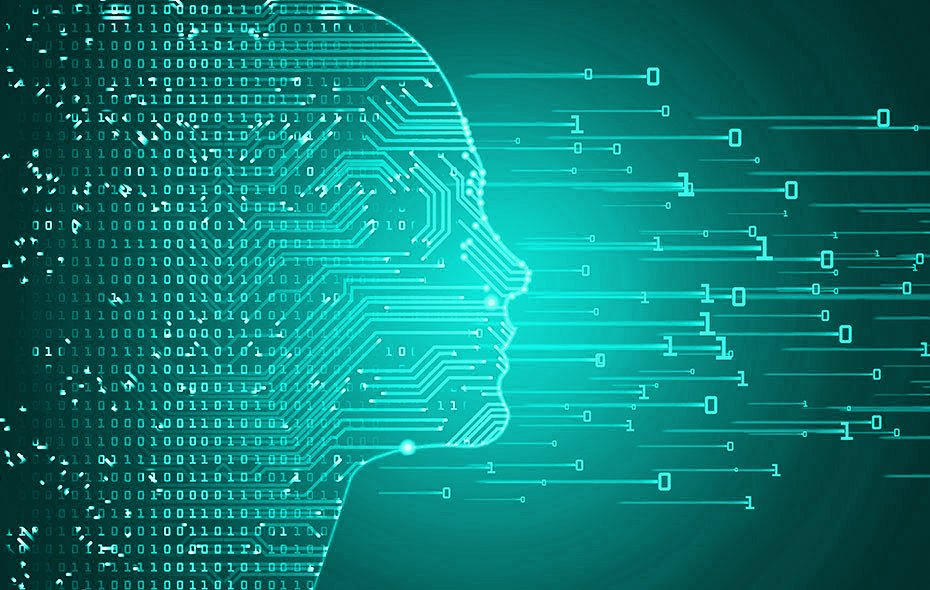
\includegraphics[width=220mm,height=80mm]{Allgemein/LogoDataScienceGruenBlau}};
	
	\vspace{20mm}
	
	
	
	{\hspace{-50mm}%\vspace{-30mm}
		\begin{tikzpicture}
			\draw[Arduino,fill] (0,-1) -- (0,2) -- (80,2) -- (80,-1) -- cycle;
			
			
			\node[black,right] (Name) at (3,3) {\Huge \textsf{Elmar Wings}};
			\node[white,right] (Title) at (3,1) {\Huge \textsf{\TRANS{Künstliche Intelligenz mit dem Arduino Nano 33 BLE Sense}{Artificial Intelligence with an Arduino Nano 33 BLE Sense}}};
			\node[white,right] (Title) at (3,0) {\LARGE \textsf{\TRANS{Echtzeit-Objekterkennung mit der ArduCAM}{Realtime Object Detection with the ArduCAM}}};
			%  \node (logo) at (0,10) {\hspace{-50mm}\vspace{-10mm}\includegraphics[width=220mm,height=80mm]{Allgemein/LogoDataScience.jpg}};
		\end{tikzpicture}
	}
	
	%
	%\begin{minipage}[X]{0.8\textwidth}
	%\begin{tikzpicture}
	%  \draw[black] (0,0) -- (0,10) -- (10,20) -- (10,0) -- cycle;
	%  \node (logo) at (0,10) {\hspace{-50mm}\vspace{-10mm}\includegraphics[width=220mm,height=80mm]{Allgemein/LogoDataScience.jpg}};
	%\end{tikzpicture}
	%\end{minipage}
	%\includegraphics[width=1.4\textwidth]{Allgemein/LogoDataScience.jpg}\hfill
	
	\vfill
	\begin{tabular}{l}
		{$ $Version: 1765 $ $}\\
		\today\\
	\end{tabular}		
	%	\hfill
\includegraphics[width=0.4\textwidth]{Bilder/Technik.jpg} \par\vspace{1cm}
	
	
	
\end{titlepage}

\newpage



\tableofcontents
\newpage

\listoffigures
\newpage

%%%%%%%%%%%%%%%%%%%%%%%%%%%%%%
%
% $Autor: Wings $
% $Datum: 2020-01-29 07:55:27Z $
% $Pfad: komponenten/Bilderkennung/Produktspezifikation/IntelNCS2/Inhalt/Symbollist.tex $
% $Version: 1785 $
%
%
%%%%%%%%%%%%%%%%%%%%%%%%%%%%%%


\chapter*{Verzeichnis der Symbole}
\addcontentsline{toc}{chapter}{Verzeichnis der Symbole}

\markboth{Verzeichnis der Symbole}{Verzeichnis der Symbole}

%\chaptermark{Verzeichnis der Symbole}
%\chaptername


\begin{longtable}{cl}
  API        & Application Programming Interface \\
  COCO       & Common Objects in Context\\
  SDK        & Software Developer Kit \\
  TPU        & Tensor Processor Unit \\
\end{longtable}
\newpage


\InputLanguage{../Inhalt/General/}{Acronymlist}
\newpage

%\Ausblenden
{
	\input{todo}


}


\part{\TRANS{Maschinelles Lernen}{Machine Learning}}

%\Ausblenden
{
	\InputLanguage{../Inhalt/General/}{ki}
	%%%%%%
%
% $Autor: Wings $
% $Datum: 2020-01-18 11:15:45Z $
% $Pfad: WuSt/Skript/Produktspezifikation/powerpoint/ImageProcessing.tex $
% $Version: 4620 $
%
%%%%%%


\section{Grenzen der Künstlichen Intelligenz}

Die Bilderkennung hat in den letzten Jahren riesige Fortschritte gemacht \cite{}. Trotzdem zeigen sich auch Grenzen. In diesem Zusammenhang wird das Bild eines Pandas aus einem Paper von Ian Goodfellow und anderen Forschern gezeigt \cite{Goodfellow:2014}. Ein Algorithmus identifiziert den Panda mit einer Wahrscheinlichkeit von 57{,}7\%. Wird das Bild mit einem zweiten Bild, das der Mensch als Rauschen wahrnimmt, überlagert, so wird ein Gibbon mit einer Wahrscheinlichkeit von 99{,}3 erkannt, obwohl in den Augen eines Menschen sich das Bild nicht geändert hat. Die Situation ist in Abbildung~\ref{Adversarial:Panda} dargestellt.

\begin{figure}
    \includegraphics[page=3,width=0.9\textwidth,viewport=20 600 560 900,clip]{../../MLbib/Adversarial/1412.6572.pdf}
    
    \caption{Überlagerung des Bilds eines Pandas mit Rauschen  \cite{Goodfellow:2014}}\label{Adversarial:Panda}
\end{figure}

Das Beispiel mit dem Panda ist harmlos. Dagegen können die Auswirkungen im Straßenverkehr verheerend sein. Untersuchungen zeigen, dass durch einfache Manipulation von Verkehrsschildern Künstliche Intelligenz falsche Interpretationen durchführen. \cite{Sitawarin:2018} Durch gezielte Veränderungen eines Bilds können wohldefinierte Manipulationen durchgeführt werden. In der Abbildung~\ref{Adversarial:Stop} wird ein Schild, das ein Tempolimit markiert, durch zusätzliche Flecken in ein Stoppschild verwandelt. 



\begin{figure}
  \centering
  \includegraphics[page=2,width=0.4\textwidth,viewport=20 450 180 600,clip]{../../MLbib/Adversarial/1802.06430.pdf}
    
  \caption{Manipulation von Verkehrsschildern  \cite{Sitawarin:2018}}\label{Adversarial:Stop}
\end{figure}

Umgekehrt kann man aus den neuronalen Netzen ein optimales Bild ermittelt, dass ein Ergebnis mit einer Wahrscheinlichkeit nahe bei 100\% liefert. Dabei entstehen auch Bilder, die das menschliche Auge nicht also solches erkennen könnte. Ein klassisches Beispiel ist der Toaster in der Abbildung~\ref{Adversarial:Toaster}.\cite{Brown:2017}


\begin{figure}
    \includegraphics[page=2,width=0.9\textwidth,viewport=20 470 560 900,clip]{../../MLbib/Adversarial/1712.09665.pdf}
    
    \caption{Optimales Bild zur Identifikation eines Toasters  \cite{Sitawarin:2018}}\label{Adversarial:Toaster}
\end{figure}


	
	\InputLanguage{../Inhalt/General/}{kdd} 
	
	\InputLanguage{../Inhalt/General/}{NeuralNetwork} 
	
	\InputLanguage{../Inhalt/General/}{Images}

	%%%%%%%%%%%%
%
% $Autor: Wings $
% $Datum: 2019-03-05 08:03:15Z $
% $Pfad: Automatisierung/Skript/Produktspezifikation/Powerpoint/AMF.tex $
% $Version: 4250 $
% !TeX spellcheck = en_GB/de_DE
% !TeX encoding = utf8
% !TeX root = filename 
% !TeX TXS-program:bibliography = txs:///biber
%
%%%%%%%%%%%%


\chapter{Computer Vision}

\section{Introduction}

Computer vision (CV) is an interdisciplinary scientific field that deals with how computers can gain high-level understanding from digital images or videos. It is the field of artificial intelligence (AI) that enables computers and systems to derive meaningful information from digital images, videos and other visual inputs — and take actions or make recommendations based on that information. \href{https://bit.ly/3iAQkv7}{Computer Vision} There is a lot of research being done in the computer vision field, but it’s not just research. Real-world applications demonstrate how important computer vision is to endeavors in business, entertainment, transportation, healthcare and everyday life. Scientists and engineers have been trying to develop ways for machines to see and understand visual data using Computer vision and Artificial Intelligence. Fig\ref{Computer Vision Chain} shows some of the application using computer vision.


\begin{figure}[h]
	\centering
	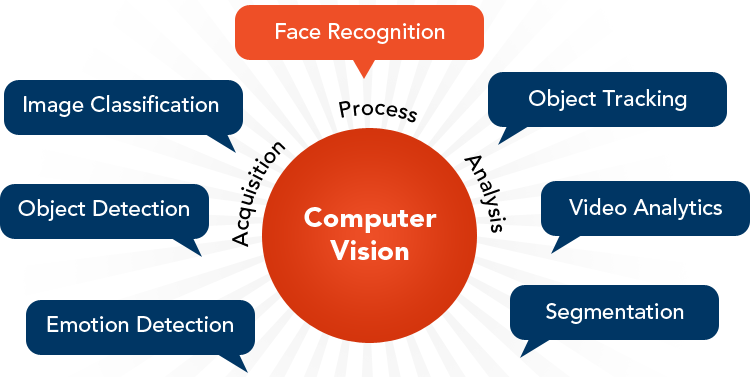
\includegraphics[width=0.7\linewidth]{Nano33BLESense/Computer Vision}
	\caption{Computer Vision Chain}
	\label{Computer Vision Chain}
\end{figure}

Computer Vision enables the computers to see, perceive and understand the world around them. This is achieved through a combination of hardware and software. Computers are trained using lots of images/videos and algorithms/models are built. It uses Convolutional Neural Network (CNN) and is inspired by how the human visual cortex works, processing visual sensory inputs via a hierarchy of layers of neurons.

\section{Use Cases of Computer Vision}

\subsection{Image Classification}

Automate image categorization and organization. This technology is also used for visual search engines.

\subsection{Object Detection}

Automate processes by detecting objects, defects and anomalies in images. Widely used in image retrieval and video surveillance.

\subsection{Video Analytics}

Analyze video content to determine temporal and spatial events like smoke, tamper and motion detection.

\subsection{Image Segmentation}

Image segmentation is the process of partitioning a digital image into multiple segments. Applications include machine vision and video surveillance.

\subsection{Facial Recognition}

Identify a person from a digital image or video. Applications are typically in biometric access control for security systems.

\subsection{Emotion Analysis}

Analyze human faces in images and video to detect the sentiments of the person. Computer vision supports the MediaPipe framework which is also usefull for detecting the Gestures recognition. 


\subsection{Gesture Recognition}

Gesture recognition is a computing process that attempts to recognize and interpret human gestures through the use of mathematical algorithms. \href{https://www.marxentlabs.com/what-is-gesture-recognition-defined/}{Gesture Recognition}It is a type of perceptual computing user interface that allows computers to capture and interpret human gestures as commands. The general definition of gesture recognition is the ability of a computer to understand gestures and execute commands based on those gestures.  

	
	
	\InputLanguage{../Inhalt/General/}{cnn} 
	
	\input{../Inhalt/General/Databases}
	
	\InputLanguage{../Inhalt/General/}{Frameworks}
}


\part{\TRANS{Nano 33 BLE Sense}{Nano 33 BLE Sense}}
	
%%%%%%%%%%%%%%%
%
% $Autor: Wings $
% $Datum: 2020-01-29 07:55:27Z $
% $Pfad: komponenten/Bilderkennung/Produktspezifikation/IntelNCS2/Inhalt/Einleitung.tex $
% $Version: 1785 $
%
%
%%%%%%%%%%%%%%%


%todo citatzions in correct manner
\chapter{Einleitung}


{\tiny Quelle: \url{https://www.arduino.cc/pro/tutorials/portenta-h7}}


\chapter{Indroduction}


Arduino is an open-source electronics platform based on flexible, easy-to-use hardware and software. It provide us on board microcontroller and microprocessor kits for making digital and analogue devices. The microcontroller, oftenly called as tiny computer embed on the arduino board, normally in order to run these microcontroller we need some type of electronics e.g; diodes, resisters, capacitors, and transistors for making the voltage and current balancing. But the arduino team make a user friendly environment for getting rid of these electronics complication to run the hardware on software, just power the board as per the required voltage write the desired programm and upload it in a few seconds, it will bring everything on the board and  make us independent from any worry about the electronics complication. By the technological advancement in semiconductor and electronics  industry, the  control problems are now being solved by using these small size microcontroller instead of mechanical and electrical swithes. All Arduino boards have one thing in common which is a microcontroller, it is basically a really small computer, which help us to make a edge computing application.\cite{Arduino:2021b}

\section{Arduino Nano 33 BLE Sense}


Arduino Nano 33 BLE Sense is one type of arduino family board, which is come up with bluetooth capability for communication and set of sensors. This compact and reliable Nano board is built around the NINA B306 module for BLE and Bluetooth 5.0 communication; Bluetooth 5.0 is the latest version of the Bluetooth wireless communication standard. Use of microcontrollers has become inevitable in almost every field of engineering.  The Arduino Nano 33 BLE Sense module is based on Nordic nRF52480 processor that contains a powerful Cortex M4F and the board has a rich set of sensors that allow the creation of innovative and highly interactive designs. Its reduced power consumption, compared to other same size boards, together with the Nano form factor opens up a wide range of applications. The following figure ~\ref{Arduino Nano} shows a Arduino Nano 33 BLE Sense, shows how compact it is and small in size.

\begin{figure}[ht]
	\centering
	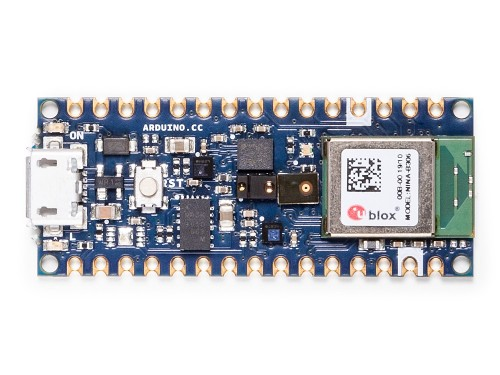
\includegraphics[width=0.45\linewidth]{Arduino/ArduinoNano33BLESense}
	\caption{Arduino Nano 33 BLE Sense} 
	\label{Arduino Nano}
\end{figure}

Due to the Bluetooth low energy (BLE) and set of sensors which are emded on it, this arduino board makes a perfect match for tiny Machine learning and IOT application. Bluetooth is used for communication between Arduino board and external devices. 

\section{On-Board Sensor Description}

Arduino Nano 33 BLE sense come up with the set of embed sensor on the board. The available embed sensors are commonly use for measuring both the analog and digital values around the sorrounding. Arduino Nano 33 BLE sense is very small (45x18)mm in size, which  makes it very usefull for Internet of things (IOT) and Artificial intelligence (AI) application as a embed device where space is the main constrained issue. It is low power consumption board and operate normally on 3.3 V, we can say that this small size low power consumption board can operate on small batteries even for many months. Due to on-board available sensor, the low power consumption and mini architecture we can use this nano board anywhere. The Arduino Nano 33 BLE Sense is a completely new board on a well-known form factor. For getting detail information about each component of Arduino Nano 33 BLE Sense and data sheets of each sensor the following links give us a detail information \cite{ArduinoNano33:2021}. The short description of each sensor are as follow. 

\begin{itemize}
	\item The ADPS-9960 is a digital proximity, ambient light, RGB and gesture sensor. it can measure the proximity distance, light, color and gestures when moving close with the borad.
	\item The LPS22HB is a barometric pressure sensor, it measures the environmental pressure which is usefull for simple weather station monitoring. 
	\item The LSM9DS1 is a 9 axis inertial measurement unit (IMU) use as a Accelerometre, gyroscope, and magnatometre, this 9 axis (IMU) sensor is ideal for wearable devices.
	\item The HTS221 sensor senses the relative humidity, and temperature, to get highly accurate measurements of the environmental conditions.
	\item The MP34DT05 is the digital microphone. it is usefull for capturing, analyzing and detecting the sound in real time.
\end{itemize}

The below figure \ref{Arduino Nano 33 BLE Sense Architecture} show the embed sensors on the board, with powerful processor as compared to other arduino boards the nRF52840 from Nordic Semiconductors, a 32-bit ARM® Cortex™-M4 CPU processor running at 64 MHz are as follow.

\begin{figure}[ht]
	\centering
	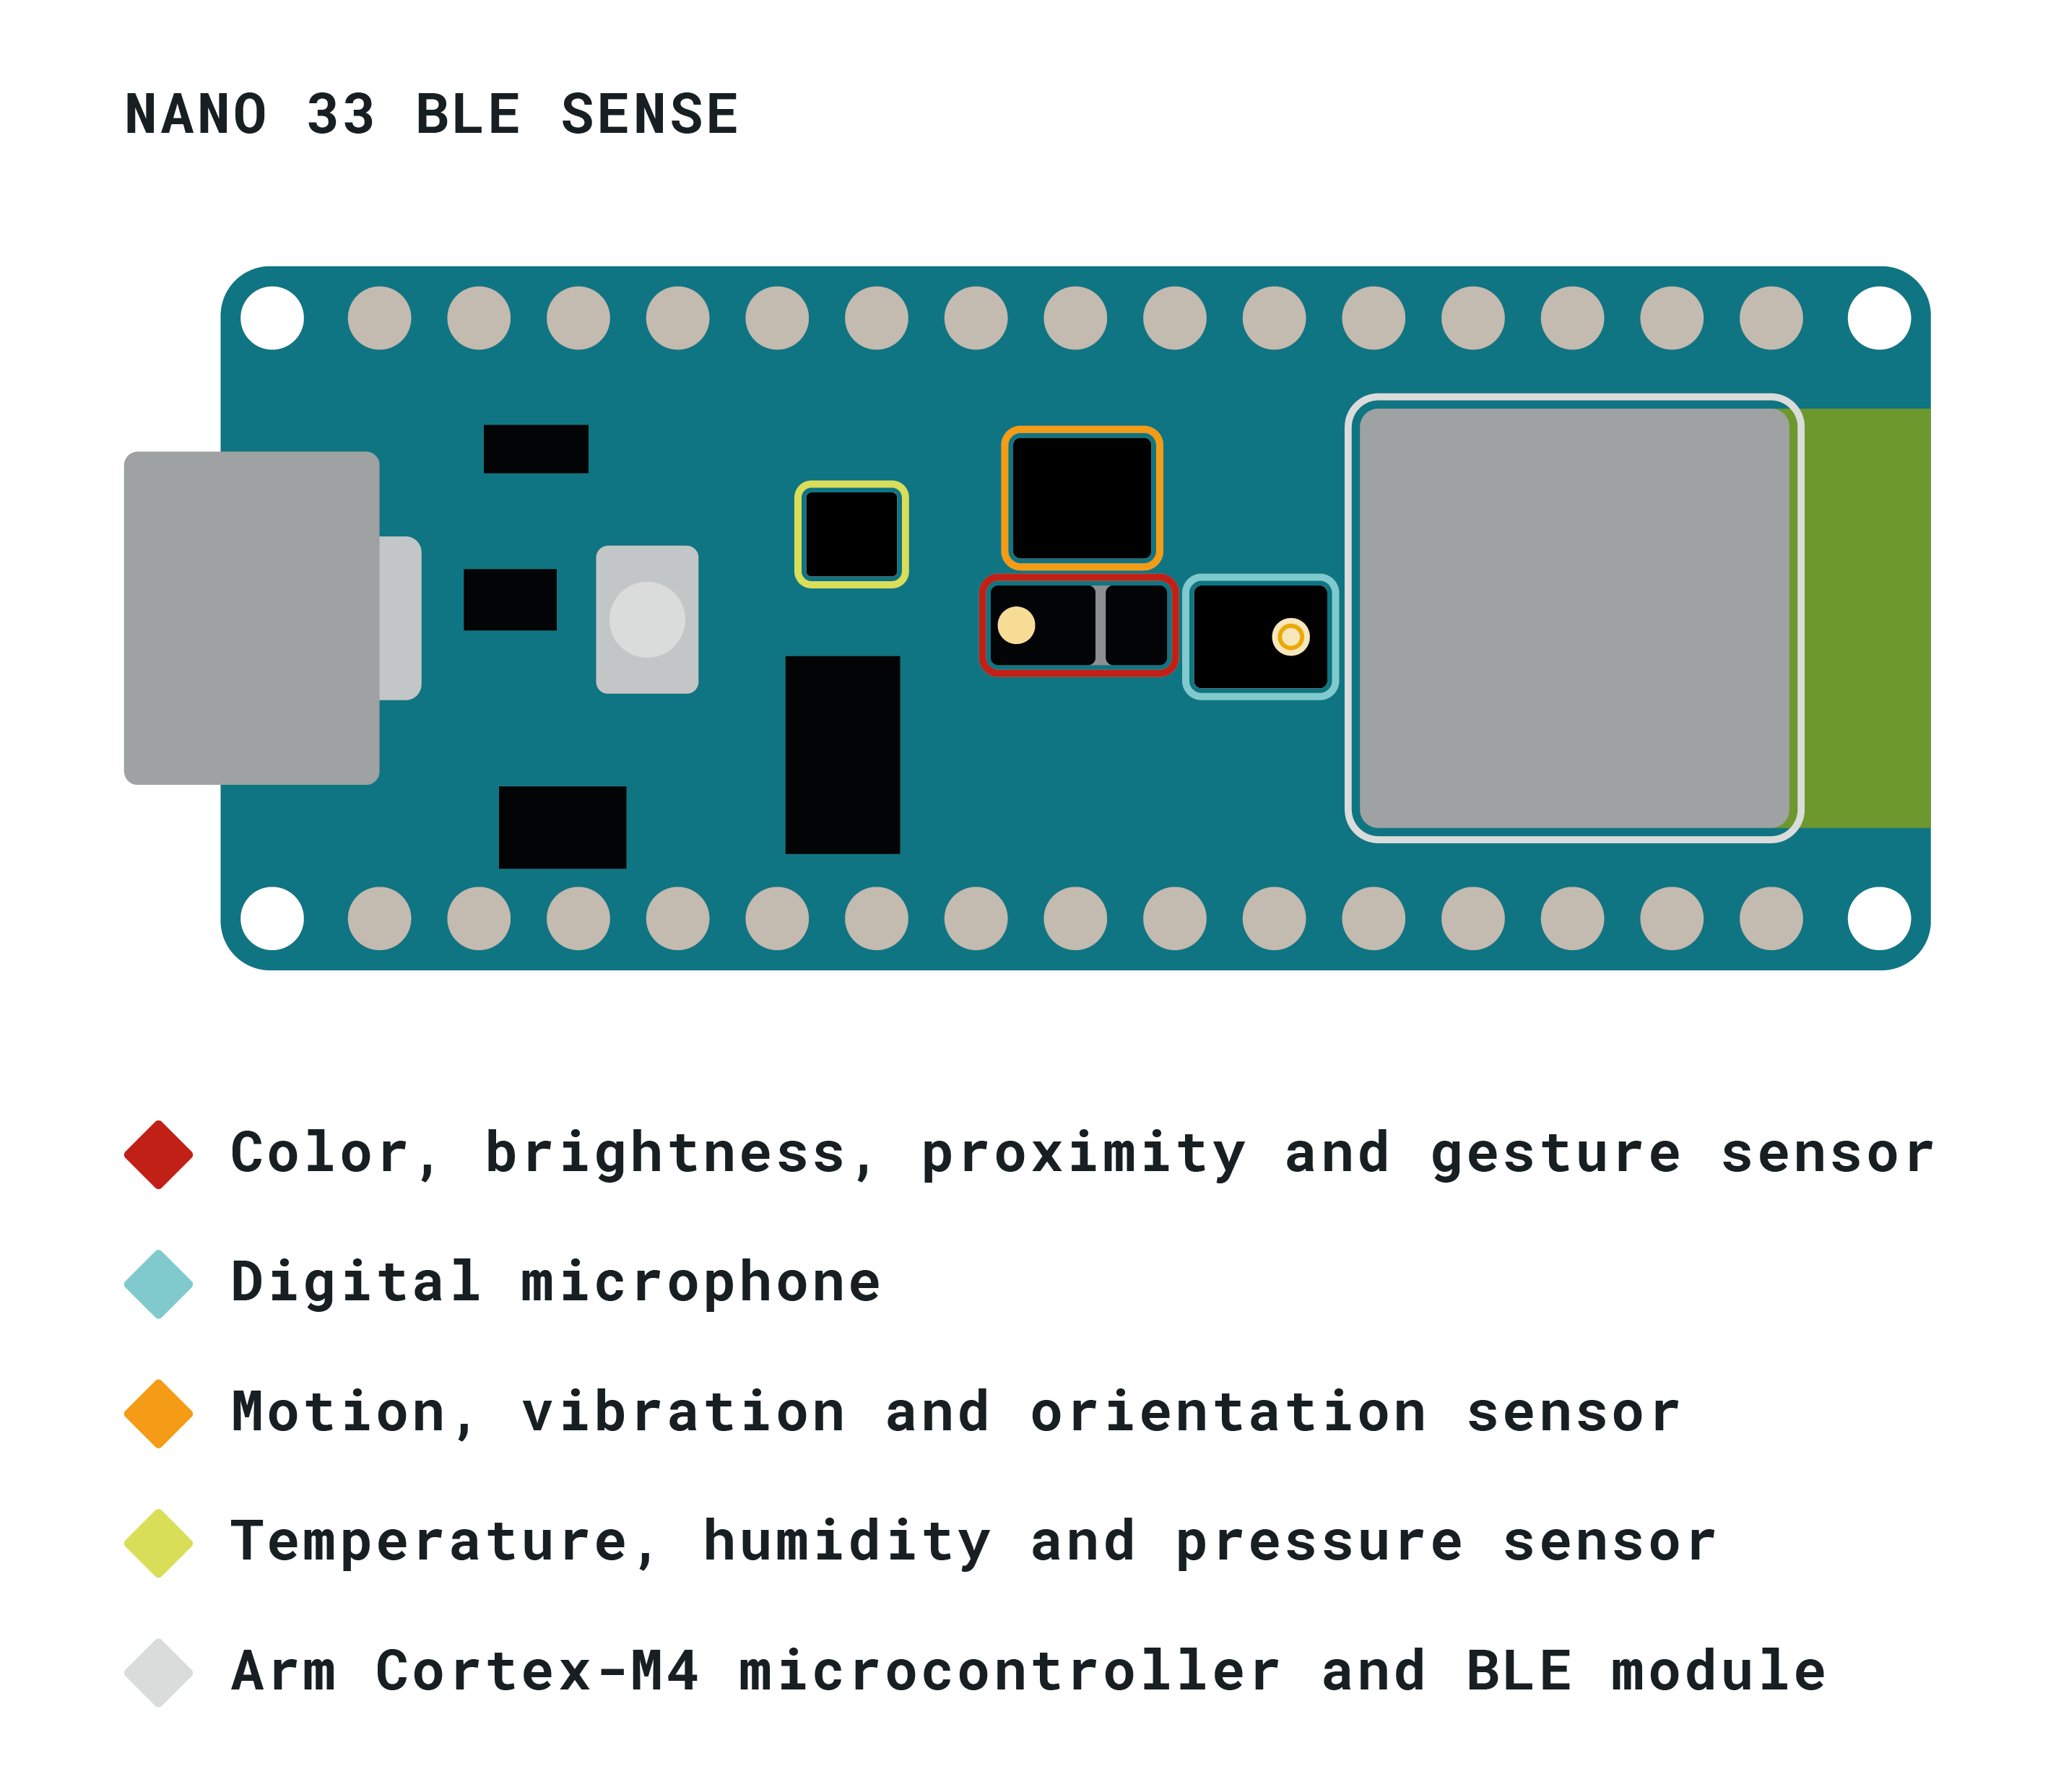
\includegraphics[width=0.5\linewidth]{Nano33BLESense/NANO-33-BLE-Sense_sensor-indentification}
	\caption{Arduino Nano 33 BLE Sense Sensors Placement} 
	\label{Arduino Nano 33 BLE Sense Architecture}
\end{figure}

The Arduino Nano 33 BLE Sense is an evolution of the traditional Arduino Nano, but featuring a lot more powerful processor, the nRF52840 from Nordic Semiconductors, a 32-bit ARM® Cortex™-M4 CPU running at 64 MHz.\cite{ArduinoNano33:2021} This will allow you to make larger programs than with the Arduino Uno (it has 1MB of program memory, 32 times bigger), and with a lot more variables (the RAM is 128 times bigger). The main processor includes other amazing features like Bluetooth® pairing via NFC and ultra low power consumption modes.

\section{Tiny-ML on Arduino Nano 33 BLE Sense}

Machine learning (ML) and Artificial intelligence (AI) are everywhere, its application, use cases and importance make it very usefull for every process. In the same sense, the tiny Arduino nano 33 BLE Sense board give us a way to make Tiny-ML application, where the model are not as big as previuosly made for high and big processing computer. By having a tiny machine learning model we can deploy it on low power devices, one of these is Arduino nano 33 BLE Sense. Due to its small size, the available set of sensors and low power consumption, it is easy to use anywhere by deploying the Machine leaarning algorithm and run the Internet of things (IOT) and Articial intelligence (AI) application for any process.\cite{Dokic:2020}

\section{Usefull Tiny-ML Model for Arduino Nano 33 BLE Sense}

\subsection{Voice Recognition}

Although, being a low power processing device it is not supported the big model and very big data. One of the usefull Tiny-ML model we can make on arduino nano 33 BLE Sense is to detect the different voices from the sorrounding. There is a on-board embed sensor on arduino for detecting voices is MP34DT05 the digital microphone. By using the MP34DT05, we can make a data set for keyword voice recognition model. Initially we train a model on Google colab and then convert it into TensorFlow lite for low power devices.\cite{Waqar:2021} For using the Voice recognition functionality of arduino nano 33 ble board, we need the on-board sensor MP34DT05 (Microphone), which is use for capturing, recognizing and detecting the voice. The supporting library for activating this sensor is PDM which will be discussed in the later chapter.

\subsection{Custom Gesture Recognition}

For capturing the gesture data using the on-board 9-axis Inertial measurement unit (IMU), we can make different types of gestures by rotating and changing the position by holding the arduino board in our hand . By doing this, the 9-axis IMU changes the accelerometre, and gyroscope value of the sensor. The limitation for training this model is to hold the board in our hand all the time. But, for the testing purpose it changes the valuse as per the gesture as shown in the figure below \ref{IMU Sensor Capture Data} for training the Tiny-Ml model.\cite{ArduinoNano33:2021}

\begin{figure}[ht]
	\centering
	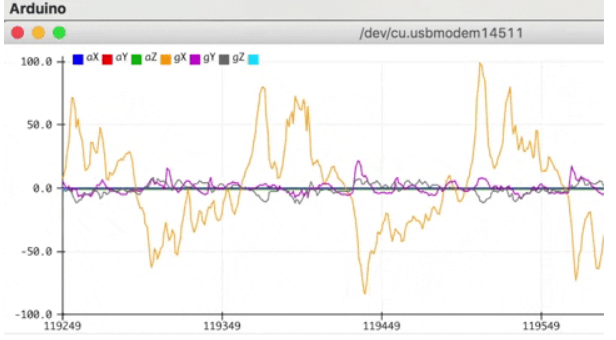
\includegraphics[width=0.5\linewidth]{Nano33BLESense/IMUData}
	\caption{IMU (Inertial Measurement Unit) Gesture Data} 
	\label{IMU Sensor Capture Data}
\end{figure}

The another possibility for detecting gesture is to use the APDS9960 sensor, it can also detect the gesture by moving the hand in front of it. It has also some limitation, it will not detect any gesture above 15 mm distance from the sensor.

\subsection{Color Detection}

The same above mentioned sensor APDS9960 is use for (Red, Green, Blue) RGB color detection too. We can also use the RGB functionality of this sensor and train the Tiny-ML model for detecting the different color product, which make the differentiation among the product on the basis of RGB color.

\subsection{Person Detection} 

One of the advantages of using a small devices such as the Arduino Nano 33 BLE Sense with TinyML is that it could be used as a remote low powered sensor to detect movement or even if there is a person in the area or not. APDS9960 sensor working as a proximity sensor, it can start to detect person at the certain distance. For doing this, we need external camera which can detect the moving person in the sorrounding or not. The supporting camera can be a Arducam Mini 2MP, which will be discuused in the hardware setup chapter later. Some usefull libraries e.g; JPEGDecoder library to decode JPEG-encoded images, the Arducam Library  need to be installed to make the compatibility between Arducam and edge computer (Arduino Nano 33 BLE Sense) by setting the hardware parametre in the library folder. The most necassary setting will be discussed in the later chapters too. \href{https://www.element14.com/community/community/project14/nano-rama/blog/2020/04/29/tinyml-on-arduino-nano-33-ble-sense-person-detection-with-ble}{Person Detection}

\section{General Overview Arduino Board}

Arduino consists of both a physical programmable circuit board (often referred to as a microcontroller) and a piece of software, or Integrated Development Environment (IDE) that runs on our computer, used to write and upload computer code to the physical board. Most of the arduino boards have both analog and digital General purpose input/output (GPIO) pins integrated on the board, depends upon the usage and functionality of the microcontroller embed on arduino board, these multipurpose GPIO makes it more usefull. By the advent of arduino, it make ease and get rid of external programming devices, we dont need to plug in and plug out our microcontrooler for programing the microcontroller. Arduino just need a connection with the computer with the help of USB, and we can upload the programm in a few second. \cite{Arduino:2021b}




\chapter{Hardware}

%%%%%%%%%%%%%%%%%%%%%%%%
%
% $Autor: Wings $
% $Datum: 2019-07-09 09:26:07Z $
% $Pfad: Vorlesungen/WS_19_20/Projekte/KandaNeuralnetwork/latex - Ausarbeitung/Kapitel/Hardware.tex $
% $Version: 4440 $
%
%%%%%%%%%%%%%%%%%%%%%%%%


%todo GitLab\ToDo\TinyML
% TinyML Seite 222

\section{Arduino Nano 33 BLE Sense}



\url{https://www.reichelt.de/de/de/arduino-nano-33-ble-sense-nrf52840-ohne-header-ard-nano-33bles-p261306.html?PROVID=2788&gclid=Cj0KCQjwna2FBhDPARIsACAEc_Uui0sowk2McNvt69o9wzQJtqHWW2n5l_OHng2pSRcmfYqUsiosbdUaAp47EALw_wcB&&r=1}

\subsection{ARD NANO 33BLE S}

Arduino Nano BLE Sense - klein, stromsparend und mit Bluetooth, basierend auf dem  Microcontroller nRF52480.

Dieses kompakte und zuverlässige Nano-Board enthält das Modul NINA B306 für BLE- und Bluetooth 5-Kommunikation. Das Modul basiert auf dem nordischen Prozessor nRF 52840, der einen leistungsstarken Cortex M4F enthält. Es verfügt über einen großen Satz an Sensoren, die die Erstellung innovativer und interaktiver Designs ermöglichen.

Seine Architektur, die vollständig mit Arduino IDE Online und Offline kompatibel ist, verfügt über eine 9-achsige Trägheitsmesseinheit (IMU) mit Temperatur-, Druck-, Feuchtigkeits-, Licht-, Farb- und sogar Gestensensoren sowie über ein Mikrofon, das über die spezialisierten Bibliotheken verwaltet wird. Der im Vergleich zu anderen Boards gleicher Größe geringere Stromverbrauch und der Nano-Formfaktor eröffnen ein breites Anwendungsspektrum.

Dies ermöglicht die Entwicklung von tragbaren Geräten und gestenbasierten Projekten, die mit anderen Geräten aus nächster Nähe kommunizieren müssen.

Der Arduino Nano 33 BLE Sense ist dank des Multiprotokolls BT 5.0 Radio ideal für interaktive Automatisierungsprojekte.

Hinweis: Dieses Board wird ohne integriertem Header geliefert.



\url{https://store.arduino.cc/arduino-nano-33-ble-sense}


\begin{figure}[!h]
  \centering
  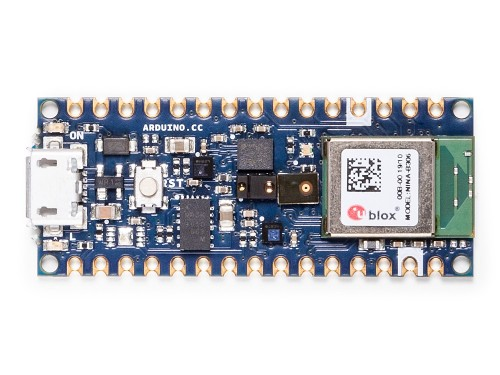
\includegraphics[width=50mm]{Arduino/ArduinoNano33BLESense}
  
  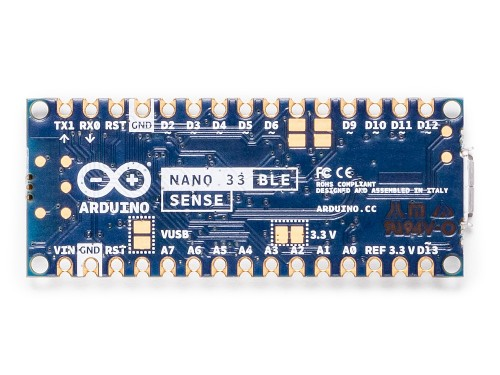
\includegraphics[width=50mm]{Arduino/ArduinoNano33BLESense2}
  
  \caption{Arduino Nano 33 BLE Sense \href{https://store.arduino.cc/arduino-nano-33-ble-sense}{Arduino Store}}
\end{figure}


\section{Tutorial}



\subsection{Was wir bauen}

Wir werden eine eingebettete Anwendung erstellen, die ein Modell zur Klassifizierung von Bildern verwendet, die von einer Kamera aufgenommen wurden. Das Modell wird so trainiert, dass es erkennt, wenn eine Person in der Kameraeingabe vorhanden ist. Das bedeutet, dass unsere Anwendung in der Lage sein wird, die An- oder Abwesenheit einer Person zu erkennen und eine entsprechende Ausgabe zu erzeugen.

Dies ist im Wesentlichen der intelligente Vision-Sensor, den wir etwas früher beschrieben haben. Wenn eine Person erkannt wird, lässt unser Beispielcode eine LED aufleuchten - aber Sie können ihn erweitern, um alle möglichen Projekte zu steuern.

\url{https://github.com/tensorflow/tensorflow/tree/master/tensorflow/lite/micro/examples/person_detection}


\subsection{Bemerkung}

TensorFlow Lite fügt regelmäßig Unterstützung für neue Geräte hinzu. Wenn also das Gerät, das Sie verwenden möchten, hier nicht aufgeführt ist, lohnt es sich, in der \FILE{README.md} des Beispiels nachzusehen. Sie können dort auch nach aktualisierten Deployment-Anweisungen suchen, wenn Sie bei der Ausführung dieser Schritte auf Probleme stoßen.


Anders als bei den vorherigen Kapiteln benötigen Sie für diese Anwendung zusätzliche Hardware. Da keines der beiden Boards eine integrierte Kamera hat, empfehlen wir den Kauf eines Kameramoduls. Diese Informationen finden Sie im Abschnitt über das jeweilige Gerät.

\subsection{Kamera-Module}

Kameramodule sind elektronische Bauteile auf Basis von Bildsensoren, die Bilddaten digital erfassen. Der Bildsensor wird mit einem Objektiv und einer Steuerelektronik kombiniert und das Modul wird in einer Form hergestellt, die einfach an ein Elektronikprojekt angebracht werden kann.

Lassen Sie uns zunächst die Struktur unserer Anwendung durchgehen. Es ist viel einfacher, als Sie vielleicht erwarten.


\subsection{Anwendungsarchitektur}

Inzwischen haben wir festgestellt, dass eingebettete Anwendungen für maschinelles Lernen die folgende Abfolge von Dingen tun:

\begin{itemize}
  \item Erhalten Sie eine Eingabe.
  \item Verarbeiten Sie die Eingabe vor, um Merkmale zu extrahieren, die für die Eingabe in ein Modell geeignet sind.
  \item Ausführen der Inferenz auf die verarbeitete Eingabe.
  \item Die Ausgabe des Modells nachverarbeiten, um sie sinnvoll zu nutzen.
  \item Verwenden Sie die resultierenden Informationen, um etwas zu bewirken.
\end{itemize}

In Kapitel 7 haben wir gesehen, wie dies auf die Wake-Word-Erkennung angewendet wird, die Audio als Eingabe verwendet. Dieses Mal werden wir als Eingabe Bilddaten verwenden. Das hört sich vielleicht komplizierter an, ist aber in Wirklichkeit viel einfacher zu handhaben als Audio.

Bilddaten werden üblicherweise als ein Array von Pixelwerten dargestellt. Wir werden unsere Bilddaten von eingebetteten Kameramodulen beziehen, die alle Daten in diesem Format bereitstellen. Unser Modell erwartet auch, dass seine Eingabe ein Array von Pixelwerten ist. Aus diesem Grund müssen wir nicht viel Vorarbeit leisten, bevor wir die Daten in unser Modell einspeisen.

Angesichts der Tatsache, dass wir nicht viel Vorverarbeitung machen müssen, wird unsere Anwendung ziemlich einfach sein. Sie nimmt einen Schnappschuss der Daten von einer Kamera auf, speist ihn in ein Modell ein und bestimmt, welche Ausgabeklasse erkannt wurde. Anschließend zeigt sie das Ergebnis auf einfache Weise an.

Bevor wir weitermachen, wollen wir ein wenig mehr über das Modell erfahren, das wir verwenden werden.

\subsection{Einführung in unser Modell}

In Kapitel 7 haben wir gelernt, dass faltungsneuronale Netze neuronale Netze sind, die für die Arbeit mit mehrdimensionalen Tensoren ausgelegt sind, bei denen die Informationen in den Beziehungen zwischen Gruppen benachbarter Werte enthalten sind. Sie sind besonders gut für die Arbeit mit Bilddaten geeignet.

Unser Personenerkennungsmodell ist ein neuronales Faltungsnetzwerk, das auf dem Visual Wake Words-Datensatz trainiert wurde. Dieser Datensatz besteht aus 115.000 Bildern, von denen jedes mit der Angabe versehen ist, ob es eine Person enthält oder nicht.

Das Modell ist 250 KB groß und damit deutlich größer als unser Sprachmodell. Diese zusätzliche Größe belegt nicht nur mehr Speicher, sondern bedeutet auch, dass es viel länger dauert, eine einzelne Inferenz auszuführen.

Das Modell akzeptiert 96 × 96-Pixel-Graustufenbilder als Eingabe. Jedes Bild wird als 3D-Tensor mit der Form (96, 96, 1) bereitgestellt, wobei die letzte Dimension einen 8-Bit-Wert enthält, der ein einzelnes Pixel repräsentiert. Der Wert gibt den Farbton des Pixels an, der von 0 (vollständig schwarz) bis 255 (vollständig weiß) reicht.

Unsere Kameramodule können Bilder in verschiedenen Auflösungen zurückgeben, daher müssen wir sicherstellen, dass sie auf 96 × 96 Pixel verkleinert werden. Außerdem müssen wir vollfarbige Bilder in Graustufen umwandeln, damit sie mit dem Modell funktionieren.

\url{https://arxiv.org/abs/1906.05721}


Sie denken vielleicht, dass 96 × 96 Pixel eine winzige Auflösung ist, aber sie ist mehr als ausreichend, um eine Person in jedem Bild zu erkennen. Modelle, die mit Bildern arbeiten, akzeptieren oft erstaunlich kleine Auflösungen. Eine Erhöhung der Eingabegröße eines Modells führt zu abnehmenden Erträgen, und die Komplexität des Netzwerks steigt stark an, wenn die Größe der Eingabe skaliert. Aus diesem Grund arbeiten selbst moderne Bildklassifizierungsmodelle in der Regel mit einer maximalen Auflösung von 320 × 320 Pixeln.

Das Modell gibt zwei Wahrscheinlichkeiten aus: eine, die die Wahrscheinlichkeit angibt, dass eine Person in der Eingabe vorhanden war, und eine andere, die die Wahrscheinlichkeit angibt, dass niemand dort war. Die Wahrscheinlichkeiten reichen von 0 bis 255.

Unser Personenerkennungsmodell verwendet die MobileNet-Architektur, eine bekannte und erprobte Architektur, die für die Bildklassifizierung auf Geräten wie Mobiltelefonen entwickelt wurde. In Kapitel 10 werden Sie erfahren, wie dieses Modell an Mikrocontroller angepasst wurde und wie Sie Ihr eigenes Modell trainieren können. Lassen Sie uns nun weiter erkunden, wie unsere Anwendung funktioniert.


\subsection{Alle beweglichen Teile}


Figure~\ref{tflite:Ablauf} shows the structure of our person detection application.

\begin{figure}
  \centering
  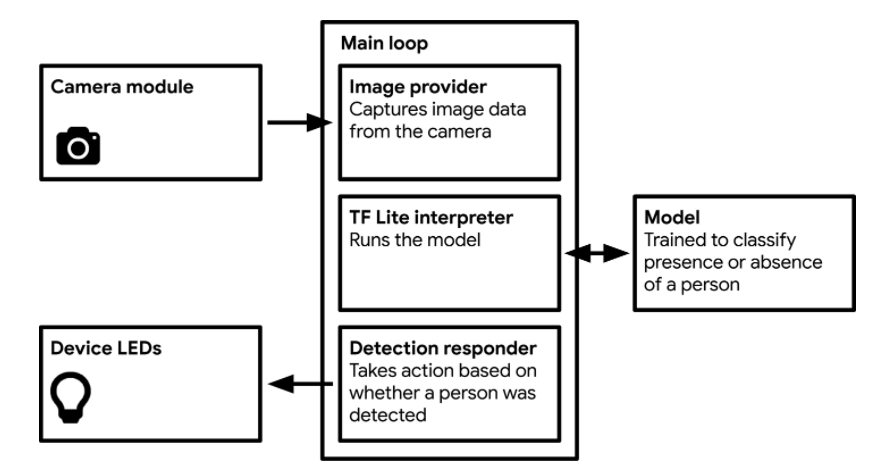
\includegraphics[width=0.9\textwidth]{Arduino/tfLiteAblauf}
  \caption{Diagram of the components of our person detection application}\label{tflite:Ablauf}
\end{figure}

Wie wir bereits erwähnt haben, ist dies viel einfacher als die Wake-Word-Anwendung, da wir die Bilddaten direkt in das Modell übergeben können - es ist keine Vorverarbeitung erforderlich.

Ein weiterer Aspekt, der die Dinge einfach hält, ist, dass wir die Ausgabe des Modells nicht mitteln. Unser Wake-Word-Modell wurde mehrmals pro Sekunde ausgeführt, so dass wir seine Ausgabe mitteln mussten, um ein stabiles Ergebnis zu erhalten. Unser Personenerkennungsmodell ist viel größer und braucht viel länger, um die Inferenz auszuführen. Das bedeutet, dass es keine Notwendigkeit gibt, seine Ausgabe zu mitteln.

Der Code besteht aus fünf Hauptteilen:

\textbf{Main loop}

Wie die anderen Beispiele läuft auch unsere Anwendung in einer Endlosschleife. Da unser Modell jedoch viel größer und komplexer ist, dauert es länger, bis die Inferenz ausgeführt wird. Je nach Gerät können wir eine Inferenz alle paar Sekunden erwarten, anstatt mehrere Inferenzen pro Sekunde.

\textbf{Image provider}

Diese Komponente erfasst Bilddaten von der Kamera und schreibt sie in den Eingangstensor. Die Methoden zur Erfassung von Bildern variieren von Gerät zu Gerät, daher kann diese Komponente überschrieben und angepasst werden.

\textbf{TensorFlow Lite interpreter}

Der Interpreter führt das TensorFlow Lite Modell aus und transformiert das Eingabebild in einen Satz von Wahrscheinlichkeiten.

\textbf{Modell}

Das Modell wird als Datenarray eingebunden und vom Interpreter ausgeführt. Mit 250 KB ist dieses Modell unangemessen groß, um es an das TensorFlow GitHub Repository zu übergeben. Aus diesem Grund wird es vom Makefile heruntergeladen, wenn das Projekt gebaut wird. Wenn Sie einen Blick darauf werfen wollen, können Sie es selbst unter \FILE{tf\_lite\_micro\_person\_data\_grayscale.zip} herunterladen.

\textbf{Detection responder}


Der Erkennungsresponder nimmt die vom Modell ausgegebenen Wahrscheinlichkeiten und verwendet die Ausgabefähigkeiten des Geräts, um sie anzuzeigen. Wir können ihn für verschiedene Gerätetypen überschreiben. In unserem Beispielcode leuchtet eine LED auf, aber Sie können ihn so erweitern, dass er so ziemlich alles tun kann.

Um ein Gefühl dafür zu bekommen, wie diese Teile zusammenpassen, werfen wir einen Blick auf ihre Tests.

\textbf{Durch die Tests gehen}

Diese Anwendung ist schön einfach, da es nur ein paar Tests zu durchlaufen gibt. Sie können sie alle im GitHub-Repository finden:

\FILE{person\_detection\_test.cc}

Zeigt, wie eine Inferenz auf ein Array, das ein einzelnes Bild repräsentiert, ausgeführt werden kann

\FILE{image\_provider\_test.cc}


Zeigt, wie Sie den Bildanbieter verwenden, um ein Bild aufzunehmen

\FILE{detection\_responder\_test.cc}

Zeigt, wie der Erkennungsresponder verwendet wird, um die Ergebnisse der Erkennung auszugeben.

Beginnen wir mit der Untersuchung von \FILE{person\_detection\_test.cc}, um zu sehen, wie die Inferenz auf Bilddaten ausgeführt wird. Da dies das dritte Beispiel ist, das wir durchlaufen haben, sollte Ihnen dieser Code ziemlich vertraut vorkommen. Sie sind auf dem besten Weg, ein eingebetteter ML-Entwickler zu werden!

\textbf{Der Grundablauf}

Beginnen wir mit der Datei \FILE{Person\_detection\_test.cc}. Wir beginnen damit, dass wir die Ops hineinziehen, die unser Modell benötigen wird:

\begin{code}
    

%\lstinputlisting[firstline=1,lastline=136,firstnumber=10,language=c++]{../Code/Nano33BLESense/person_detection/person_detection_test.cc}    

  \begin{lstlisting}
namespace tflite {
    namespace ops {
        namespace micro {
            TfLiteRegistration* Register_DEPTHWISE_CONV_2D();
            TfLiteRegistration* Register_CONV_2D();
            TfLiteRegistration* Register_AVERAGE_POOL_2D();
        }  // namespace micro
    }  // namespace ops
}  // namespace tflite
  \end{lstlisting}
\end{code}


Als nächstes definieren wir eine Tensor-Arena, die für das Modell angemessen groß ist. Wie üblich wurde diese Zahl durch Versuch und Irrtum ermittelt:


\begin{code}
    \begin{lstlisting}
const int tensor_arena_size = 70 * 1024;
uint8_t tensor_arena[tensor_arena_size];
  \end{lstlisting}
\end{code}

Anschließend führen wir die typischen Einrichtungsarbeiten durch, um den Interpreter einsatzbereit zu machen, wozu auch die Registrierung der erforderlichen Ops mit dem \PYTHON{MicroMutableOpResolver} gehört:

\begin{code}
    \begin{lstlisting}
// Set up logging.
tflite::MicroErrorReporter micro_error_reporter;
tflite::ErrorReporter* error_reporter = &micro_error_reporter;

// Map the model into a usable data structure. This doesn't involve any
// copying or parsing, it's a very lightweight operation.
const tflite::Model* model = ::tflite::GetModel(g_person_detect_model_data);
if (model->version() != TFLITE_SCHEMA_VERSION) {
    error_reporter->Report(
    "Model provided is schema version %d not equal "
    "to supported version %d.\n",
    model->version(), TFLITE_SCHEMA_VERSION);
}

// Pull in only the operation implementations we need.
tflite::MicroMutableOpResolver micro_mutable_op_resolver;
micro_mutable_op_resolver.AddBuiltin(
tflite::BuiltinOperator_DEPTHWISE_CONV_2D,
tflite::ops::micro::Register_DEPTHWISE_CONV_2D());
micro_mutable_op_resolver.AddBuiltin(tflite::BuiltinOperator_CONV_2D,
tflite::ops::micro::Register_CONV_2D());
micro_mutable_op_resolver.AddBuiltin(
tflite::BuiltinOperator_AVERAGE_POOL_2D,
tflite::ops::micro::Register_AVERAGE_POOL_2D());

// Build an interpreter to run the model with.
tflite::MicroInterpreter interpreter(model, micro_mutable_op_resolver,
tensor_arena, tensor_arena_size,
error_reporter);
interpreter.AllocateTensors();
  \end{lstlisting}
\end{code}

Unser nächster Schritt ist die Überprüfung des Eingabetensors. Wir prüfen, ob er die erwartete Anzahl von Dimensionen hat und ob seine Dimensionen angemessen dimensioniert sind:

\begin{code}
    \begin{lstlisting}
// Get information about the memory area to use for the model's input.
TfLiteTensor* input = interpreter.input(0);

// Make sure the input has the properties we expect.
TF_LITE_MICRO_EXPECT_NE(nullptr, input);
TF_LITE_MICRO_EXPECT_EQ(4, input->dims->size);
TF_LITE_MICRO_EXPECT_EQ(1, input->dims->data[0]);
TF_LITE_MICRO_EXPECT_EQ(kNumRows, input->dims->data[1]);
TF_LITE_MICRO_EXPECT_EQ(kNumCols, input->dims->data[2]);
TF_LITE_MICRO_EXPECT_EQ(kNumChannels, input->dims->data[3]);
TF_LITE_MICRO_EXPECT_EQ(kTfLiteUInt8, input->type);
  \end{lstlisting}
\end{code}

Daraus können wir erkennen, dass die Eingabe technisch gesehen ein 5D-Tensor ist. Die erste Dimension ist nur ein Wrapper, der ein einzelnes Element enthält. Die folgenden zwei Dimensionen stellen die Zeilen und Spalten der Pixel des Bildes dar. Die letzte Dimension enthält die Anzahl der Farbkanäle, die zur Darstellung jedes Pixels verwendet werden.

Die Konstanten, die die erwarteten Dimensionen angeben, \PYTHON{kNumRows}, \PYTHON{kNumCols} und \PYTHON{kNumChannels}, sind in \FILE{model\_settings.h} definiert. Sie sehen folgendermaßen aus:

\begin{code}
    \begin{lstlisting}
constexpr int kNumCols = 96;
constexpr int kNumRows = 96;
constexpr int kNumChannels = 1;
  \end{lstlisting}
\end{code}

Wie Sie sehen können, wird erwartet, dass das Modell eine Bitmap mit $96 \times 96$ Pixeln akzeptiert. Das Bild wird in Graustufen dargestellt, mit einem Farbkanal für jedes Pixel.

Als nächstes im Code kopieren wir ein Testbild in den Eingangstensor mit einer einfachen for-Schleife:

\begin{code}
    \begin{lstlisting}
// Copy an image with a person into the memory area used for the input.
const uint8_t* person_data = g_person_data;
for (int i = 0; i < input->bytes; ++i) {
    input->data.uint8[i] = person_data[i];
}
  \end{lstlisting}
\end{code}

Die Variable, die die Bilddaten speichert, \PYTHON{g\_person\_data}, wird in der Datei \FILE{person\_image\_data.h} definiert. Um zu vermeiden, dass dem Repository weitere große Dateien hinzugefügt werden, werden die Daten selbst zusammen mit dem Modell heruntergeladen, als Teil von \FILE{tf\_lite\_micro\_person\_data\_grayscale.zip}, wenn die Tests zum ersten Mal ausgeführt werden.

Nachdem wir den Eingabetensor aufgefüllt haben, führen wir die Inferenz durch. Es ist so einfach wie immer:

\begin{code}
    \begin{lstlisting}
// Run the model on this input and make sure it succeeds.
TfLiteStatus invoke_status = interpreter.Invoke();
if (invoke_status != kTfLiteOk) {
    error_reporter->Report("Invoke failed\n");
}
TF_LITE_MICRO_EXPECT_EQ(kTfLiteOk, invoke_status);
  \end{lstlisting}
\end{code}

Wir überprüfen nun den Ausgangstensor, um sicherzustellen, dass er die erwartete Größe und Form hat:

\begin{code}
    \begin{lstlisting}
TfLiteTensor* output = interpreter.output(0);
TF_LITE_MICRO_EXPECT_EQ(4, output->dims->size);
TF_LITE_MICRO_EXPECT_EQ(1, output->dims->data[0]);
TF_LITE_MICRO_EXPECT_EQ(1, output->dims->data[1]);
TF_LITE_MICRO_EXPECT_EQ(1, output->dims->data[2]);
TF_LITE_MICRO_EXPECT_EQ(kCategoryCount, output->dims->data[3]);
TF_LITE_MICRO_EXPECT_EQ(kTfLiteUInt8, output->type);
  \end{lstlisting}
\end{code}

Die Ausgabe des Modells hat vier Dimensionen. Die ersten drei sind nur Umhüllungen für die vierte, die ein Element für jede Kategorie enthält, für die das Modell trainiert wurde.

Die Gesamtzahl der Kategorien ist als Konstante kCategoryCount verfügbar, die sich zusammen mit einigen anderen hilfreichen Werten in \FILE{model\_settings.h} befindet:

\begin{code}
    \begin{lstlisting}
constexpr int kCategoryCount = 3;
constexpr int kPersonIndex = 1;
constexpr int kNotAPersonIndex = 2;
extern const char* kCategoryLabels[kCategoryCount];
  \end{lstlisting}
\end{code}

Wie \PYTHON{kCategoryCount} zeigt, gibt es drei Kategorien in der Ausgabe. Die erste ist zufällig eine unbenutzte Kategorie, die wir ignorieren können. Die Kategorie "Person" kommt an zweiter Stelle, wie wir an ihrem Index erkennen können, der in der Konstante \PYTHON{kPersonIndex} gespeichert ist. An dritter Stelle steht die Kategorie "keine Person", deren Index durch \PYTHON{kNotAPersonIndex} angezeigt wird.

Es gibt auch ein Array von Kategoriebezeichnungen, kCategoryLabels, das in \FILE{model\_settings.cc} implementiert ist:

\begin{code}
    \begin{lstlisting}
const char* kCategoryLabels[kCategoryCount] = {
    "unused",
    "person",
    "notperson",
};
  \end{lstlisting}
\end{code}



\subsection{Extra Dimensions}

Wie \PYTHON{kCategoryCount} zeigt, gibt es drei Kategorien in der Ausgabe. Die erste ist zufällig eine unbenutzte Kategorie, die wir ignorieren können. Die Kategorie "Person" kommt an zweiter Stelle, wie wir an ihrem Index erkennen können, der in der Konstante kPersonIndex gespeichert ist. An dritter Stelle steht die Kategorie "keine Person", deren Index durch kNotAPersonIndex angezeigt wird.

Es gibt auch ein Array von Kategoriebezeichnungen, \PYTHON{kCategoryLabels}, das in \FILE{model\_settings.cc} implementiert ist:
Wie \PYTHON{kCategoryCount} zeigt, gibt es drei Kategorien in der Ausgabe. Die erste ist zufällig eine unbenutzte Kategorie, die wir ignorieren können. Die Kategorie "Person" kommt an zweiter Stelle, wie wir an ihrem Index erkennen können, der in der Konstante \PYTHON{kPersonIndex} gespeichert ist. An dritter Stelle steht die Kategorie "keine Person", deren Index durch \PYTHON{kNotAPersonIndex} angezeigt wird.

Es gibt auch ein Array von Kategoriebezeichnungen, \PYTHON{kCategoryLabels}, das in \FILE{model\_settings.cc} implementiert ist:

\begin{code}
    \begin{lstlisting}
uint8_t person_score = output->data.uint8[kPersonIndex];
uint8_t no_person_score = output->data.uint8[kNotAPersonIndex];
error_reporter->Report(
"person data.  person score: %d, no person score: %d\n", person_score,
no_person_score);
TF_LITE_MICRO_EXPECT_GT(person_score, no_person_score);
  \end{lstlisting}
\end{code}

Da der einzige Dateninhalt des Ausgabetensors die drei \PYTHON{uint8}-Werte sind, die die Klassenwerte darstellen, wobei der erste unbenutzt ist, können wir direkt auf die Werte zugreifen, indem wir \PYTHON{output->data.uint8[kPersonIndex]} und \PYTHON{output->data.uint8[kNotAPersonIndex]} verwenden. Als uint8-Typen haben sie einen Minimalwert von 0 und einen Maximalwert von 255.





\subsection{NOTE}

Wenn die Werte für "Person" und "keine Person" ähnlich sind, kann dies bedeuten, dass das Modell nicht sehr sicher in seiner Vorhersage ist. In diesem Fall können Sie das Ergebnis als nicht schlüssig betrachten.

Als nächstes testen wir auf ein Bild ohne Person, das von \PYTHON{g\_no\_person\_data} gehalten wird:


\begin{code}
    \begin{lstlisting}
const uint8_t* no_person_data = g_no_person_data;
for (int i = 0; i < input->bytes; ++i) {
    input->data.uint8[i] = no_person_data[i];
}
  \end{lstlisting}
\end{code}


Nachdem die Inferenz gelaufen ist, behaupten wir dann, dass der Wert "keine Person" höher ist:

\begin{code}
    \begin{lstlisting}
person_score = output->data.uint8[kPersonIndex];
no_person_score = output->data.uint8[kNotAPersonIndex];
error_reporter->Report(
"no person data.  person score: %d, no person score: %d\n", person_score,
no_person_score);
TF_LITE_MICRO_EXPECT_GT(no_person_score, person_score);
  \end{lstlisting}
\end{code}

Wie Sie sehen können, geht hier nichts Ausgefallenes vor sich. Wir geben zwar Bilder anstelle von Skalaren oder Spektrogrammen ein, aber der Prozess der Inferenz ist ähnlich zu dem, was wir zuvor gesehen haben.

Das Ausführen des Tests ist ähnlich einfach. Geben Sie einfach den folgenden Befehl aus dem Stammverzeichnis des TensorFlow-Repositorys ein:

\begin{code}
    \begin{lstlisting}
make -f tensorflow/lite/micro/tools/make/Makefile \
test_person_detection_test
  \end{lstlisting}
\end{code}

Wenn der Test das erste Mal ausgeführt wird, werden das Modell und die Bilddaten heruntergeladen. Wenn Sie einen Blick auf die heruntergeladenen Dateien werfen möchten, finden Sie diese in \FILE{tensorflow/lite/micro/tools/make/downloads/person\_model\_grayscale}. Siehe \url{../Code/Nano33BLESense/person_detection_int8}. Achtung ist eine C-Datei.

Als Nächstes schauen wir uns die Schnittstelle für den Bildanbieter an.



\subsection{The Image Provider}

Der Image-Provider ist dafür verantwortlich, Daten von der Kamera abzugreifen und sie in einem Format zurückzugeben, das für das Schreiben in den Eingabetensor des Modells geeignet ist. Die Datei \FILE{image\_provider.h} definiert seine Schnittstelle:

\begin{code}
    \begin{lstlisting}
TfLiteStatus GetImage(tflite::ErrorReporter* error_reporter, int image_width,
int image_height, int channels, uint8_t* image_data);
  \end{lstlisting}
\end{code}

Da die eigentliche Implementierung plattformspezifisch ist, gibt es eine Referenzimplementierung in \FILE{person\_detection/image\_provider.cc}, die Dummy-Daten zurückgibt.

Der Test in \FILE{image\_provider\_test.cc} ruft diese Referenzimplementierung auf, um zu zeigen, wie sie verwendet wird. Als erstes müssen wir ein Array erstellen, das die Bilddaten enthält. Dies geschieht in der folgenden Zeile:

\begin{code}
    \begin{lstlisting}
uint8_t image_data[kMaxImageSize];
  \end{lstlisting}
\end{code}

Die Konstante \PYTHON{kMaxImageSize} stammt aus unserem alten Freund, \FILE{model\_settings.h}.

Nachdem wir dieses Array eingerichtet haben, können wir die Funktion \PYTHON{GetImage()} aufrufen, um ein Bild von der Kamera zu erfassen:

\begin{code}
    \begin{lstlisting}
TfLiteStatus get_status =
GetImage(error_reporter, kNumCols, kNumRows, kNumChannels, image_data);
TF_LITE_MICRO_EXPECT_EQ(kTfLiteOk, get_status);
TF_LITE_MICRO_EXPECT_NE(image_data, nullptr);
  \end{lstlisting}
\end{code}

Wir rufen sie mit einer ErrorReporter-Instanz auf, mit der Anzahl der gewünschten Spalten, Zeilen und Kanäle und mit einem Zeiger auf unser Array \PYTHON{image\_data}. Die Funktion wird die Bilddaten in dieses Array schreiben. Wir können den Rückgabewert der Funktion überprüfen, um festzustellen, ob der Erfassungsprozess erfolgreich war; er wird auf \PYTHON{kTfLiteError} gesetzt, wenn es ein Problem gibt, oder andernfalls auf \PYTHON{kTfLiteOk}.

Schließlich geht der Test durch die zurückgegebenen Daten, um zu zeigen, dass alle Speicherplätze lesbar sind. Auch wenn das Bild technisch gesehen Zeilen, Spalten und Kanäle hat, werden die Daten in der Praxis in ein 1D-Array gepresst:

\begin{code}
    \begin{lstlisting}
uint32_t total = 0;
for (int i = 0; i < kMaxImageSize; ++i) {
    total += image_data[i];
}
  \end{lstlisting}
\end{code}

Um diesen Test auszuführen, verwenden Sie den folgenden Befehl:

\begin{code}
    \begin{lstlisting}
make -f tensorflow/lite/micro/tools/make/Makefile \
test_image_provider_test
  \end{lstlisting}
\end{code}

Wir werden die gerätespezifischen Implementierungen von \FILE{image\_provider.cc} später im Kapitel untersuchen; für den Moment wollen wir uns die Schnittstelle des Erkennungsresponders ansehen.

\subsection{The Detection Responder}

Unser letzter Test zeigt, wie der Erkennungsresponder verwendet wird. Dies ist der Code, der für die Übermittlung der Ergebnisse der Inferenz verantwortlich ist. Seine Schnittstelle ist in \FILE{detection\_responder.h} definiert, und der Test befindet sich in \FILE{detection\_responder\_test.cc}.

Die Schnittstelle ist ziemlich einfach:

\begin{code}
    \begin{lstlisting}
void RespondToDetection(tflite::ErrorReporter* error_reporter,
uint8_t person_score, uint8_t no_person_score);
  \end{lstlisting}
\end{code}

Wir rufen es einfach mit den Werten für die beiden Kategorien "Person" und "keine Person" auf, und es entscheidet, was von da an zu tun ist.

Die Referenzimplementierung in \FILE{detection\_responder.cc} protokolliert nur diese Werte. Der Test in \FILE{detection\_responder\_test.cc} ruft die Funktion ein paar Mal auf:

\begin{code}
    \begin{lstlisting}
RespondToDetection(error_reporter, 100, 200);
RespondToDetection(error_reporter, 200, 100);
  \end{lstlisting}
\end{code}

Um den Test auszuführen und die Ausgabe zu sehen, verwenden Sie den folgenden Befehl:

\begin{code}
    \begin{lstlisting}
make -f tensorflow/lite/micro/tools/make/Makefile \
test_detection_responder_test
  \end{lstlisting}
\end{code}

Wir haben alle Tests und die Schnittstellen, die sie ausüben, erkundet. Lassen Sie uns nun das Programm selbst durchgehen.

\subsection{Detecting People}

Die Kernfunktionen der Anwendung befinden sich in DATEI{main\_functions.cc}. Sie sind kurz und bündig, und wir haben viel von ihrer Logik in den Tests gesehen.

Zuerst holen wir uns alle Funktionen, die unser Modell benötigt:

\begin{code}
    \begin{lstlisting}
namespace tflite {
    namespace ops {
        namespace micro {
            TfLiteRegistration* Register_DEPTHWISE_CONV_2D();
            TfLiteRegistration* Register_CONV_2D();
            TfLiteRegistration* Register_AVERAGE_POOL_2D();
        }  // namespace micro
    }  // namespace ops
}  // namespace tflite
  \end{lstlisting}
\end{code}

Als nächstes deklarieren wir eine Reihe von Variablen, um die wichtigen beweglichen Teile zu halten:

\begin{code}
    \begin{lstlisting}
tflite::ErrorReporter* g_error_reporter = nullptr;
const tflite::Model* g_model = nullptr;
tflite::MicroInterpreter* g_interpreter = nullptr;
TfLiteTensor* g_input = nullptr;
  \end{lstlisting}
\end{code}

Danach weisen wir etwas Arbeitsspeicher für Tensoroperationen zu:

\begin{code}
    \begin{lstlisting}
constexpr int g_tensor_arena_size = 70 * 1024;
static uint8_t tensor_arena[kTensorArenaSize];
  \end{lstlisting}
\end{code}

In der Funktion \PYTHON{function}, die ausgeführt wird, bevor irgendetwas anderes passiert, erstellen wir einen Fehlerreporter, laden unser Modell, richten eine Interpreterinstanz ein und holen uns eine Referenz auf den Eingabetensor des Modells:

\begin{code}
    \begin{lstlisting}
void setup() {
    // Set up logging.
    static tflite::MicroErrorReporter micro_error_reporter;
    g_error_reporter = &micro_error_reporter;
    
    // Map the model into a usable data structure. This doesn't involve any
    // copying or parsing, it's a very lightweight operation.
    g_model = tflite::GetModel(g_person_detect_model_data);
    if (g_model->version() != TFLITE_SCHEMA_VERSION) {
        g_error_reporter->Report(
        "Model provided is schema version %d not equal "
        "to supported version %d.",
        g_model->version(), TFLITE_SCHEMA_VERSION);
        return;
    }
    
    // Pull in only the operation implementations we need.
    static tflite::MicroMutableOpResolver micro_mutable_op_resolver;
    micro_mutable_op_resolver.AddBuiltin(
    tflite::BuiltinOperator_DEPTHWISE_CONV_2D,
    tflite::ops::micro::Register_DEPTHWISE_CONV_2D());
    micro_mutable_op_resolver.AddBuiltin(tflite::BuiltinOperator_CONV_2D,
    tflite::ops::micro::Register_CONV_2D());
    micro_mutable_op_resolver.AddBuiltin(
    tflite::BuiltinOperator_AVERAGE_POOL_2D,
    tflite::ops::micro::Register_AVERAGE_POOL_2D());
    
    // Build an interpreter to run the model with.
    static tflite::MicroInterpreter static_interpreter(
    model, micro_mutable_op_resolver, tensor_arena, kTensorArenaSize,
    error_reporter);
    interpreter = &static_interpreter;
    
    // Allocate memory from the tensor_arena for the model's tensors.
    TfLiteStatus allocate_status = interpreter->AllocateTensors();
    if (allocate_status != kTfLiteOk) {
        error_reporter->Report("AllocateTensors() failed");
        return;
    }
    
    // Get information about the memory area to use for the model's input.
    input = interpreter->input(0);
}
  \end{lstlisting}
\end{code}

Der nächste Teil des Codes wird kontinuierlich in der Hauptschleife des Programms aufgerufen. Er holt sich zunächst ein Bild über den Image-Provider und übergibt eine Referenz auf den Input-Tensor, damit das Bild direkt dorthin geschrieben wird:

\begin{code}
    \begin{lstlisting}
void loop() {
    // Get image from provider.
    if (kTfLiteOk != GetImage(g_error_reporter, kNumCols, kNumRows, kNumChannels,
    g_input->data.uint8)) {
        g_error_reporter->Report("Image capture failed.");
    }
  \end{lstlisting}
\end{code}


Dann wird die Inferenz ausgeführt, der Ausgabetensor abgerufen und die "Person"- und "Keine Person"-Bewertungen daraus gelesen. Diese Scores werden an die Funktion \PYTHON{RespondToDetection()} des Erkennungsresponders übergeben:
    
\begin{code}
    \begin{lstlisting}
    // Run the model on this input and make sure it succeeds.
    if (kTfLiteOk != g_interpreter->Invoke()) {
        g_error_reporter->Report("Invoke failed.");
    }
    
    TfLiteTensor* output = g_interpreter->output(0);
    
    // Process the inference results.
    uint8_t person_score = output->data.uint8[kPersonIndex];
    uint8_t no_person_score = output->data.uint8[kNotAPersonIndex];
    RespondToDetection(g_error_reporter, person_score, no_person_score);
}
  \end{lstlisting}
\end{code}

Nachdem \PYTHON{RespondToDetection()} die Ausgabe der Ergebnisse beendet hat, kehrt die Funktion \PYTHON{loop()} zurück und ist bereit, von der Hauptschleife des Programms erneut aufgerufen zu werden.

Die Schleife selbst wird in der Funktion \PYTHON{main()} des Programms definiert, die sich in main.cc befindet. Sie ruft die Funktion \PYTHON{setup()} einmal auf und ruft dann die Funktion \PYTHON{loop()} wiederholt und unendlich oft auf:

\begin{code}
    \begin{lstlisting}
int main(int argc, char* argv[]) {
    setup();
    while (true) {
        loop();
    }
}
  \end{lstlisting}
\end{code}

Und das ist das gesamte Programm! Dieses Beispiel ist großartig, weil es zeigt, dass die Arbeit mit anspruchsvollen maschinellen Lernmodellen überraschend einfach sein kann. Das Modell enthält die gesamte Komplexität, und wir müssen es nur mit Daten füttern.

Bevor wir weitermachen, können Sie das Programm lokal ausführen, um es auszuprobieren. Die Referenzimplementierung des Bildanbieters gibt nur Dummy-Daten zurück, so dass Sie keine aussagekräftigen Erkennungsergebnisse erhalten werden, aber Sie werden zumindest den Code bei der Arbeit sehen.

Verwenden Sie zunächst diesen Befehl, um das Programm zu erstellen:

\begin{code}
    \begin{lstlisting}
make -f tensorflow/lite/micro/tools/make/Makefile person_detection
  \end{lstlisting}
\end{code}

Sobald der Build abgeschlossen ist, können Sie das Beispiel mit dem folgenden Befehl ausführen:

\begin{code}
    \begin{lstlisting}
tensorflow/lite/micro/tools/make/gen/osx_x86_64/bin/ \
person_detection
  \end{lstlisting}
\end{code}

Sie werden sehen, wie die Ausgabe des Programms vorbeiläuft, bis Sie es mit Strg-C beenden:

\begin{code}
    \begin{lstlisting}
person score:129 no person score 202
person score:129 no person score 202
person score:129 no person score 202
person score:129 no person score 202
person score:129 no person score 202
person score:129 no person score 202
  \end{lstlisting}
\end{code}

Im nächsten Abschnitt gehen wir den gerätespezifischen Code durch, der Kamerabilder erfasst und die Ergebnisse auf jeder Plattform ausgibt. Wir zeigen auch, wie Sie diesen Code einsetzen und ausführen.

\subsection{Einsatz auf Mikrocontrollern}

In diesem Abschnitt stellen wir unseren Code auf zwei bekannten Geräten bereit:

\begin{itemize}
    \item  Arduino Nano 33 BLE Sense
    \item SparkFun Edge
\end{itemize}

Diesmal gibt es einen großen Unterschied: Da keines dieser Geräte eine eingebaute Kamera hat, empfehlen wir Ihnen, ein Kameramodul für das jeweilige Gerät zu kaufen. Jedes Gerät hat seine eigene Implementierung von \FILE{image\_provider.cc}, die mit dem Kameramodul zusammenarbeitet, um Bilder zu erfassen. Es gibt auch einen gerätespezifischen Ausgabecode in \FILE{detection\_responder.cc}.

Dies ist schön und einfach, so dass es eine ausgezeichnete Vorlage für die Erstellung Ihrer eigenen bildverarbeitungsbasierten ML-Anwendungen ist.

Beginnen wir mit der Erkundung der Arduino-Implementierung.


\subsection{Arduino}

Als Arduino-Board hat das Arduino Nano 33 BLE Sense Zugriff auf ein riesiges Ökosystem kompatibler Hardware und Bibliotheken von Drittanbietern. Wir verwenden ein Kameramodul eines Drittanbieters, das für die Zusammenarbeit mit Arduino entwickelt wurde, zusammen mit einigen Arduino-Bibliotheken, die eine Schnittstelle zu unserem Kameramodul bilden und die von diesem ausgegebenen Daten sinnvoll nutzen.

\subsection{Welches Kameramodul Sie kaufen sollten}

Dieses Beispiel verwendet das Arducam Mini 2MP Plus Kameramodul. Es lässt sich einfach an den Arduino Nano 33 BLE Sense anschließen und kann über die Stromversorgung des Arduino-Boards mit Strom versorgt werden. Es hat ein großes Objektiv und kann qualitativ hochwertige 2-Megapixel-Bilder aufnehmen - allerdings werden wir die integrierte Bildskalierungsfunktion verwenden, um eine kleinere Auflösung zu erhalten. Sie ist nicht besonders stromsparend, aber ihre hohe Bildqualität macht sie ideal für den Aufbau von Bildaufnahme-Applikationen, z. B. für die Aufnahme von Wildtieren.

\subsection{Aufnehmen von Bildern mit dem Arduino}

Wir verbinden das Arducam-Modul über eine Reihe von Pins mit dem Arduino-Board. Um Bilddaten zu erhalten, senden wir einen Befehl vom Arduino-Board an die Arducam, der sie anweist, ein Bild aufzunehmen. Das Arducam wird dies tun und das Bild in seinem internen Datenpuffer speichern. Anschließend senden wir weitere Befehle, die es uns ermöglichen, die Bilddaten aus dem internen Puffer der Arducam zu lesen und sie im Speicher des Arduino zu speichern. Um all dies zu tun, verwenden wir die offizielle Arducam-Bibliothek.

Das Arducam-Kameramodul hat einen 2-Megapixel-Bildsensor, mit einer Auflösung von 1920 × 1080. Unser Personenerkennungsmodell hat eine Eingabegröße von nur 96 × 96, so dass wir nicht alle diese Daten benötigen. Tatsächlich hat der Arduino selbst nicht genug Speicher, um ein 2-Megapixel-Bild zu speichern, das mehrere Megabyte groß wäre.

Glücklicherweise ist die Arducam-Hardware in der Lage, ihre Ausgabe auf eine viel kleinere Auflösung von 160 × 120 Pixel zu verkleinern. Wir können dies in unserem Code leicht auf 96 × 96 verkleinern, indem wir nur die zentralen 96 × 96 Pixel beibehalten. Erschwerend kommt hinzu, dass die verkleinerte Ausgabe der Arducam mit JPEG kodiert ist, einem gängigen Kompressionsformat für Bilder. Unser Modell benötigt ein Array von Pixeln, kein JPEG-codiertes Bild, was bedeutet, dass wir die Ausgabe der Arducam dekodieren müssen, bevor wir sie verwenden. Wir können dies mit einer Open-Source-Bibliothek tun.

Unsere letzte Aufgabe besteht darin, die Farbbildausgabe der Arducam in Graustufen zu konvertieren, was unser Modell zur Personenerkennung erwartet. Wir werden die Graustufendaten in den Eingabetensor unseres Modells schreiben.

Der Image-Provider ist in \FILE{arduino/image\_provider.cc} implementiert. Wir werden hier nicht jedes Detail erklären, da der Code spezifisch für das Arducam-Kameramodul ist. Gehen wir stattdessen Schritt für Schritt durch, was auf hoher Ebene passiert.

Die Funktion \PYTHON{GetImage()} ist die Schnittstelle des Bildanbieters zur Außenwelt. Sie wird in der Hauptschleife unserer Anwendung aufgerufen, um einen Frame mit Bilddaten zu erhalten. Wenn sie das erste Mal aufgerufen wird, müssen wir die Kamera initialisieren. Dies geschieht mit einem Aufruf der Funktion \PYTHON{InitCamera()}, wie folgt:




\begin{code}
    \begin{lstlisting}
static bool g_is_camera_initialized = false;
if (!g_is_camera_initialized) {
    TfLiteStatus init_status = InitCamera(error_reporter);
    if (init_status != kTfLiteOk) {
        error_reporter->Report("InitCamera failed");
        return init_status;
    }
    g_is_camera_initialized = true;
}
  \end{lstlisting}
\end{code}

Die Funktion \PYTHON{InitCamera()} ist weiter oben in \FILE{image\_provider.cc} definiert. Wir werden sie hier nicht durchgehen, da sie sehr gerätespezifisch ist, und wenn Sie sie in Ihrem eigenen Code verwenden möchten, können Sie sie einfach kopieren und einfügen. Es konfiguriert die Arduino-Hardware für die Kommunikation mit der Arducam und bestätigt dann, dass die Kommunikation funktioniert. Schließlich weist sie die Arducam an, 160 × 120-Pixel-JPEG-Bilder auszugeben.

Die nächste Funktion, die von \PYTHON{GetImage()} aufgerufen wird, ist \PYTHON{PerformCapture()}:

\begin{code}
    \begin{lstlisting}
TfLiteStatus capture_status = PerformCapture(error_reporter);
  \end{lstlisting}
\end{code}

Wir werden auch hier nicht ins Detail gehen. Es sendet lediglich einen Befehl an das Kameramodul, der es anweist, ein Bild aufzunehmen und die Bilddaten in seinem internen Puffer zu speichern. Dann wartet es auf die Bestätigung, dass ein Bild aufgenommen wurde. Zu diesem Zeitpunkt warten die Bilddaten im internen Puffer der Arducam, aber es gibt noch keine Bilddaten auf dem Arduino selbst.

Die nächste Funktion, die wir aufrufen, ist \PYTHON{ReadData()}:

\begin{code}
    \begin{lstlisting}
TfLiteStatus read_data_status = ReadData(error_reporter);
  \end{lstlisting}
\end{code}

Die Funktion \PYTHON{ReadData()} verwendet weitere Befehle, um die Bilddaten von der Arducam zu holen. Nachdem die Funktion ausgeführt wurde, wird die globale Variable \PYTHON{jpeg\_buffer} mit den von der Kamera abgerufenen JPEG-kodierten Bilddaten gefüllt.

Wenn wir das JPEG-kodierte Bild haben, ist unser nächster Schritt, es in rohe Bilddaten zu dekodieren. Dies geschieht mit der Funktion \PYTHON{DecodeAndProcessImage()}:

\begin{code}
    \begin{lstlisting}
TfLiteStatus decode_status = DecodeAndProcessImage(
error_reporter, image_width, image_height, image_data);
  \end{lstlisting}
\end{code}

Die Funktion verwendet eine Bibliothek namens \FILE{JPEGDecoder}, um die JPEG-Daten zu dekodieren und direkt in den Eingangstensor des Modells zu schreiben. Dabei beschneidet sie das Bild und verwirft einige der 160 × 120 Daten, so dass nur 96 × 96 Pixel übrig bleiben, etwa in der Mitte des Bildes. Außerdem wird die 16-Bit-Farbdarstellung des Bildes auf 8-Bit-Graustufen reduziert.

Nachdem das Bild erfasst und im Eingabetensor gespeichert wurde, können wir die Inferenz ausführen. Als nächstes zeigen wir, wie die Ausgabe des Modells angezeigt wird

\subsection{Reagieren auf Erkennungen am Arduino}

Der Arduino Nano 33 BLE Sense verfügt über eine eingebaute RGB-LED, d. h. eine einzelne Komponente, die unterschiedliche rote, grüne und blaue LEDs enthält, die Sie separat steuern können. Bei der Implementierung des Erkennungsresponders blinkt die blaue LED jedes Mal, wenn eine Inferenz ausgeführt wird. Wenn eine Person erkannt wird, leuchtet die grüne LED; wenn eine Person nicht erkannt wird, leuchtet die rote LED.

Die Implementierung befindet sich in \FILE{arduino/detection\_responder.cc}. Lassen Sie uns kurz durchgehen.

Die Funktion \PYTHON{RespondToDetection()} akzeptiert zwei Wertungen, eine für die Kategorie "Person" und die andere für "keine Person". Beim ersten Aufruf werden die blauen, grünen und gelben LEDs für die Ausgabe eingerichtet:

\begin{code}
    \begin{lstlisting}
void RespondToDetection(tflite::ErrorReporter* error_reporter,
uint8_t person_score, uint8_t no_person_score) {
    static bool is_initialized = false;
    if (!is_initialized) {
        pinMode(led_green, OUTPUT);
        pinMode(led_blue, OUTPUT);
        is_initialized = true;
    }
  \end{lstlisting}
\end{code}

    Um anzuzeigen, dass eine Inferenz gerade abgeschlossen wurde, schalten wir als nächstes alle LEDs aus und lassen dann die blaue LED ganz kurz aufblinken:
    
\begin{code}
    \begin{lstlisting}
    // Note: The RGB LEDs on the Arduino Nano 33 BLE
    // Sense are on when the pin is LOW, off when HIGH.
    
    // Switch the person/not person LEDs off
    digitalWrite(led_green, HIGH);
    digitalWrite(led_red, HIGH);
    
    // Flash the blue LED after every inference.
    digitalWrite(led_blue, LOW);
    delay(100);
    digitalWrite(led_blue, HIGH);
  \end{lstlisting}
\end{code}

    Sie werden feststellen, dass diese LEDs im Gegensatz zu den eingebauten LEDs des Arduinos mit LOW eingeschaltet und mit HIGH ausgeschaltet werden. Das liegt einfach daran, wie die LEDs mit der Platine verbunden sind.

Als Nächstes schalten wir die entsprechenden LEDs ein und aus, je nachdem, welcher Kategorienwert höher ist:
    
\begin{code}
    \begin{lstlisting}
    // Switch on the green LED when a person is detected,
    // the red when no person is detected
    if (person_score > no_person_score) {
        digitalWrite(led_green, LOW);
        digitalWrite(led_red, HIGH);
    } else {
        digitalWrite(led_green, HIGH);
        digitalWrite(led_red, LOW);
    }
  \end{lstlisting}
\end{code}

    Schließlich verwenden wir die Instanz \PYTHON{error\_reporter}, um die Ergebnisse auf der seriellen Schnittstelle auszugeben:
    
\begin{code}
    \begin{lstlisting}
    error_reporter->Report("Person score: %d No person score: %d", person_score,
    no_person_score);
}
  \end{lstlisting}
\end{code}

Und das war's! Der Kern der Funktion ist eine einfache if-Anweisung, und Sie könnten leicht eine ähnliche Logik verwenden, um andere Arten von Ausgaben zu steuern. Es hat etwas sehr Spannendes, wenn eine so komplexe visuelle Eingabe in eine einzige boolesche Ausgabe umgewandelt wird: "Person" oder "keine Person".

\subsection{Ausführen des Beispiels}

Die Ausführung dieses Beispiels ist ein wenig komplexer als unsere anderen Arduino-Beispiele, da wir die Arducam mit dem Arduino-Board verbinden müssen. Außerdem müssen wir die Bibliotheken installieren und konfigurieren, die die Schnittstelle zur Arducam bilden und deren JPEG-Ausgabe dekodieren. Aber keine Sorge, es ist trotzdem sehr einfach!

Um dieses Beispiel zu implementieren, benötigen wir Folgendes:

\begin{itemize}
  \item An Arduino Nano 33 BLE Sense board
  \item An Arducam Mini 2MP Plus
  \item Jumper cables (and optionally a breadboard)
  \item A micro-USB cable
  \item The Arduino IDE
\end{itemize}

Unsere erste Aufgabe besteht darin, das Arducam mit Hilfe von Jumper-Kabeln an den Arduino anzuschließen. Dies ist kein Elektronikbuch, daher werden wir nicht auf die Details der Verwendung der Kabel eingehen. Stattdessen zeigt Tabelle~\ref{ArducamPins}, wie die Pins angeschlossen werden sollten. Die Pins sind auf jedem Gerät beschriftet.

\begin{table}
  \centering
  
  \begin{tabular}{ll}    
    Arducam pin & Arduino pin \\
    CS   & D7 (unlabeled, immediately to the right of D6) \\
    MOSI & D11 \\
    MISO & D12 \\
    SCK  & D13 \\
    GND  & GND (either pin marked GND is fine) \\
    VCC  & 3.3 V \\
    SDA  & A4 \\
    SCL  & A5 \\
\end{tabular}
  \caption{ Arducam Mini 2MP Plus to Arduino Nano 33 BLE Sense connections}\label{ArducamPins}
  
\end{table}

Nachdem Sie die Hardware eingerichtet haben, können Sie mit der Installation der Software fortfahren.

\subsection{Tip}

Es besteht immer die Möglichkeit, dass sich der Erstellungsprozess geändert hat, seit dieses Buch geschrieben wurde, also überprüfen Sie \FILE{README.md} auf die neuesten Anweisungen.

Die Projekte in diesem Buch sind als Beispielcode in der TensorFlow Lite Arduino-Bibliothek verfügbar. Wenn Sie die Bibliothek noch nicht installiert haben, öffnen Sie die Arduino IDE und wählen Sie Bibliotheken verwalten aus dem Menü Werkzeuge. Suchen Sie im erscheinenden Fenster nach der Bibliothek mit dem Namen \FILE{Arduino\_TensorFlowLite} und installieren Sie sie. Sie sollten in der Lage sein, die neueste Version zu verwenden, aber wenn Sie auf Probleme stoßen, ist die Version, die mit diesem Buch getestet wurde, 1.14-ALPHA.

\subsection{Bemerkung}

Sie können die Bibliothek auch aus einer .zip-Datei installieren, die Sie entweder vom TensorFlow Lite Team herunterladen oder mit dem TensorFlow Lite for Microcontrollers Makefile selbst erzeugen können. Wenn Sie letzteres bevorzugen, lesen Sie Anhang A.

Nachdem Sie die Bibliothek installiert haben, erscheint das Beispiel \FILE{person\_detection} im Menü File unter \FILE{Examples->Arduino\_TensorFlowLite}, wie in Abbildung~\ref{tinyML9-2} gezeigt.

\begin{figure}
  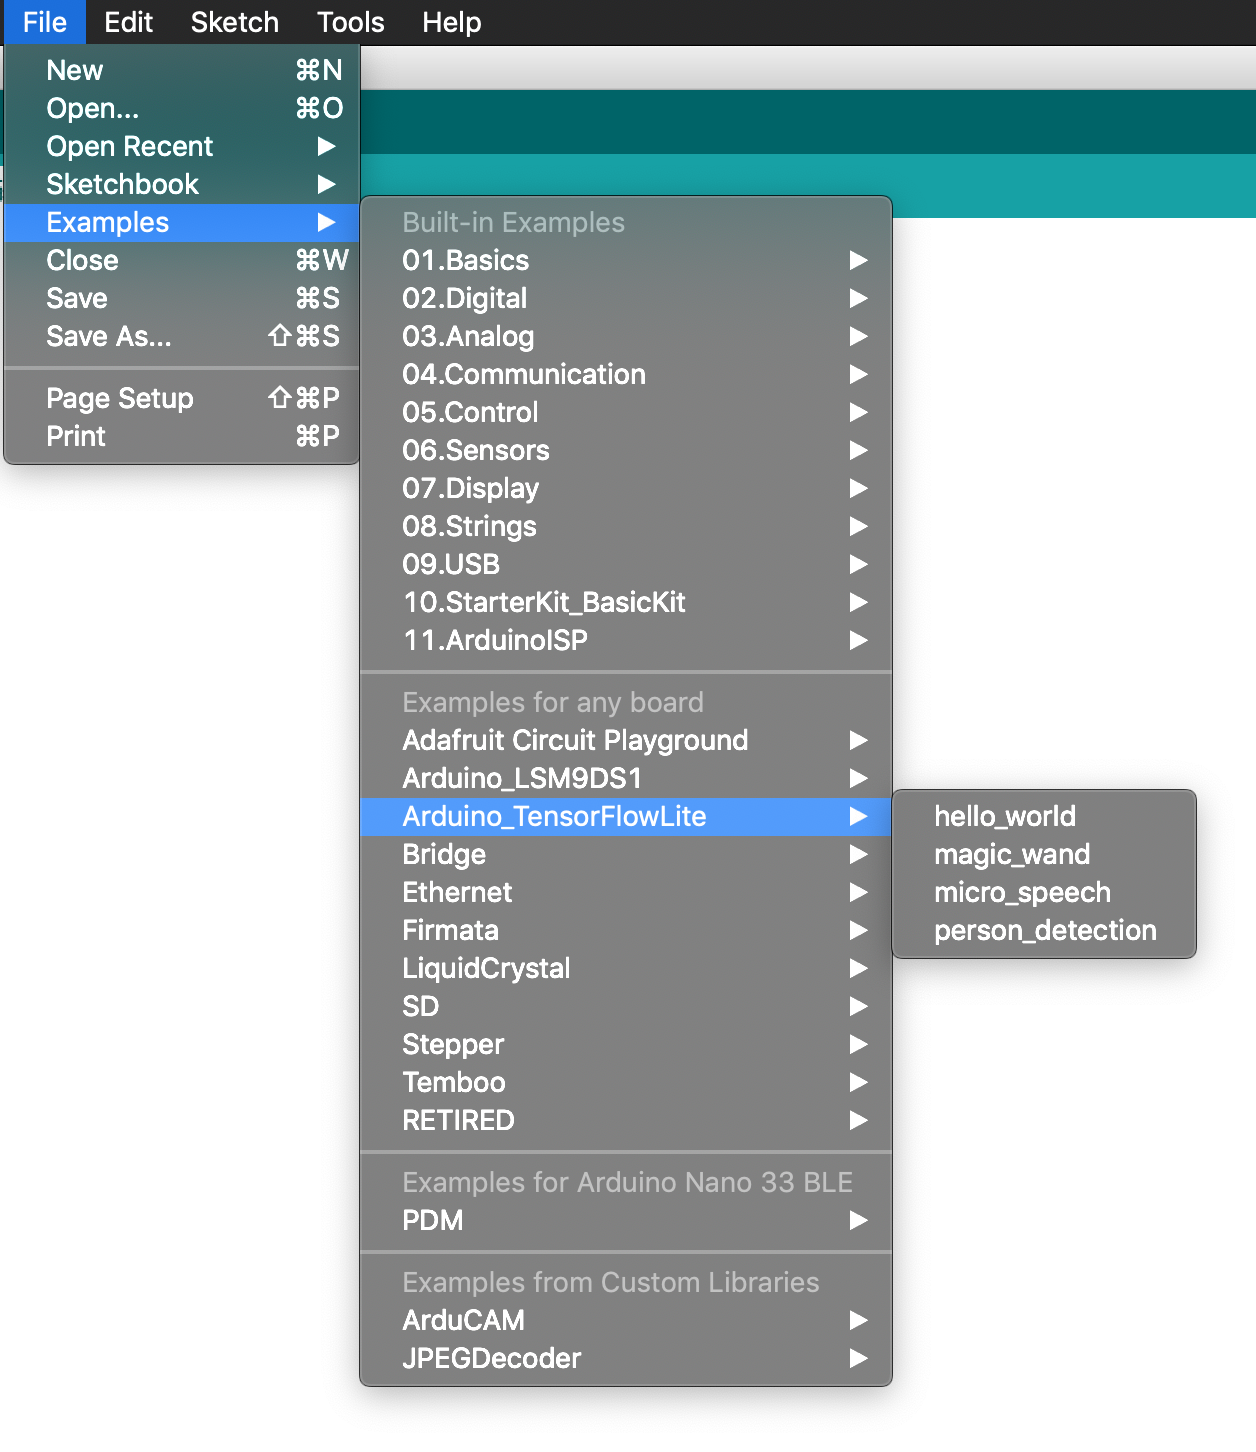
\includegraphics{Arduino/tinyML9-2}
  \caption{Screenshot des Menüs 'Examples'}\label{tinyML9-2}
\end{figure}



Klicken Sie auf \FILE{\glqq person\_detection\grqq}, um das Beispiel zu laden. Es erscheint ein neues Fenster mit einer Registerkarte für jede der Quelldateien. Die Datei in der ersten Registerkarte, \FILE{person\_detection}, entspricht der Datei \FILE{main\_functions.cc}, die wir zuvor durchgelesen haben.

\subsection{Bemerkung}

"Das Ausführen des Beispiels" hat bereits die Struktur des Arduino-Beispiels erklärt, daher werden wir es hier nicht noch einmal behandeln.

Zusätzlich zur TensorFlow-Bibliothek müssen wir zwei weitere Bibliotheken installieren:

\begin{enumerate}
  \item Die Bibliothek \FILE{Arducam}, damit unser Code mit der Hardware interagieren kann
  \item Die Bibliothek \FILE{JPEGDecoder}, damit wir JPEG-kodierte Bilder dekodieren können
\end{enumerate}

Die Arducam-Arduino-Bibliothek ist auf GitHub verfügbar. Um sie zu installieren, laden Sie das Repository herunter oder klonen Sie es. Kopieren Sie anschließend das Unterverzeichnis \FILE{ArduCAM} in Ihr Verzeichnis \FILE{Arduino/libraries}. Um das Bibliotheksverzeichnis auf Ihrem Rechner zu finden, überprüfen Sie den Sketchbook-Speicherort im Voreinstellungsfenster der Arduino IDE.

Nachdem Sie die Bibliothek heruntergeladen haben, müssen Sie eine ihrer Dateien bearbeiten, um sicherzustellen, dass sie für die Arducam Mini 2MP Plus konfiguriert ist. Öffnen Sie dazu \FILE{Arduino/libraries/ArduCAM/memorysaver.h}.

Sie sollten eine Reihe von \PYTHON{\#define}-Anweisungen aufgelistet sehen. Stellen Sie sicher, dass sie alle auskommentiert sind, außer \PYTHON{\#define OV2640\_MINI\_2MP\_PLUS}, wie hier gezeigt:

\begin{code}
    \begin{lstlisting}
//Step 1: select the hardware platform, only one at a time
//#define OV2640_MINI_2MP
//#define OV3640_MINI_3MP
//#define OV5642_MINI_5MP
//#define OV5642_MINI_5MP_BIT_ROTATION_FIXED
#define OV2640_MINI_2MP_PLUS
//#define OV5642_MINI_5MP_PLUS
//#define OV5640_MINI_5MP_PLUS
  \end{lstlisting}
\end{code}

Nachdem Sie die Datei gespeichert haben, sind Sie mit der Konfiguration der Arducam-Bibliothek fertig.

\subsection{Tip}

Das Beispiel wurde mit \SHELL{Commit \#e216049} der Arducam-Bibliothek entwickelt. Wenn Sie Probleme mit der Bibliothek haben, können Sie versuchen, diesen speziellen Commit herunterzuladen, um sicherzustellen, dass Sie genau denselben Code verwenden.

Der nächste Schritt ist die Installation der Bibliothek \FILE{JPEGDecoder}. Sie können dies aus der Arduino-IDE heraus tun. Wählen Sie im Menü "Tools" die Option "Manage Libraries" und suchen Sie nach \FILE{JPEGDecoder}. Sie sollten die Version 1.8.0 der Bibliothek installieren.

Nachdem Sie die Bibliothek installiert haben, müssen Sie sie konfigurieren, um einige optionale Komponenten zu deaktivieren, die nicht mit dem Arduino Nano 33 BLE Sense kompatibel sind. Öffnen Sie \FILE{Arduino/libraries/JPEGDecoder/src/User\_Config.h} und stellen Sie sicher, dass sowohl \PYTHON{\#define LOAD\_SD\_LIBRARY} als auch \PYTHON{\#define LOAD\_SDFAT\_LIBRAR} auskommentiert sind, wie in diesem Auszug aus der Datei gezeigt:

\begin{code}
    \begin{lstlisting}
// Comment out the next #defines if you are not using an SD Card to store
// the JPEGs
// Commenting out the line is NOT essential but will save some FLASH space if
// SD Card access is not needed. Note: use of SdFat is currently untested!

//#define LOAD_SD_LIBRARY // Default SD Card library
//#define LOAD_SDFAT_LIBRARY // Use SdFat library instead, so SD Card SPI can
// be bit bashed
  \end{lstlisting}
\end{code}

Nachdem Sie die Datei gespeichert haben, ist die Installation der Bibliotheken abgeschlossen. Sie sind nun bereit, die Anwendung zur Personenerkennung auszuführen!

Schließen Sie zunächst Ihr Arduino-Gerät über USB an. Vergewissern Sie sich, dass der richtige Gerätetyp in der Dropdown-Liste "Board" im Menü "Tools" ausgewählt ist, wie in Abbildung~\ref{tinyML9-3} gezeigt.

\begin{figure}
    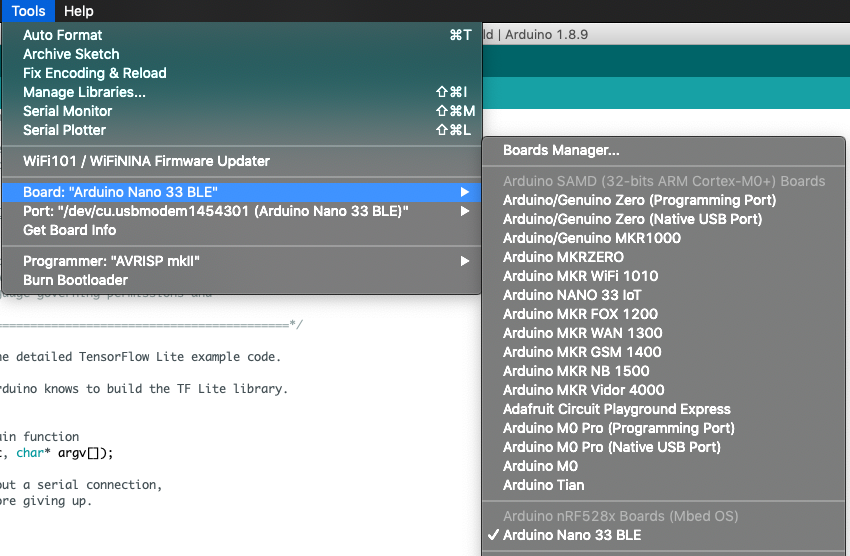
\includegraphics{Arduino/tinyML9-3}
    \caption{Screenshot of the 'Board' dropdown}\label{tinyML9-3}
\end{figure}


Wenn der Name Ihres Geräts nicht in der Liste erscheint, müssen Sie sein Support-Paket installieren. Klicken Sie dazu auf Boards Manager. Suchen Sie in dem daraufhin angezeigten Fenster nach Ihrem Gerät und installieren Sie die neueste Version des entsprechenden Support-Pakets.

Vergewissern Sie sich auch im Menü Tools, dass der Anschluss des Geräts in der Dropdown-Liste Port ausgewählt ist, wie in Abbildung~\ref{tinyML9-4} gezeigt.

\begin{figure}
    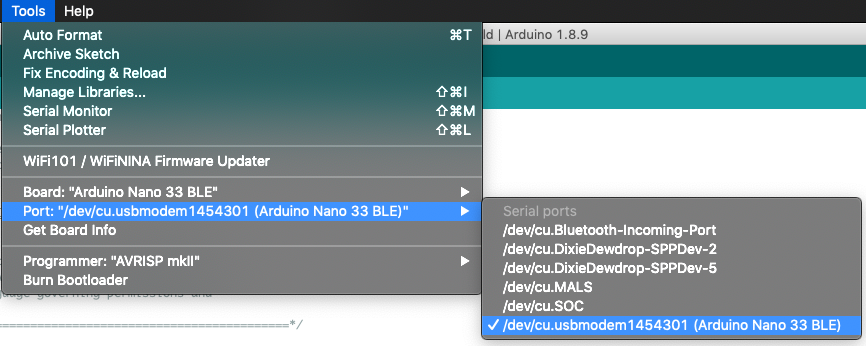
\includegraphics{Arduino/tinyML9-4}
    \caption{Screenshot of the 'Port' dropdown}\label{tinyML9-4}
\end{figure}


Klicken Sie schließlich im Arduino-Fenster auf die Schaltfläche "Hochladen" (in Abbildung~\ref{tinyML9-4} weiß hervorgehoben), um den Code zu kompilieren und auf Ihr Arduino-Gerät hochzuladen.


\begin{figure}
    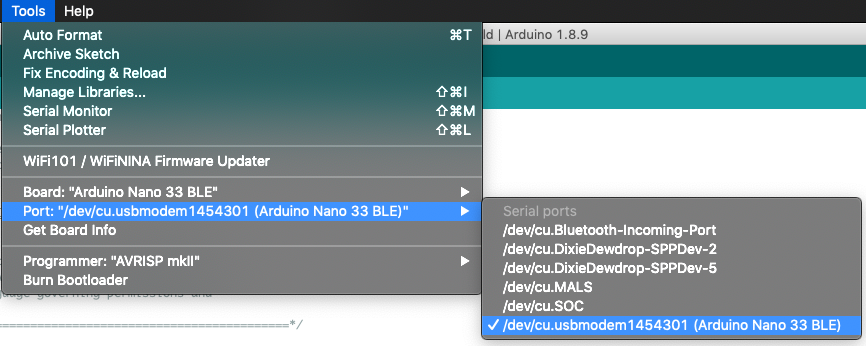
\includegraphics{Arduino/tinyML9-4}
    \caption{Screenshot of the upload button}\label{tinyML9-4}
\end{figure}

Sobald der Upload erfolgreich abgeschlossen ist, wird das Programm ausgeführt.

Um es zu testen, beginnen Sie damit, die Kamera des Geräts auf etwas zu richten, das definitiv keine Person ist oder nur das Objektiv verdeckt. Wenn die blaue LED das nächste Mal blinkt, nimmt das Gerät ein Bild von der Kamera auf und beginnt, die Inferenz auszuführen. Da das Bildverarbeitungsmodell, das wir für die Personenerkennung verwenden, relativ groß ist, wird die Inferenz sehr lange dauern - etwa 19 Sekunden zum Zeitpunkt des Schreibens, obwohl es möglich ist, dass TensorFlow Lite seitdem schneller geworden ist.

Wenn die Inferenz abgeschlossen ist, wird das Ergebnis in eine weitere leuchtende LED übersetzt. Sie haben die Kamera auf etwas gerichtet, das keine Person ist, also sollte die rote LED aufleuchten.

Versuchen Sie nun, die Kamera des Geräts auf sich selbst zu richten! Wenn die blaue LED das nächste Mal blinkt, nimmt das Gerät ein weiteres Bild auf und beginnt, die Inferenz durchzuführen. Nach etwa 19 Sekunden sollte die grüne LED aufleuchten.

Denken Sie daran, dass die Bilddaten vor jeder Inferenz als Schnappschuss aufgenommen werden, wenn die blaue LED blinkt. Das, worauf die Kamera in diesem Moment gerichtet ist, wird in das Modell eingespeist. Es spielt keine Rolle, worauf die Kamera gerichtet ist, bis das nächste Mal ein Bild aufgenommen wird, wenn die blaue LED wieder blinkt.

Wenn Sie scheinbar falsche Ergebnisse erhalten, stellen Sie sicher, dass Sie sich in einer Umgebung mit guter Beleuchtung befinden. Sie sollten auch sicherstellen, dass die Kamera richtig ausgerichtet ist, mit den Stiften nach unten, so dass die Bilder, die sie aufnimmt, richtig herum sind - das Modell wurde nicht darauf trainiert, auf dem Kopf stehende Personen zu erkennen. Außerdem sollten Sie bedenken, dass es sich um ein winziges Modell handelt, bei dem die Genauigkeit gegen die geringe Größe eingetauscht wird. Es funktioniert sehr gut, aber es ist nicht immer zu 100 % genau.

Sie können die Ergebnisse der Inferenz auch über den Arduino Serial Monitor sehen. Öffnen Sie dazu im Menü "Tools" den "Serial Monitor". Sie werden ein detailliertes Protokoll sehen, das zeigt, was passiert, während die Anwendung läuft. Es ist auch interessant, das Kästchen "Show timestamp" (Zeitstempel anzeigen) zu aktivieren, damit Sie sehen können, wie lange jeder Teil des Prozesses dauert:




\begin{code}
    \begin{lstlisting}
14:17:50.714 -> Starting capture
14:17:50.714 -> Image captured
14:17:50.784 -> Reading 3080 bytes from ArduCAM
14:17:50.887 -> Finished reading
14:17:50.887 -> Decoding JPEG and converting to greyscale
14:17:51.074 -> Image decoded and processed
14:18:09.710 -> Person score: 246 No person score: 66
  \end{lstlisting}
\end{code}

Aus diesem Protokoll ist ersichtlich, dass das Erfassen und Lesen der Bilddaten vom Kameramodul ca. 170 ms, das Dekodieren des JPEGs und die Umwandlung in Graustufen 180 ms und die Durchführung der Inferenz 18,6 Sekunden dauerte.

\subsection{Ausführung von Änderungen}

Jetzt, wo Sie die Basisanwendung bereitgestellt haben, können Sie ein wenig herumspielen und einige Änderungen am Code vornehmen. Bearbeiten Sie einfach die Dateien in der Arduino-IDE und speichern Sie sie, und wiederholen Sie dann die vorherigen Anweisungen, um den geänderten Code auf dem Gerät einzusetzen.

Hier sind ein paar Dinge, die Sie ausprobieren können:

\begin{itemize}
  \item Ändern Sie den Erkennungsresponder so, dass er mehrdeutige Eingaben ignoriert, bei denen es keinen großen Unterschied zwischen den Bewertungen "Person" und "keine Person" gibt.
\item Verwenden Sie die Ergebnisse der Personenerkennung, um andere Komponenten zu steuern, z. B. zusätzliche LEDs oder Servos.
\item Bauen Sie eine intelligente Sicherheitskamera, indem Sie Bilder speichern oder übertragen - aber nur solche, die eine Person enthalten.
\end{itemize}





















\cite{Chowdhery:2019}


\url{https://github.com/tensorflow/tensorflow/tree/master/tensorflow/lite/micro/examples/person\_detection}

\subsection{Laufen auf Arduino}

Die folgenden Anweisungen helfen Ihnen, dieses Beispiel zu erstellen und auf Arduino-Geräten einzusetzen.

Das Beispiel wurde mit dem folgenden Gerät getestet:

Arduino Nano 33 BLE Sense
Sie benötigen außerdem das folgende Kameramodul:

Arducam Mini 2MP Plus

Hardware
Schließen Sie die Pins der Arducam wie folgt an:

\begin{tabular}{ll}
  Arducam pin name & Arduino pin name \\ \hline
  CS               & D7 (unlabelled, immediately to the right of D6) \\
  MOSI             & D11 \\
  MISO             & D12 \\
  SCK              & D13 \\
  GND              & GND (either pin marked GND is fine) \\
  VCC              & 3.3 V \\
  SDA              & A4 \\
  SCL              & A5 \\
\end{tabular}

Installieren Sie die Bibliothek \FILE{Arduino\_TensorFlowLite}

Laden Sie den aktuellen nächtlichen Build der Bibliothek herunter: \FILE{person\_detection.zip}

Diese Beispielanwendung ist als Teil der offiziellen TensorFlow Lite Arduino-Bibliothek enthalten. Um sie zu installieren, öffnen Sie den Arduino Bibliotheksmanager in Tools -> Manage Libraries... und suchen Sie nach \FILE{Arduino\_TensorFlowLite}.

\subsection{Installation anderer Bibliotheken}

Zusätzlich zur TensorFlow-Bibliothek müssen Sie noch zwei weitere Bibliotheken installieren:

Die Arducam-Bibliothek, damit unser Code mit der Hardware kommunizieren kann
Die JPEGDecoder-Bibliothek, so dass wir JPEG-kodierte Bilder dekodieren können
Die Arducam-Arduino-Bibliothek ist auf GitHub unter \url{https://github.com/ArduCAM/Arduino} verfügbar. Um sie zu installieren, laden Sie das Repository herunter oder klonen Sie es. Kopieren Sie anschließend das Unterverzeichnis ArduCAM in Ihr Arduino/libraries-Verzeichnis. Um dieses Verzeichnis auf Ihrem Rechner zu finden, überprüfen Sie den Sketchbook-Speicherort im Fenster "Einstellungen" der Arduino IDE.

Nachdem Sie die Bibliothek heruntergeladen haben, müssen Sie eine ihrer Dateien bearbeiten, um sicherzustellen, dass sie für die Arducam Mini 2MP Plus konfiguriert ist. Öffnen Sie dazu die folgende Datei:

\FILE{Arduino/libraries/ArduCAM/memorysaver.h}

You'll see a bunch of \PYTHON{\#define} statements listed. Make sure that they are all commented out, except for \PYTHON{\#define OV2640\_MINI\_2MP\_PLUS}, as so:

\begin{code}
    \begin{lstlisting}
//Step 1: select the hardware platform, only one at a time
//#define OV2640_MINI_2MP
//#define OV3640_MINI_3MP
//#define OV5642_MINI_5MP
//#define OV5642_MINI_5MP_BIT_ROTATION_FIXED
#define OV2640_MINI_2MP_PLUS
//#define OV5642_MINI_5MP_PLUS
//#define OV5640_MINI_5MP_PLUS
  \end{lstlisting}
\end{code}

Sobald Sie die Datei gespeichert haben, sind wir mit der Konfiguration der Arducam-Bibliothek fertig.

Unser nächster Schritt ist die Installation der JPEGDecoder-Bibliothek. Wir können dies aus der Arduino-IDE heraus tun. Gehen Sie zunächst auf die Option "Manage Libraries..." im Menü "Tools" und suchen Sie nach JPEGDecoder. Sie sollten die Version 1.8.0 der Bibliothek installieren.

Sobald die Bibliothek installiert ist, müssen wir sie konfigurieren, um einige optionale Komponenten zu deaktivieren, die nicht mit dem Arduino Nano 33 BLE Sense kompatibel sind. Öffnen Sie die folgende Datei:

\FILE{Arduino/libraries/JPEGDecoder/src/User\_Config.h}

Stellen Sie sicher, dass sowohl \PYTHON{\#define LOAD\_SD\_LIBRARY} als auch \PYTHON{\#define LOAD\_SDFAT\_LIBRARY} auskommentiert sind, wie in diesem Auszug aus der Datei gezeigt:


\begin{code}
    \begin{lstlisting}
// Comment out the next #defines if you are not using an SD Card to store the JPEGs
// Commenting out the line is NOT essential but will save some FLASH space if
// SD Card access is not needed. Note: use of SdFat is currently untested!

//#define LOAD_SD_LIBRARY // Default SD Card library
//#define LOAD_SDFAT_LIBRARY // Use SdFat library instead, so SD Card SPI can be bit bashed-device, then build and upload the example.
  \end{lstlisting}
\end{code}



Um die Kamera zu testen, beginnen Sie damit, die Kamera des Geräts auf etwas zu richten, das definitiv keine Person ist, oder sie einfach zu verdecken. Wenn die blaue LED das nächste Mal blinkt, erfasst das Gerät ein Bild von der Kamera und beginnt mit der Inferenz. Das Bildverarbeitungsmodell, das wir für die Personenerkennung verwenden, ist relativ groß, aber mit den cmsis-nn-Optimierungen dauert es nur etwa 800 ms, um das Modell auszuführen.

Nach einem Moment wird das Ergebnis der Inferenz in das Aufleuchten einer weiteren LED umgesetzt. Da Sie die Kamera auf etwas gerichtet haben, das keine Person ist, sollte die rote LED aufleuchten.

Versuchen Sie nun, die Kamera des Geräts auf sich selbst zu richten! Wenn die blaue LED das nächste Mal blinkt, nimmt das Gerät ein weiteres Bild auf und beginnt, die Inferenz durchzuführen. Nach einer kurzen Pause sollte die grüne LED aufleuchten!

Denken Sie daran, dass die Bilddaten vor jeder Inferenz als Schnappschuss aufgenommen werden, wenn die blaue LED blinkt. Das, worauf die Kamera in diesem Moment gerichtet ist, wird in das Modell eingespeist. Es spielt keine Rolle, wohin die Kamera gerichtet ist, bis das nächste Mal ein Bild aufgenommen wird, wenn die blaue LED wieder blinkt.

Wenn Sie scheinbar falsche Ergebnisse erhalten, stellen Sie sicher, dass Sie sich in einer Umgebung mit guter Beleuchtung befinden. Sie sollten auch sicherstellen, dass die Kamera richtig ausgerichtet ist, mit den Stiften nach unten, so dass die Bilder, die sie aufnimmt, richtig herum sind - das Modell wurde nicht darauf trainiert, auf dem Kopf stehende Personen zu erkennen! Außerdem sollte man bedenken, dass es sich um ein winziges Modell handelt, bei dem die Genauigkeit gegen die geringe Größe eingetauscht wird. Es funktioniert sehr gut, aber es ist nicht immer zu 100 % genau.

Wir können die Ergebnisse der Inferenz auch über den Arduino Serial Monitor sehen. Dazu öffnen Sie den Serial Monitor aus dem Menü Tools. Sie werden ein detailliertes Protokoll dessen sehen, was passiert, während unsere Anwendung läuft. Es ist auch interessant, das Kontrollkästchen Zeitstempel anzeigen zu aktivieren, so dass Sie sehen können, wie lange jeder Teil des Prozesses dauert:



\begin{code}
    \begin{lstlisting}
14:17:50.714 -> Starting capture
14:17:50.714 -> Image captured
14:17:50.784 -> Reading 3080 bytes from ArduCAM
14:17:50.887 -> Finished reading
14:17:50.887 -> Decoding JPEG and converting to greyscale
14:17:51.074 -> Image decoded and processed
14:18:09.710 -> Person score: 246 No person score: 66
  \end{lstlisting}
\end{code}

Aus dem Protokoll geht hervor, dass etwa 170 ms für die Erfassung und das Lesen der Bilddaten vom Kameramodul, 180 ms für die Dekodierung des JPEGs und die Umwandlung in Graustufen und 18,6 Sekunden für die Inferenz benötigt wurden.


\chapter{Hardware the Arduino Nano 33 BLE Sense}

\section{Indroduction}

Arduino has a wide range of Integrated circuit family, depending upon the requirenment and usage. The most commonly available arduino family boards are MKR Family, Arduino Classis, Nano fmaily, Pro Family, and Nicla Family. Each arduino family have further multiple types of boards, e.g the Nano family has a following boards; Nano Classic, Nano 33 BLE, Nano 33 BLE Sense, Nano 33 IoT, and Nano Every, each has a unique specification. The Arduino development board is based on a microcontroller with a large number of standard electronic components and an open source schematic that can be modified as needed.

The BLE (Bluetooth Low Energy) compact and reliable Nano board are built on NINA B306 module for BLE and Bluetooth 5 communication; the NINA B306 module based on Nordic nRF52480 processor that contains a powerful Cortex M4F CPU, Its architecture fully compatible with Arduino IDE Online and Offline. The figure ~\ref{fig:abx00031front12} shows, the Arduino Nano BLE 33 Sense have a following set of sensors on board, ADPS-9960, LPS22HB, HTS221, LSM9DS1,and MP34DT05-A. It is small in size, having all the required sensor on board. \cite{ArduinoNano33:2021}



\begin{figure}[ht]
	\centering
	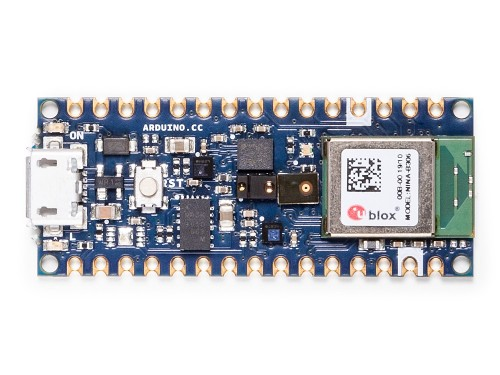
\includegraphics[width=0.5\linewidth]{Nano33BLESense/abx00031_front_1_2}
	\caption{Arduino Nano 33 BLE}
	\label{fig:abx00031front12}
\end{figure}

The Arduino Nano 33 BLE Sense have the following set of Sensors, BLE module and its functionality below.

\begin{itemize}
	\item The Bluetooth is managed by a NINA B306 module.
	\item The ADPS-9960 is a digital proximity, ambient light, RGB and gesture sensor.
	\item The LSM9DS1 is a system-in-package featuring a 3D digital linear acceleration sensor, a 3D digital angular rate sensor, and a 3D digital magnetic sensor.
	\item The LPS22HB reads barometric pressure and environmental temperature.
	\item The HTS221 senses relative humidity.
	\item The MP34DT05 is support the sound detection.
\end{itemize}

\section{On Board Sensors and its Functionality}

\subsection{ADPS-9960 (Gesture, Proximity, and Color Detection Sensor)}

The APDS-9960 device features advanced Gesture detection, Proximity detection, Digital Ambient Light Sense (ALS) and Color Sense (RGB). \cite{ArduinoNano33:2021} Gesture detection utilizes four directional photodiodes to sense reflected IR energy (sourced by the integrated LED) to convert physical motion information (i.e. velocity, direction and distance) to a digital information.



\textbf{Applications}

\begin{itemize}
  \item Gesture Detection
  \item Color Sense
  \item Ambient Light Sensing
  \item Proximity Sensing
\end{itemize}

\subsection{LSM9DS1 (Accelerometer, Gyroscope, and Magnetometre)}
The LSM9DS1 is a system-in-package featuring a 3D digital linear acceleration sensor, a 3D digital angular rate sensor, and a 3D digital magnetic sensor.

\textbf{Aplications}

\begin{itemize}
  \item Indoor navigation
  \item Advanced gesture recognition
  \item Gaming and virtual reality input devices
  \item Display/map orientation and browsing
\end{itemize}
  
\subsection{LPS22HB (Pressure Sensor)}
The LPS22HB is an ultra-compact piezoresistive absolute pressure sensor which functions as a
digital output barometer.

\textbf{Applications}


\begin{itemize}
  \item Altimeters and barometers for portable devices 
  \item Weather station equipment
  \item Sports watchs
\end{itemize}

\subsection{HTS221 (Relative Humidity and Temperature)}
The HTS221 is an ultra-compact sensor for relative humidity and temperature. It includes a sensing element and a mixed signal to provide the measurement information through digital serial interfaces.

\textbf{Applications}

\begin{itemize}
  \item Air conditioning, heating and ventilation 
  \item Air humidifiers
  \item Refrigerators
  \item Smart home automation
  \item Industrial automation
\end{itemize}  


\subsection{MP34DT05-A (Digital Microphone)}

The MP34DT05-A is an ultra-compact, low-power, omni directional, digital microphone built with a capacitive sensing element and an IC interface. The sensing element, capable of detecting acoustic waves, is manufactured using a specialized silicon micromachining process dedicated to producing audio sensors.

\textbf{Applications}

\begin{itemize}
  \item Speech recognition 
  \item Portable media player
  \item Mobile Terminal
\end{itemize}


\subsection{nRF52840 (Bluetooth Module)}

The nRF52840 is an advanced, highly flexible single chip solution for today’s increasingly demanding Ultra low power (ULP) wireless applications for connected devices on our person, connected living environments and the IoT at large. It is designed ready for the major feature
advancements of Bluetooth 5 and takes advantage of Bluetooth 5’s increased performance capabilities. \cite{Arduino:2021b}

\textbf{Applications}

\begin{itemize}
  \item Smart Home products
  \item Industrial mesh networks
  \item Smart city infrastructure
  \item Connected watches
  \item Advanced personal fitness devices
  \item Wearables with wireless payment
  \item Connected Health
\end{itemize}

The Arduino 33 BLE Sense has a wide range of application, by having the set of sensors and Bluetooth low energy (BLE) capability, the communication becomes easy over the Bluetooth. Arduino Nano 33 BLE Sense operate on 3.3 V, so it make sure that do not apply 5v as normally the other boards need to operate. Also, for making the RGB color and person detection, we need to make the interface of Ble 33 Sense with Arducam OV2640 (Camera Shield). The Arducam OV2640 camera use  to detect the RGB, object detetion and also the gesture too. Arduino Nano 33 BLE Sense and Arducam (camera shield) is a perfect mactch for making ML and AI application, by having the set of sensors on board we just need to install the respective library on Arduino boar and it support the funcnality of sensors and Machine learning application.

\section{Arduino Nano 33 BLE Pin Configuration}

Arduino Nano 33 BLE is an advanced version of Arduino Nano board that is based on a powerful processor the nRF52840. The figure ~\ref{Schnittstellen} shows that the board has the following pin configuration. \href{https://www.etechnophiles.com/arduino-nano-33-ble-sense-pinout-introduction-specifications/}{Pin Configuration}

\textbf{Digital pin:}

The number of digital I/O pins are 14 which receive only two values HIGH or LOW. These pins can either be used as an input or output based on the requirement. When these pins receive 5V, they are in a HIGH state and when they receive 0V they are in a LOW state.

\textbf{Analog pin}

Total 8 analog pins available on the board A0 – A7. These pins get any value as opposed to digital pins that only receive two values HIGH or LOW. These pins are used to measure the analog voltage ranging between 0 to 5V.


\textbf{PWM pin}

All digital pins can be used as PWM pins. These pins generate analog results with digital means.


\textbf{SPI pin}

The board supports serial peripheral interface (SPI) communication protocol. This protocol is employed to develop communication between a controller and other peripheral devices like shift registers and sensors. Two pins are used for SPI communication i.e. Master Input Slave Output (MISO) and Master Output Slave Input (MOSI) are used for SPI communication. These pins are used to send or receive data by the controller.

\textbf{I2C pin}

The board carries the I2C communication protocol which is a two-wire protocol. It comes with two pins SDL and SCL.

\textbf{UART pin}

The board features a UART communication protocol that is used for serial communication and carries two pins Rx and Tx. The Rx is a receiving pin used to receive the serial data while Tx is a transmission pin used to transmit the serial data.


\textbf{External Interrupts pin}

All digital pins can be used as external interrupts. This feature is used in case of emergency to interrupt the main running program with the inclusion of important instructions at that point.

\textbf{LED at Pin 13 and AREF pin}

There is an LED connected to pin 13 of the board. And AREF is a pin used as a reference voltage for the input voltage.



\begin{figure}[ht]
	\centering
	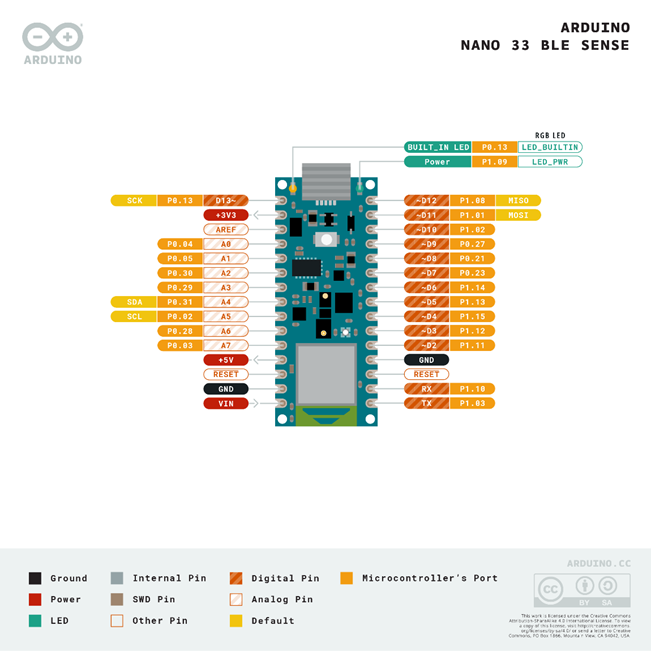
\includegraphics[width=0.5\linewidth]{Nano33BLESense/Schnittstellen}
	\caption{Arduino Nano 33 BLE Pin Configuration}
	\label{Schnittstellen}
\end{figure}


\chapter{ArduCAM OV2640}

\section{Indroduction}

ArduCAM is Arduino based open source camera platform which is well mated to Arduino boards. It is a high definition 2MP SPI camera, which reduce the complexity of the camera control interface. It integrates 2MP CMOS image sensor OV2640, and provides miniature size, as well as the easy to use hardware interface and open source code library. The ArduCAM mini can be used in any platforms like Arduino, Raspberry Pi, Maple, Chipkit, Beaglebone black, as long as they have SPI and I2C interface and can be well mated with standard Arduino boards. The figure ~\ref{Arducam} shows the mini ArduCAM Camera. The mini ArduCAM OV2640 is well suited for tinyML application, it is easy to configure with Arduino boards. For making the ML applications, especially Images caputuring, object and gesture detection, it supports to take capture and send back to Arduino microcontroller for getting desire results. \href{https://www.arducam.com/product/arducam-2mp-spi-camera-b0067-arduino/}{[Arducam]}

\begin{figure}[ht]
	\centering
	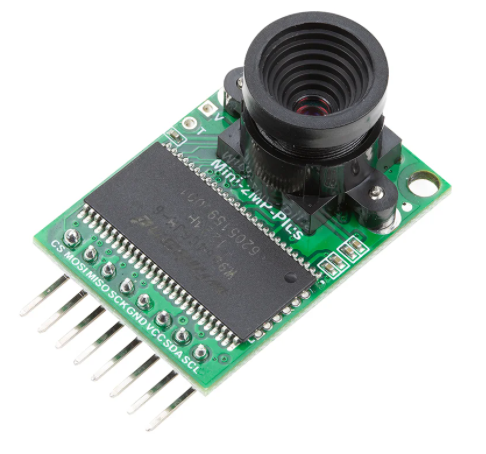
\includegraphics[width=0.5\linewidth]{Nano33BLESense/Arducam 2}
	\caption{ArduCAM interface with Arduino}
	\label{Arducam}
\end{figure}

\subsection{Pin Configuration of Arducam 0V2640 2MP Mini}

Arducam Mini 2MP OV2640 is a small mini size camera, we can easily embed this camera with any kind of Arduino or other electronics boards, if they have the serial peripheral interface (SPI) and  chip select (CS) . It has has 8 pins, the following figure ~\ref{pin config} shows the functionality of each pin.

\begin{figure}[ht]
	\centering
	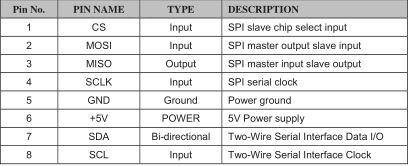
\includegraphics[width=0.8\linewidth]{Nano33BLESense/pin config}
	\caption{ArduCAM Pin Config}
	\label{pin config}
\end{figure}

It offers to add a camera interface with microcontroller the one who dont have camera capability, also there is a option to add multiple cameras with microcontroller.

\section{ArduCAM Interface with Arduino}

ArduCAM OV2640 needs the  SPI and I2C connection with the arduino boards. It will be connecting untill these two connections are make sure. The figure ~\ref{1} shows the ArduCAM connection with Arduino Mega 2560, the same connection will need with the other arduino boards too untill the availabity of  SPI and I2C connection. These ArduCAM cameras are easy to configure with arduino and depends upon the application, it is possible to connect multiple camera with sigle board to make the edge computing application. \href{https://www.arducam.com/product/arducam-2mp-spi-camera-b0067-arduino/}{Arducam Interface}

\begin{figure}[ht]
	\centering
	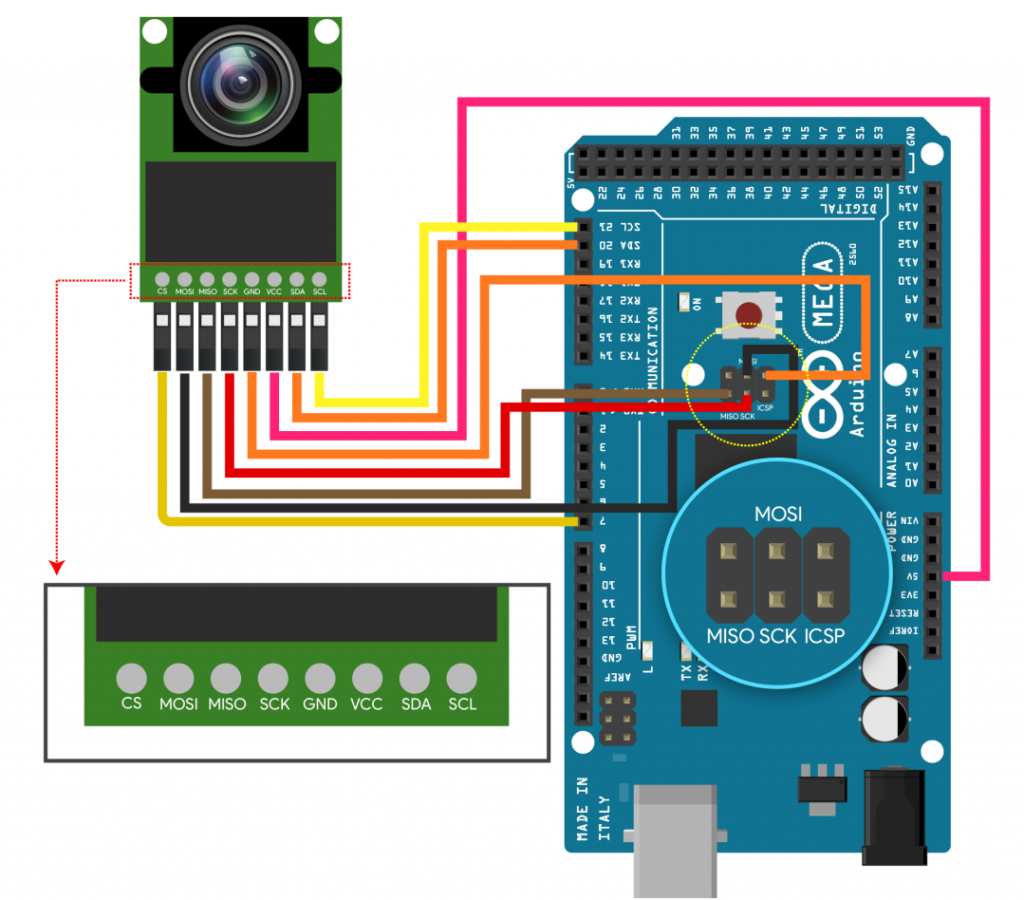
\includegraphics[width=0.6\linewidth]{Nano33BLESense/1}
	\caption{ArduCAM Interface with Arduin Mega 2560} 
	\label{1}
\end{figure}

ArduCAM is very small in size, even it is possible to fix the camera on the Arduino board. There is no external battery require for ArduCam to operate, It needs 5V/70mA operating power supply, so it will get the power from the arduino board too. By having the innovative funcnality with arduino boards, this can be use in the following applications.

\textbf{Application}

\begin{itemize}
  \item IOT Cameras
  \item Robot Cameras
  \item Wildlife Cameras
\end{itemize}  


\chapter{Software}

\section{Arduino IDE on PC}

\subsection{Installation}

Arduino Nano 33 BLE Sense can provide an energy-efficient and cost-effective solution for manufacturers who want to use Bluetooth Low Energy connectivity in their projects.\\

Arduino Nano 33 BLE Sense uses the Arduino software integrated development environment (IDE) for programming, which is the most widely used and common (IDE) for all arduino boards that can be run online and offline. This is a open-source Arduino Software (IDE) makes it easy to write code and upload it to the board. There are various version of software which is supported for each operating system (OS) e.g: mac, linux, and windows. Arduino community also provide us to start coding online and save our sketches in the cloud, this online arduino editor is most up-to-date version of the IDE includes all libraries and also supports new Arduino boards. For getting access to these software packages go to the following link \url{https://www.arduino.cc/en/software}  and get more up to date inforamtion, because every single day there are some updates occurs which is available on the link mention above. These software can be used with any Arduino board, the most recent offline arduino IDE 1.8.15 can be seen in Figure, \ref{fig:arduino-creat-agent-installieren} it is also supportive for all operating systems.

\begin{figure}[h]
	\centering
	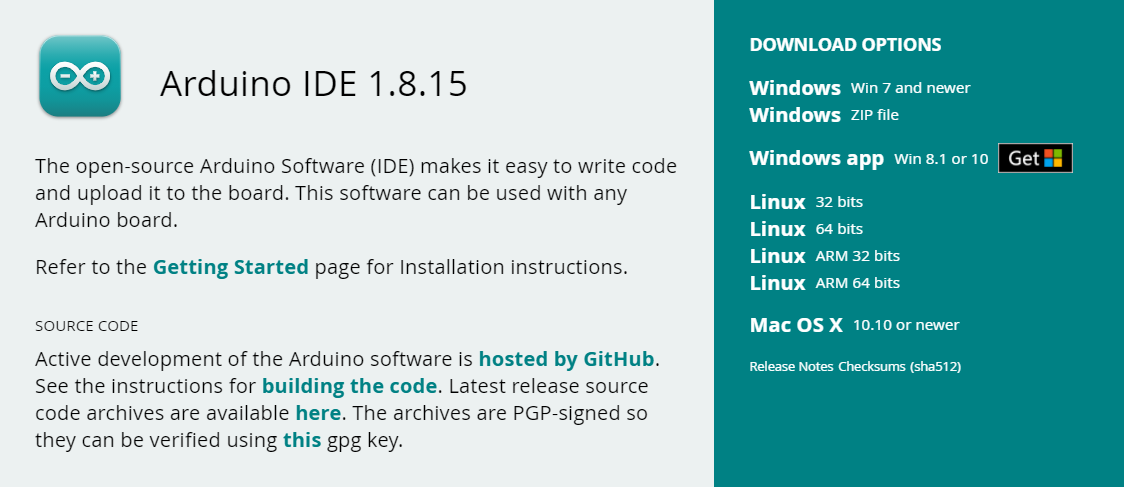
\includegraphics[width=1.0\linewidth]{Nano33BLESense/Installation-1}
	\caption{Arduino Creat Agent Installation}
	\label{fig:arduino-creat-agent-installieren}
\end{figure}


\subsection{Configuration}

To program the Arduino Nano 33 BLE Sense in offline state, we need to install one of the latest arduino IDE on our desktop. After installation, for getting access to the Arduino nano 33 ble sense board, we need to make configuration in our IDE. By opening the IDE, go to tool which can be seen on the uper left corner in IDE, in the tool there is an option for managed board. At this point we need to write our board name in the search which is Arduino Nano 33 BLE Sense as shown in figure, \ref {fig:Arduino-Mbed-Boards Installation} select the Arduino Mbed OS Boards and install it. The Mbed OS nano board supports also other nano family boards including Arduino nano 33 ble sense, after installing simply connect the Arduino Nano 33 BLE Sense to the computer via USB cable. 

\begin{figure}[h]
	\centering
	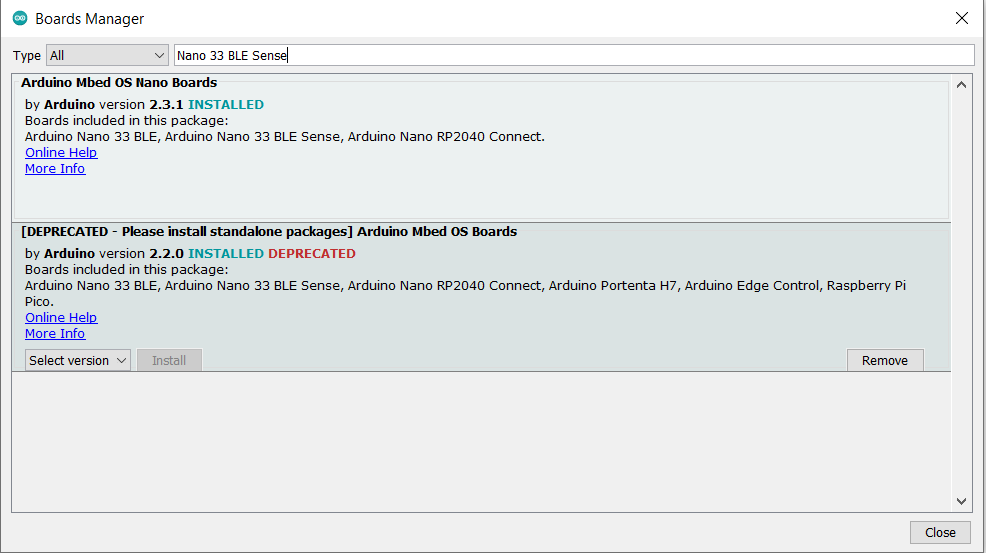
\includegraphics[width=1.0\linewidth]{Nano33BLESense/Nano Mbed}
	\caption{Arduino Mbed OS Nano Boards Installation}
	\label{fig:Arduino-Mbed-Boards Installation}
\end{figure}


\subsection{Test Example}

There are set of examples which are build in Arduino (IDE) for the testing purpose, for checking all the configuration and setting up the board we can open one of the basic LED blink example first as shown in the figure.  \ref{fig:LED-Example}.

\begin{figure}[h]
	\centering
	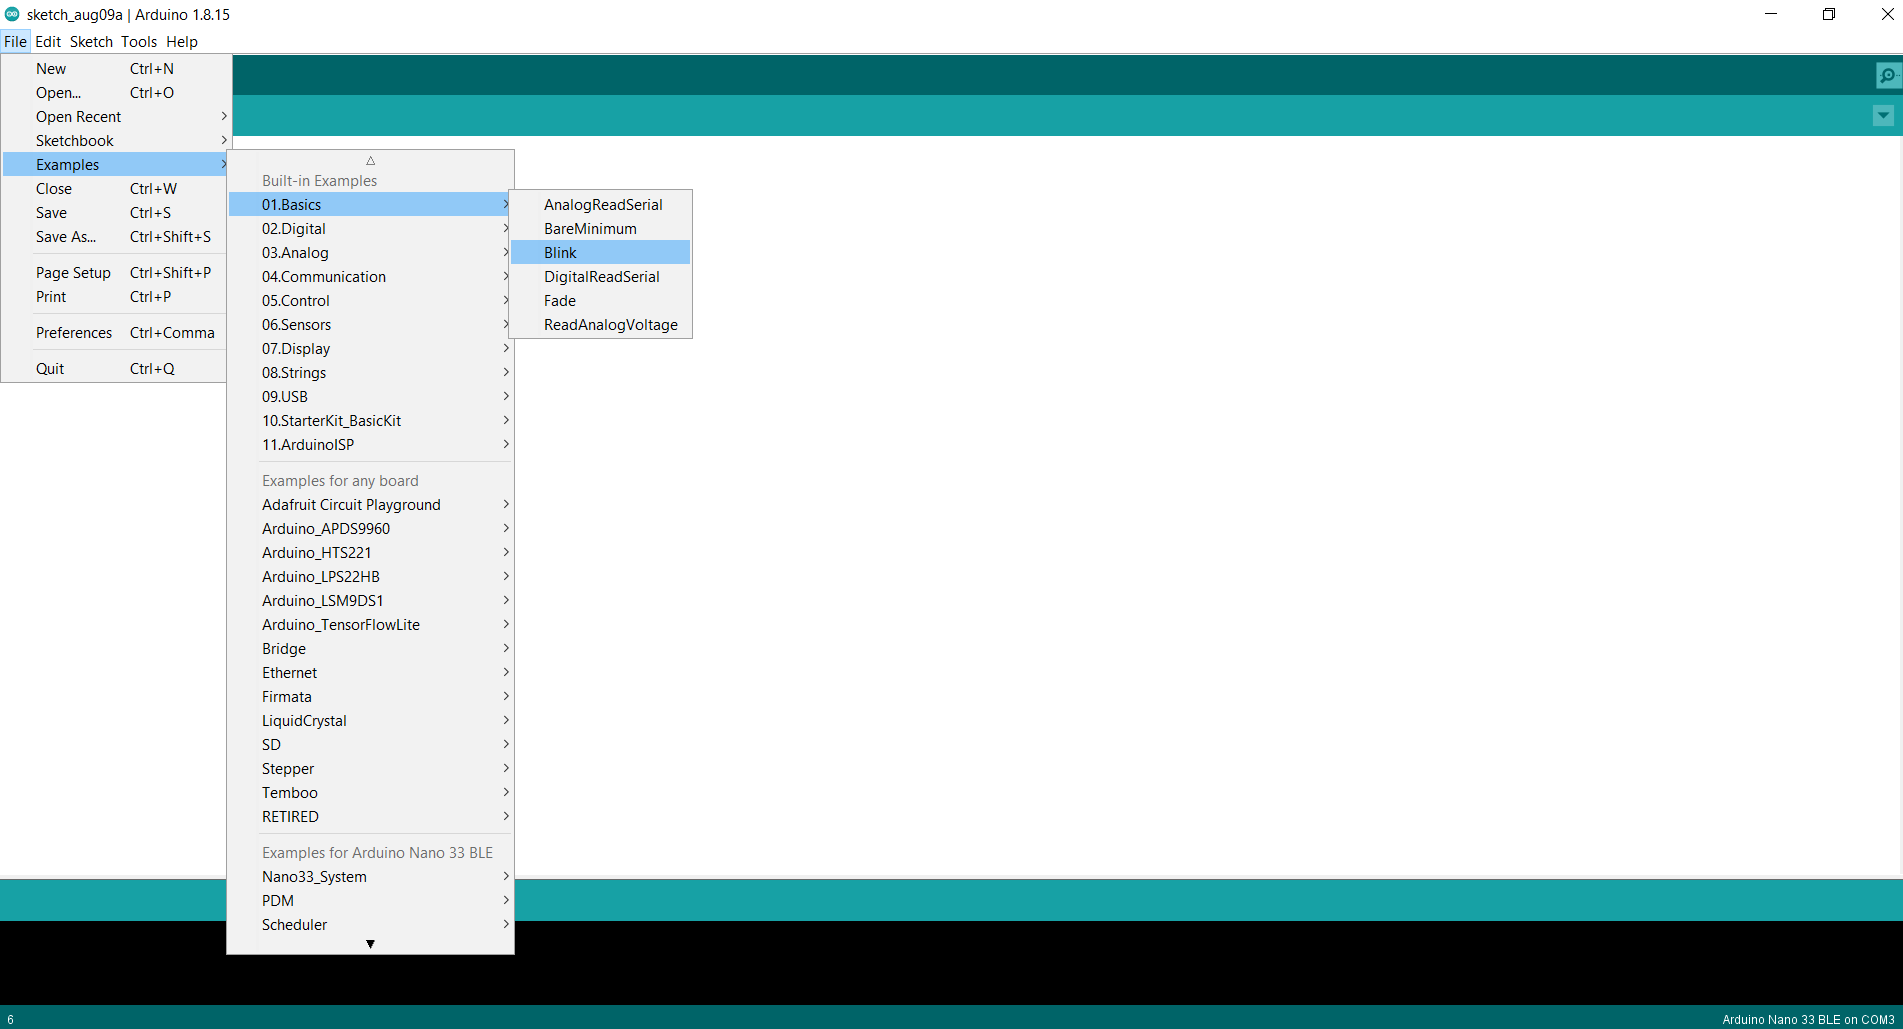
\includegraphics[width=1.0\linewidth]{Nano33BLESense/LED}
	\caption{LED-Example Test}
	\label{fig:LED-Example}
\end{figure}

This LED-blink example support all the arduino boards, for the checking purposes just need to run this basic example on any arduino embed board and it will blink the LED on our Arduino board after pre-set miliseconds. In the same example folder, there are also number of build in usefull example written in Arduino IDE for embedded boards. These examples are very usefull for getting the basic knowledge about the board and programming.

\section{Pre-requisite settings for Uploading the program}

There are some pre-requisite steps need to follow either we need to run the build in example or run by our own written program. By operating the Arduino board with Laptop with the help of USB connection, need to open the Arduino IDE on desktop, it appears a blank arduino environment page just a Void setup and void loop written on it. At this step we need to go to the tool-Arduino board and select the connected board which is Arduino Nano 33 Ble Sense as shown in the figure \ref{fig:Check Board}

\begin{figure}[h]
	\centering
	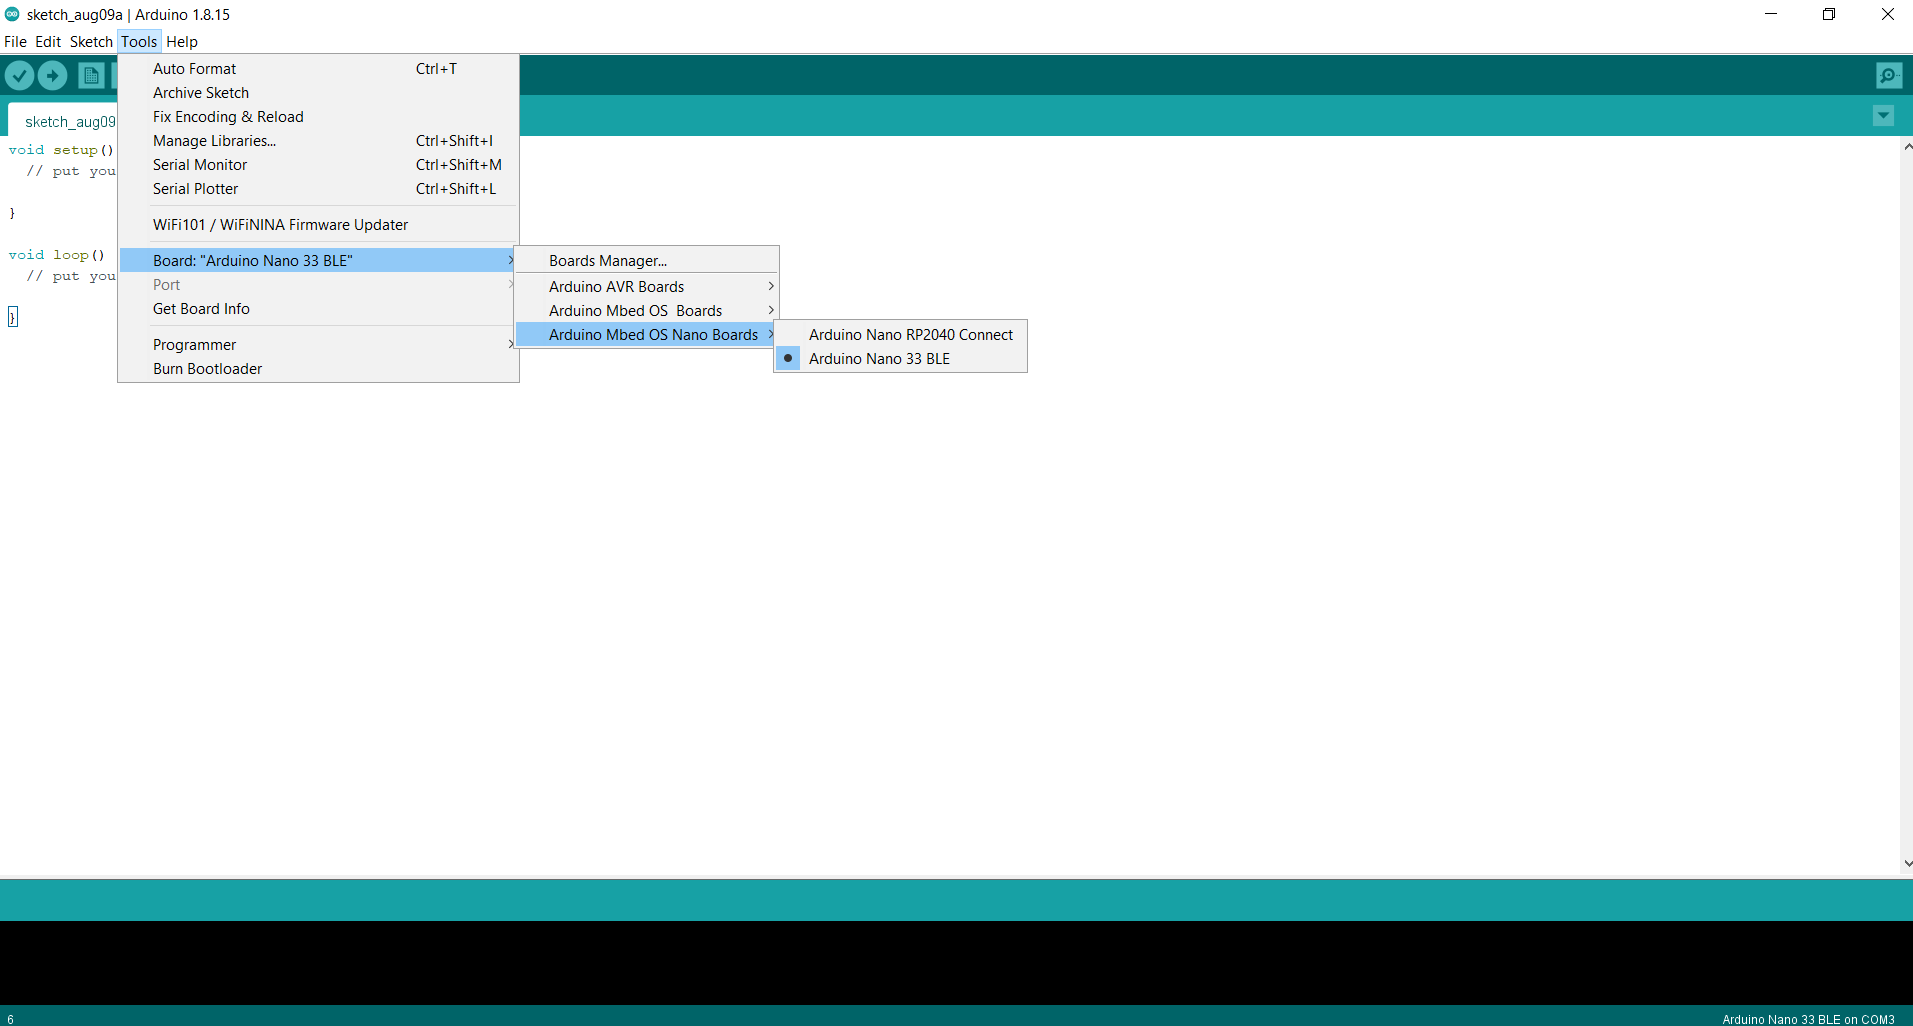
\includegraphics[width=1.0\linewidth]{Nano33BLESense/Check-board}
	\caption{Select the Connected board}
	\label{fig:Check Board}
\end{figure}

\subsection{Select the Appropriate Port}

By selecting the Arduino nano 33 BLE sense board, next we need to check the connected port. For doing this, we need to set our arduino borad in Boot setup by clicking the white reset button on arduino as show in figure\ref{fig:Check-Reset}.

\begin{figure}[h]
	\centering
	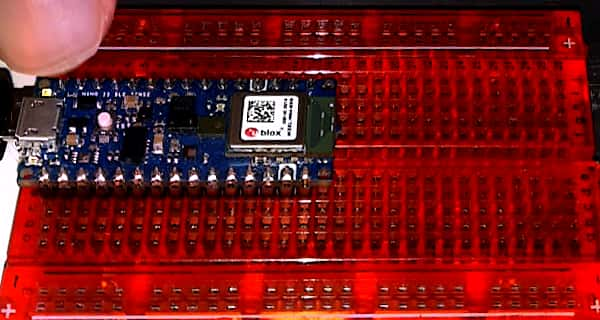
\includegraphics[width=1.0\linewidth]{Nano33BLESense/Click-Reset}
	\caption{Reset Button}
	\label{fig:Check-Reset}
\end{figure}

By clicking the white reset button, the arduino borad will be in boot setup and make sure to check the orange LED glow as shown in the figure \ref{fig:LED-Glow}.

\begin{figure}[h]
	\centering
	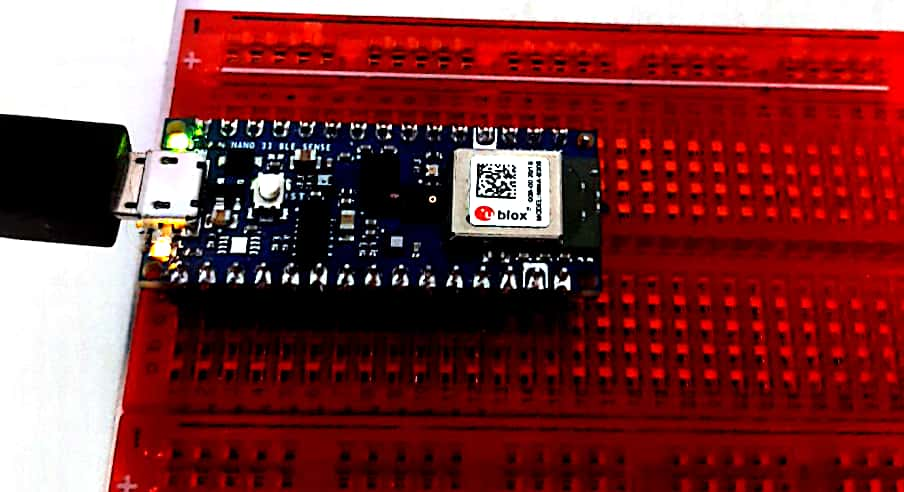
\includegraphics[width=1.0\linewidth]{Nano33BLESense/Orange LED}
	\caption{Orange LED Glow}
	\label{fig:LED-Glow}
\end{figure}

After successfully applying the above mention step, next we need to select the connected port before upload the program. For this, go to tool select arduino port and make sure to check it available port for uploading the program as shown in figure \ref{fig:Port-Selection}

\begin{figure}[h]
	\centering
	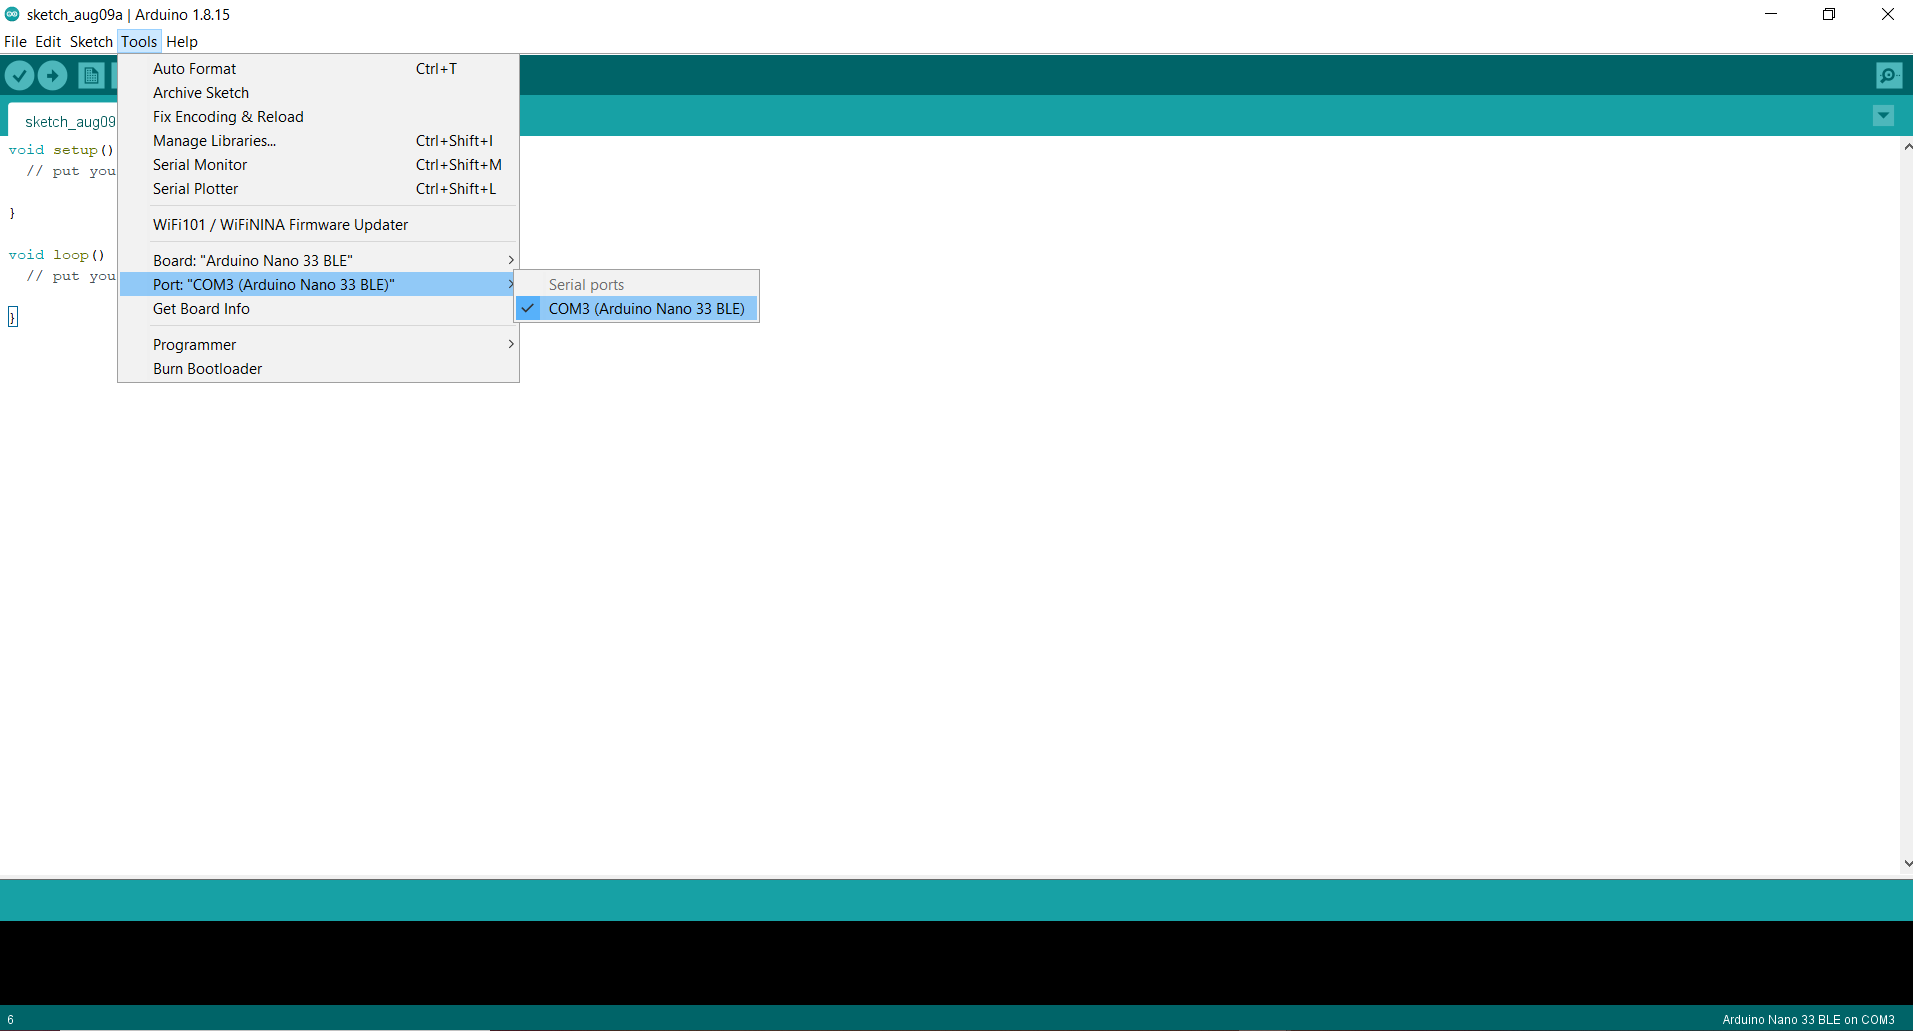
\includegraphics[width=1.0\linewidth]{Nano33BLESense/Port-Select}
	\caption{Select Available Port for Uploading Arduino Sketch}
	\label{fig:Port-Selection}
\end{figure}

\subsection{Upload Code in Arduino Board}

By making sure to select the appropriate port, it's time to upload the Arduino program. There are five icons (verify, upload, new, open, save) below the file section, before uploading the program the best practice is to verify the program first, it show us if there are any error or warning in the program exist or not. By successfully verifying the program we can safely upload the program by click the upload button in the top below the file section as shown in figure. \ref{fig:Upload}.


\begin{figure}[h]
	\centering
	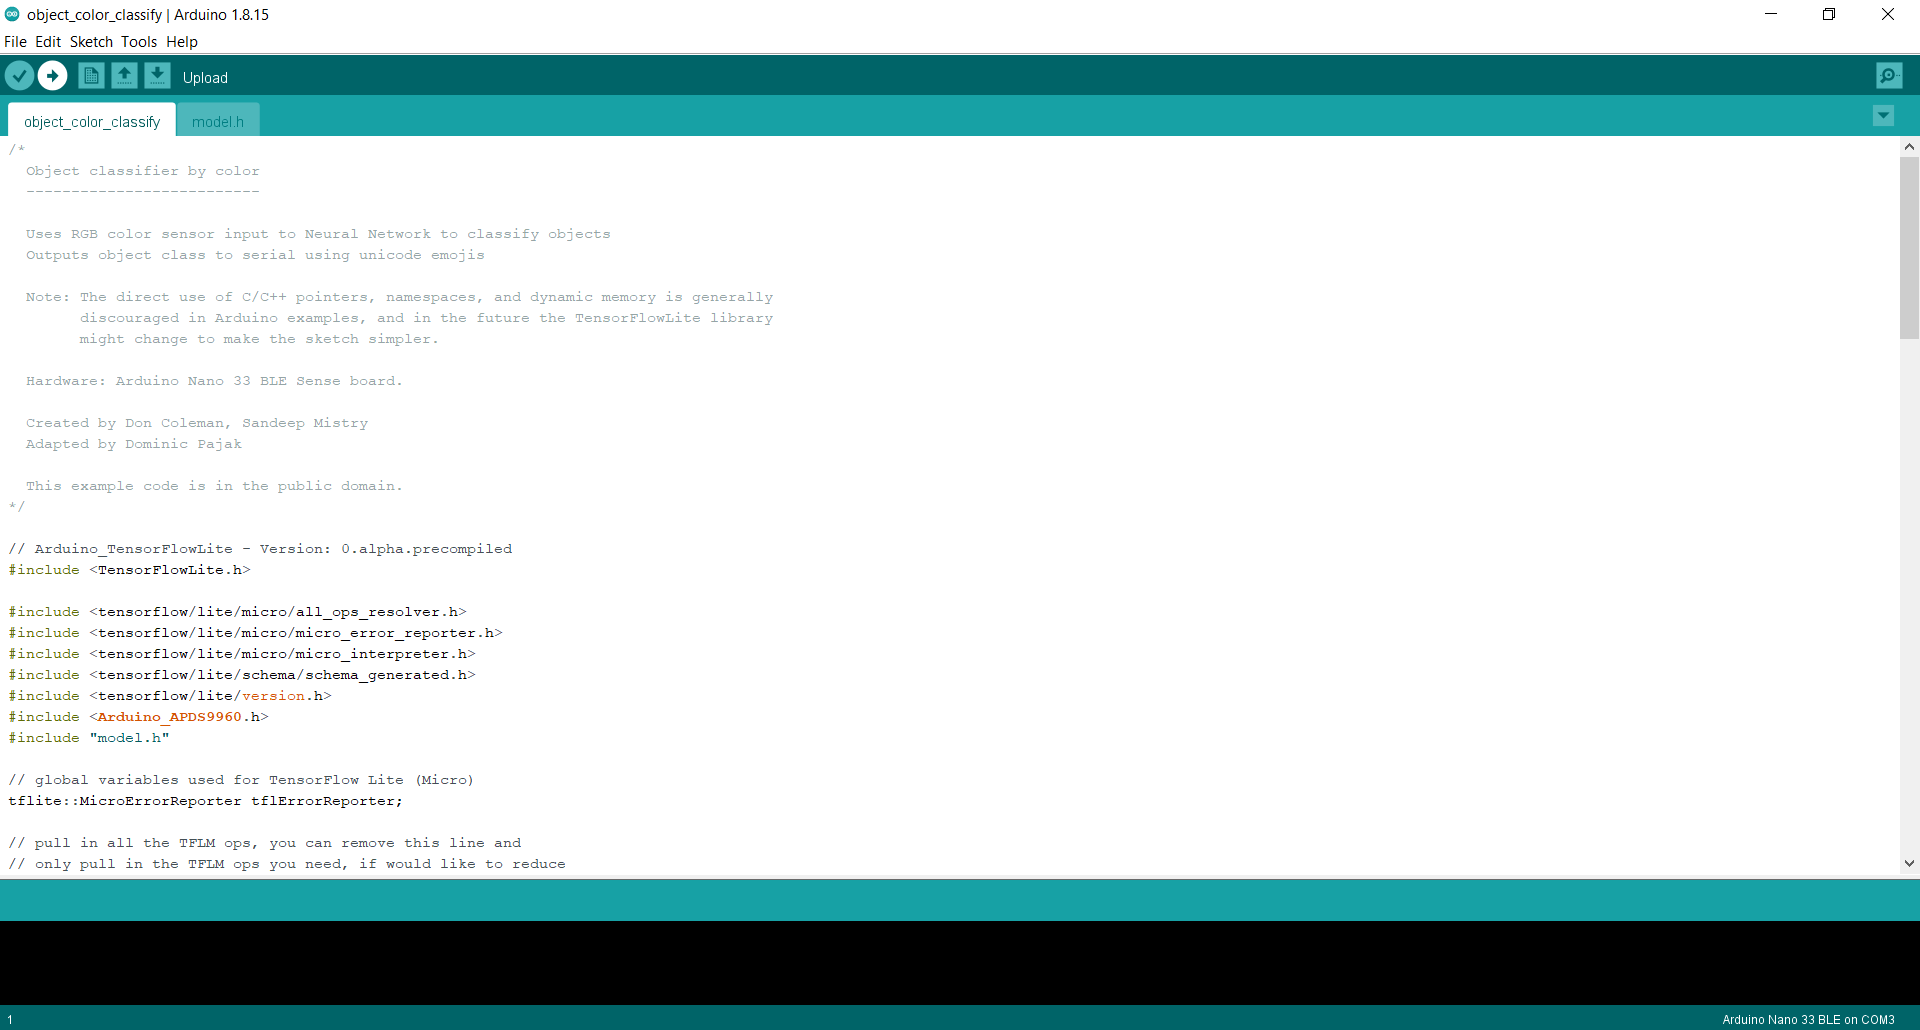
\includegraphics[width=1.0\linewidth]{Nano33BLESense/Upload}
	\caption{Upload the Program in Arduino board}
	\label{fig:Upload}
\end{figure}

After uploading, the code will compile and if there is any issue in our program it will pop up in the bottom black window as well.

After successfully uploading and compiling the code in Arduino board, it also require to change the port again as we did it previously. Go to tool select arduino port and make sure to check the port again as shown in figure \ref{fig:Port} by getting output in the serial monitor.

\begin{figure}[h]
	\centering
	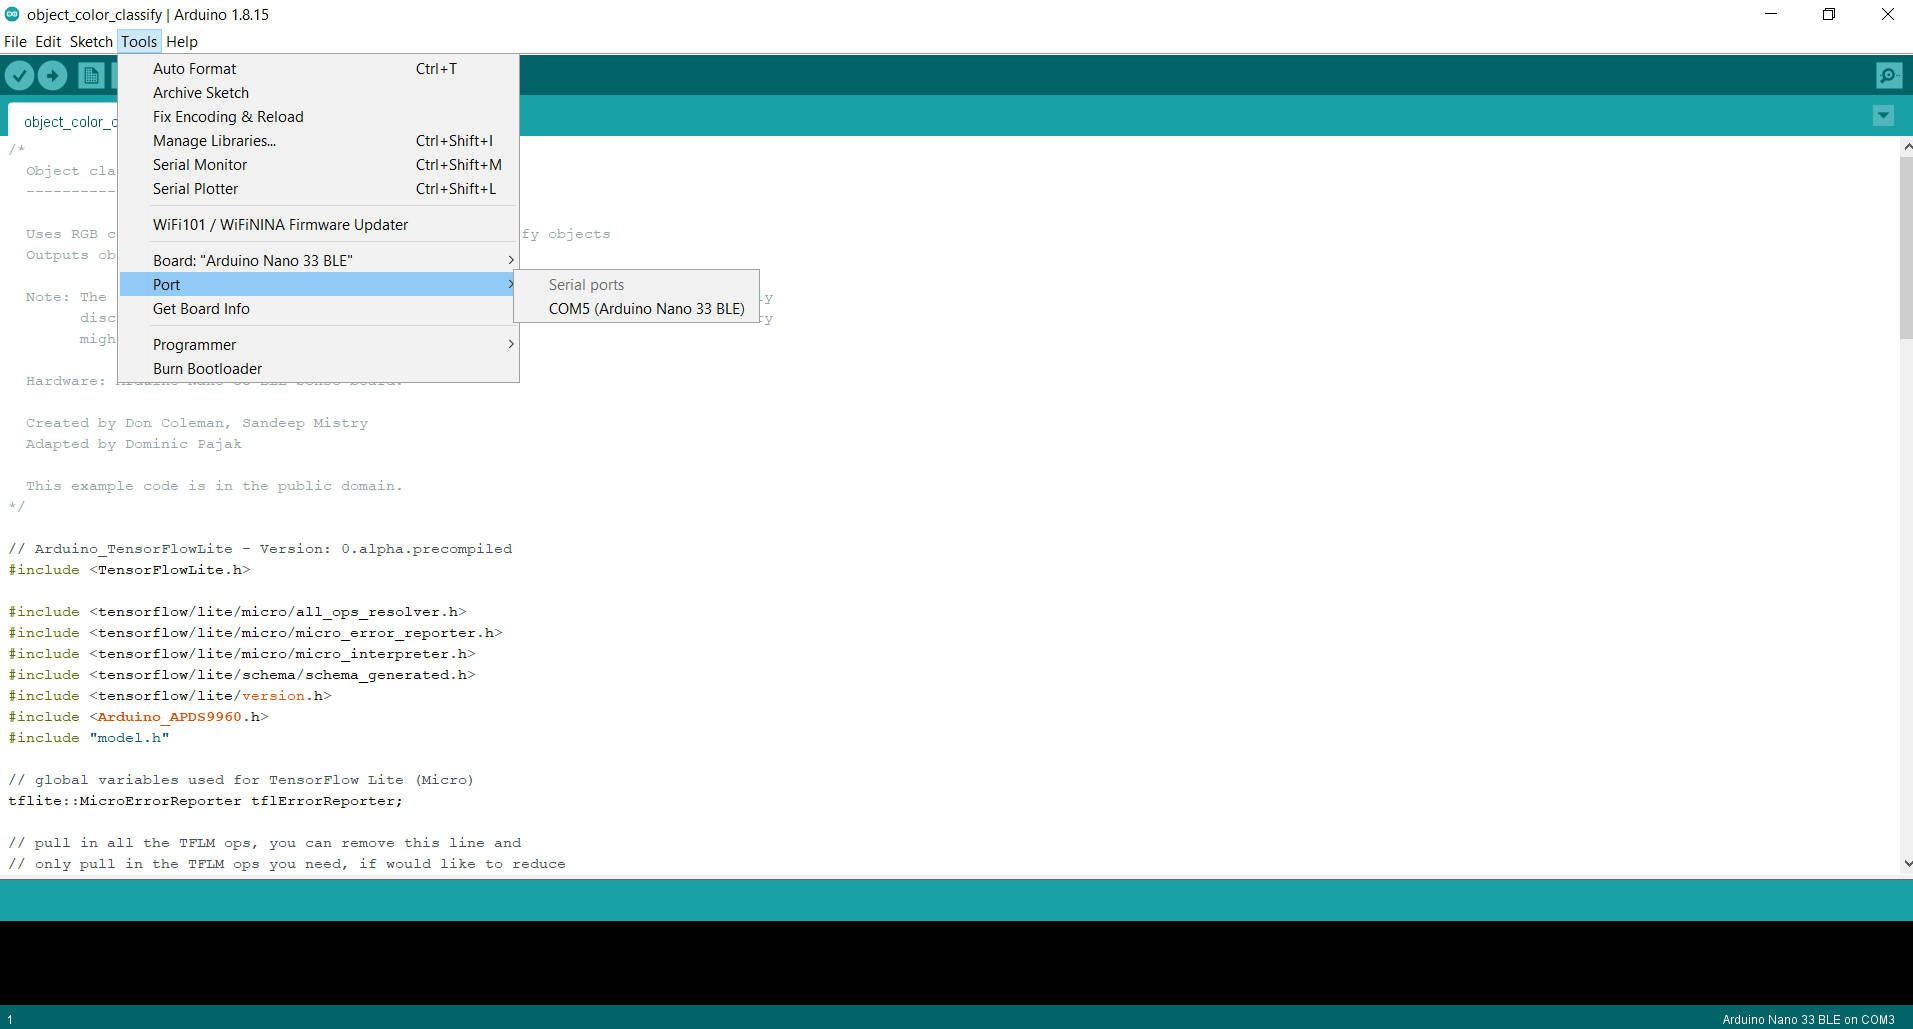
\includegraphics[width=1.0\linewidth]{Nano33BLESense/Port}
	\caption{Setting the Port}
	\label{fig:Port}
\end{figure}

\section{Output Window (Serial Monitor)}

Serial Monitor is the another window on the Arduino IDE, which shows the Input/Output of our program and results appear on it as per the required output. For getting access to Serial monitor, we need to go extreme right in the Arduino IDE, the small circle pop up when we reach it is the serial monitor as show in the figure. \ref{fig:Serial Monitor}

\begin{figure}[h]
	\centering
	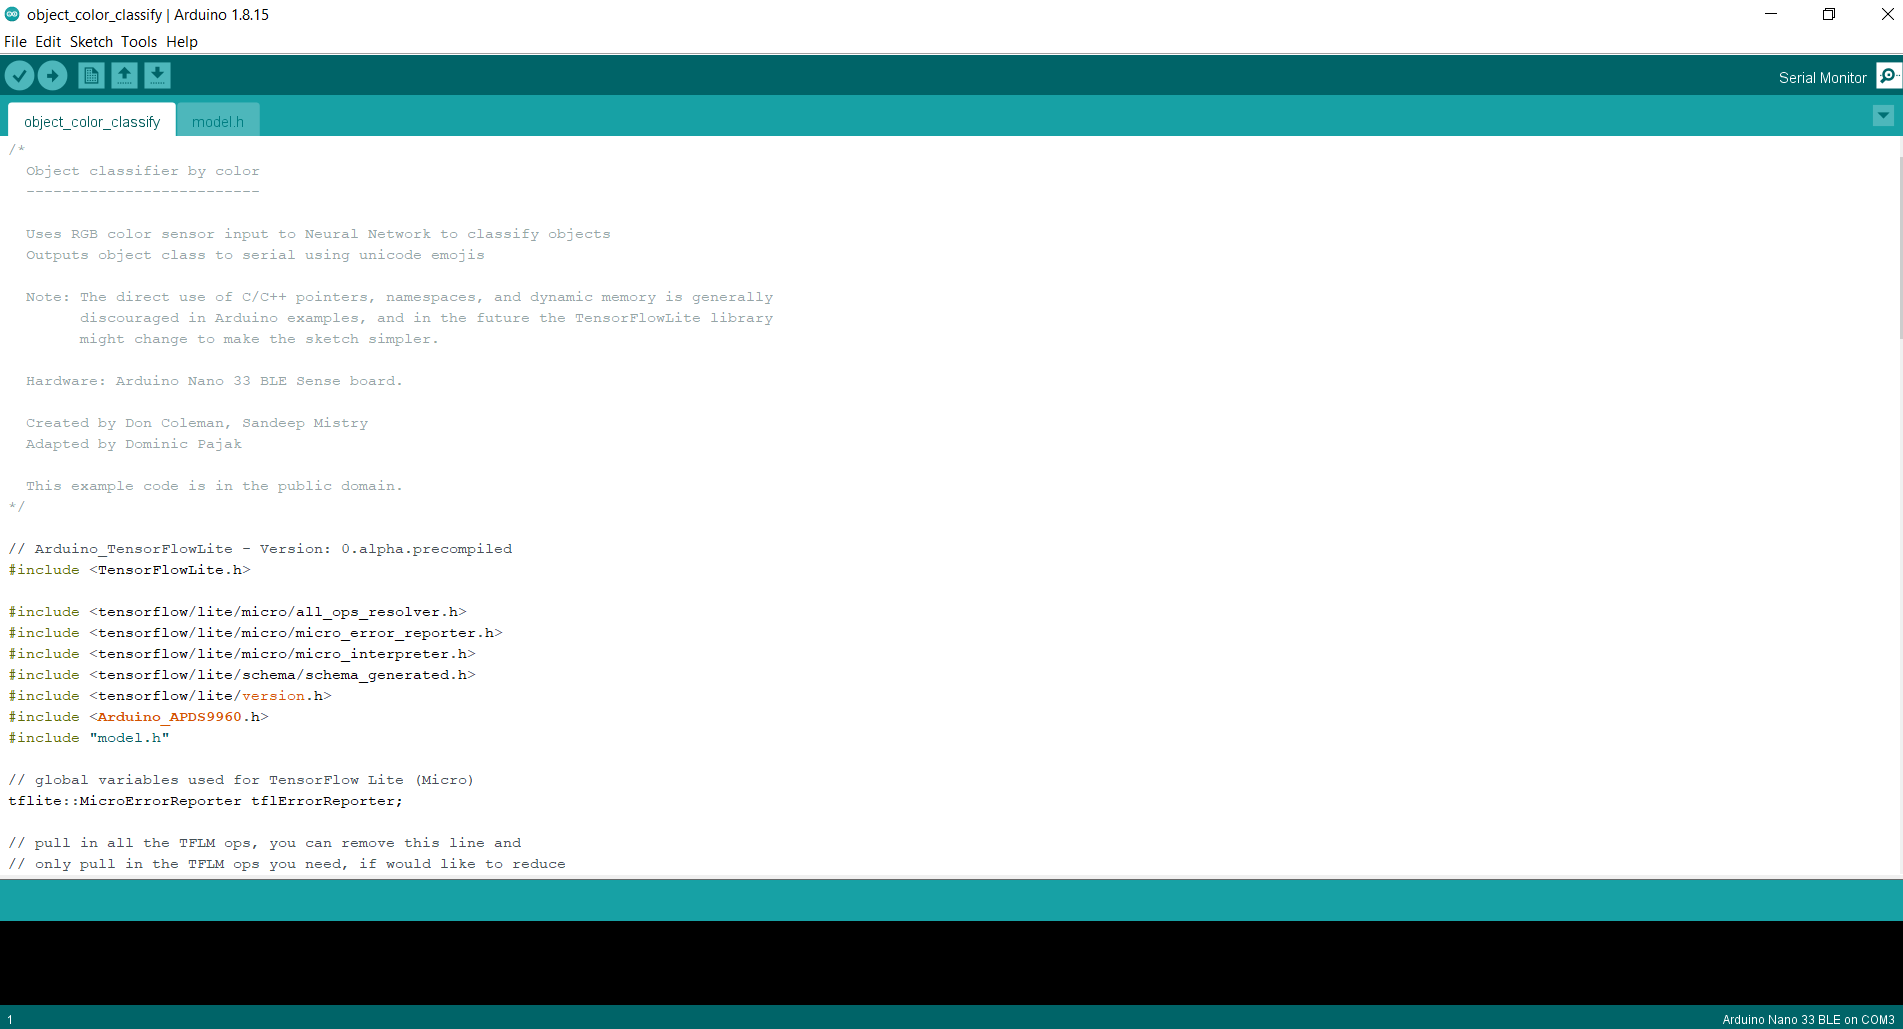
\includegraphics[width=1.0\linewidth]{Nano33BLESense/Serial Monitor}
	\caption{Serial Monitor Icon}
	\label{fig:Serial Monitor}
\end{figure}

The Final results, all the variables, input, sensor values are shown in the serial monitor the (Output Window)  as shown in the figure \ref{fig:Output Window} by clicking the serial monitor button.

\begin{figure}[h]
	\centering
	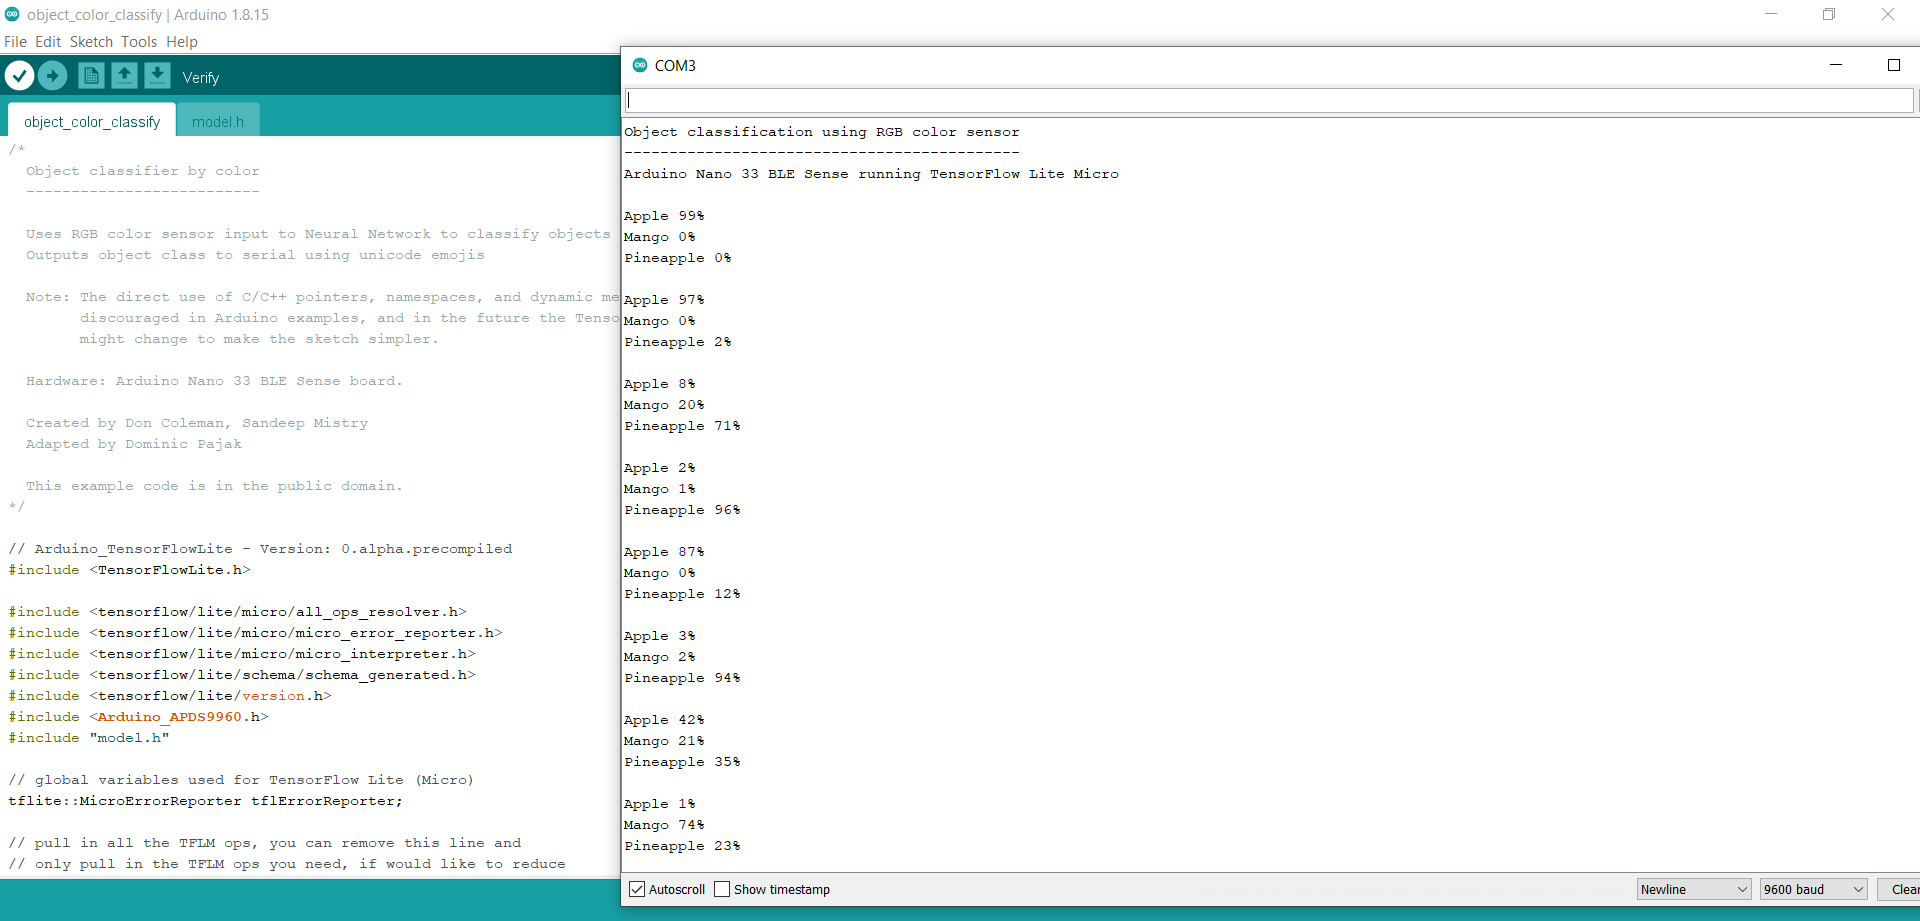
\includegraphics[width=1.0\linewidth]{Nano33BLESense/4}
	\caption{Output Window}
	\label{fig:Output Window}
\end{figure}

\section{Python on Pycharm}

PyCharm is an integrated development environment (IDE) from the JetBrains company for the Python programming language. This Integrated development environment offers only the python programming environment, which will be usefull later in our project for running some computer vision python module.


\subsection{Pycharm Installation}

For getting up to date latest version of pycharm, we need to go \href{https://www.jetbrains.com/pycharm/download/#section=windows}{JetBrains-Link} and install the appropriate version as per our Operating system. 

\section{Python Installation}

Python is commonly used for developing websites and software, task automation, data analysis, and data visualization. Since it's relatively easy to learn, Python has been adopted by many non-programmers such as accountants and Data scientists, for a variety of everyday tasks, like organizing finances. It is an interpreted, object-oriented, high-level programming language with dynamic semantics. \href{https://www.python.org/downloads/}{Python Installation} at the time of writing this report the latest version of python is 3.9.7 release.\ref{Python Installation}

\begin{figure}[h]
	\centering
	\includegraphics[width=1.0\linewidth]{Nano33BLESense/python}
	\caption{Python Installation}
	\label{Python Installation}
\end{figure}

\section{Anaconda supporting framework for Jupyter Notebook}

Anaconda is a distribution of the Python and R programming languages for scientific computing (data science, machine learning applications, large-scale data processing, predictive analytics, etc.), that aims to simplify package management and deployment. It is the most popular toolkit for data science environment. It support every package of Machine learning and Artificial Intelligence. The most widely used packages in machine learning are TensorFlow, OpenCV, and MediaPipe. the other supporting libraries include Numpy, Pandas, Matplotlib, Sklearn and many more. For getting up to date documentation and installation guide available at \href{https://www.anaconda.com/products/individual}{Jupyter notebook}. Anaconda support Jupyter notebook web application, it is the most widely used notebook for writing and training the Machine learning models.


\chapter{Test}

\section{General Tests}

All the Arduino boards need power to operate, either it comes from the USB connection with Laptop, Ac power adapter, Battery or a regulated power supply. The most easiest way to operate arduino board is USB connection with laptop, normally these boards need 5V direct current (DC) to operate. Arduino Nano 33 BLE sense also need these types of power sources for funcnality, when applying one of the above mention power source the green LED glows as shown in the figure \ref{fig:Test}, it shows the sign of Arduino board working.

\begin{figure}[htbp]
	\centering
	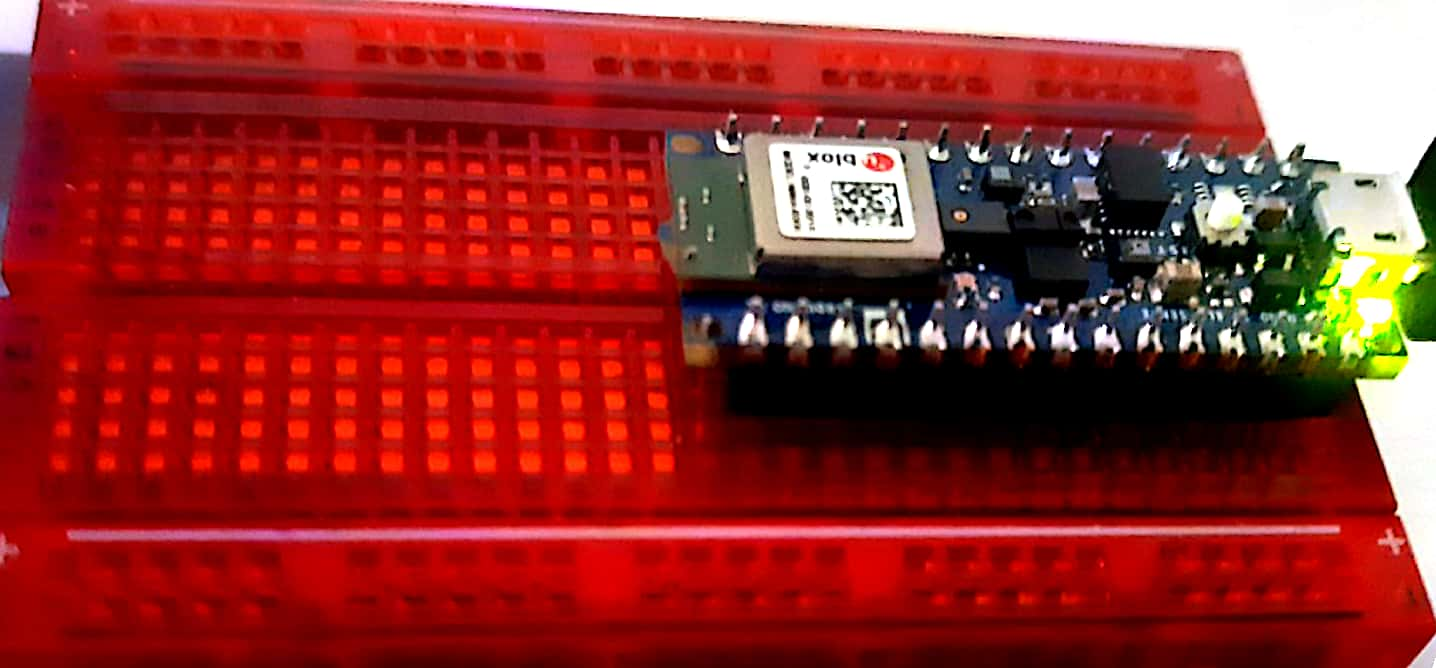
\includegraphics[width=6.5cm]{Nano33BLESense/Test-1}
	\caption{Power On Arduino Nano 33 BLE Sense}
	\label{fig:Test}
\end{figure}

\section{Testing the On-Board Sensor}

Arduino Nano 33 BLE sense have a set of on-board sensor embed on it. These sensor also start working when arduino board operate. These are the following set of sensors available in Arduino Nano 33 BLE Sense board.
\begin{itemize}
	\item The IMU is a LSM9DS1 and it is managed through I2C.
	\item The LPS22HB reads barometric pressure and environmental temperature.
	\item The HTS221 senses relative humidity.
	\item The ADPS-9960 is a digital proximity, ambient light, RGB and gesture sensor.
	\item The MP34DT05 is the digital microphone.
\end{itemize} 

\subsection{LSM9DS1 (Accelerometer, Gyroscope, and Magnetometre Sensor)}

The 9-axis inertial measurement unit (IMU) sensor is work as a accelerometre, gyroscope, and magnetic sensor. It measures 3D linear acceleration, 3D angular Velocity and 3D magnetic field aroud the sensor. This 9-axis IMU sensor use to measure Position, vibration, orientation and magnetic field around the sensor. To check the funcnality of this sensor there is avialable library in the example section as shown in the figure. \ref{fig:Testware} Go to examples check LSM9DS1 sensor, it shows all the functionality of this sensor i.e: (Accelerometer, Gyroscope, and Magnetometer).


\begin{figure}[htbp]
	\centering
	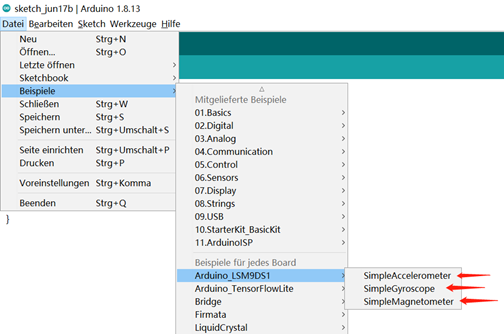
\includegraphics[width=7.5cm]{Nano33BLESense/Testware3Sensoren}
	\caption{9-Axis IMU Sensor}
	\label{fig:Testware}
\end{figure}

By getting the results and output of the 9-axis IMU sensor, first we need to upload the available library program into Arduino nano 33 BLE Sense. To avoid any trouble during uploading the program, make sure to follow all the steps as we discussed in previous chapter e.g; (choose the board, select the port during upload and change the port when need to see output in serial monitor, reset arduino when needed). By uploading the program successfully, open the serial monitor and see the result as shown in figure.\ref{fig:IMU-Test} Make sure to change the position and orientation of board and also place some Magnet aroud the borad, it shows visible changes in the output too.

\begin{figure}[htbp]
	\centering
	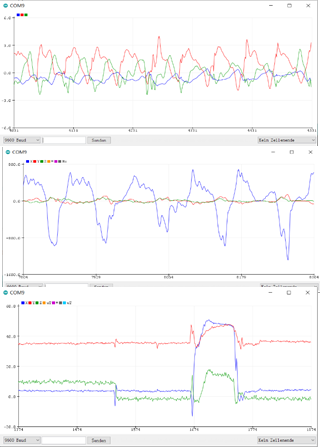
\includegraphics[width=7.5cm]{Nano33BLESense/ErgebnisseIMUTests}
	\caption{Results of IMU-Tests}
	\label{fig:IMU-Test}
\end{figure}

The above 9-Axis IMU output, shows the 3-axis values for each accelerometer, gyroscope and magnetometer. It shows how powerful the Arduino Nano 33 ble sense board and compatible with Arduino IDE the integrated development environment. These values changes as the sensor observes some changing in the sorroundings too, and it shows in the form of graph in the serial monitor. 


\subsection{APDS-9960 (Gesture, Proximity, and Color Detection Sensor)}
APDS-9960 sensor has the funcnality of proximity distance measure, RGB color detection, and Gesture detection too. It is also on-board embed sensor on Arduino nano 33 BLE Sense and has the same procedure for uploading and compiling the program as the 9-axis IMU sensor has. Go to example, check the APDS-9960 library and upload the complete program as shown in the figure. \ref{fig:1} Full example includes the RGB color detection code, gesture detection code, and also proximity distance measure code.

\begin{figure}[htbp]
	\centering
	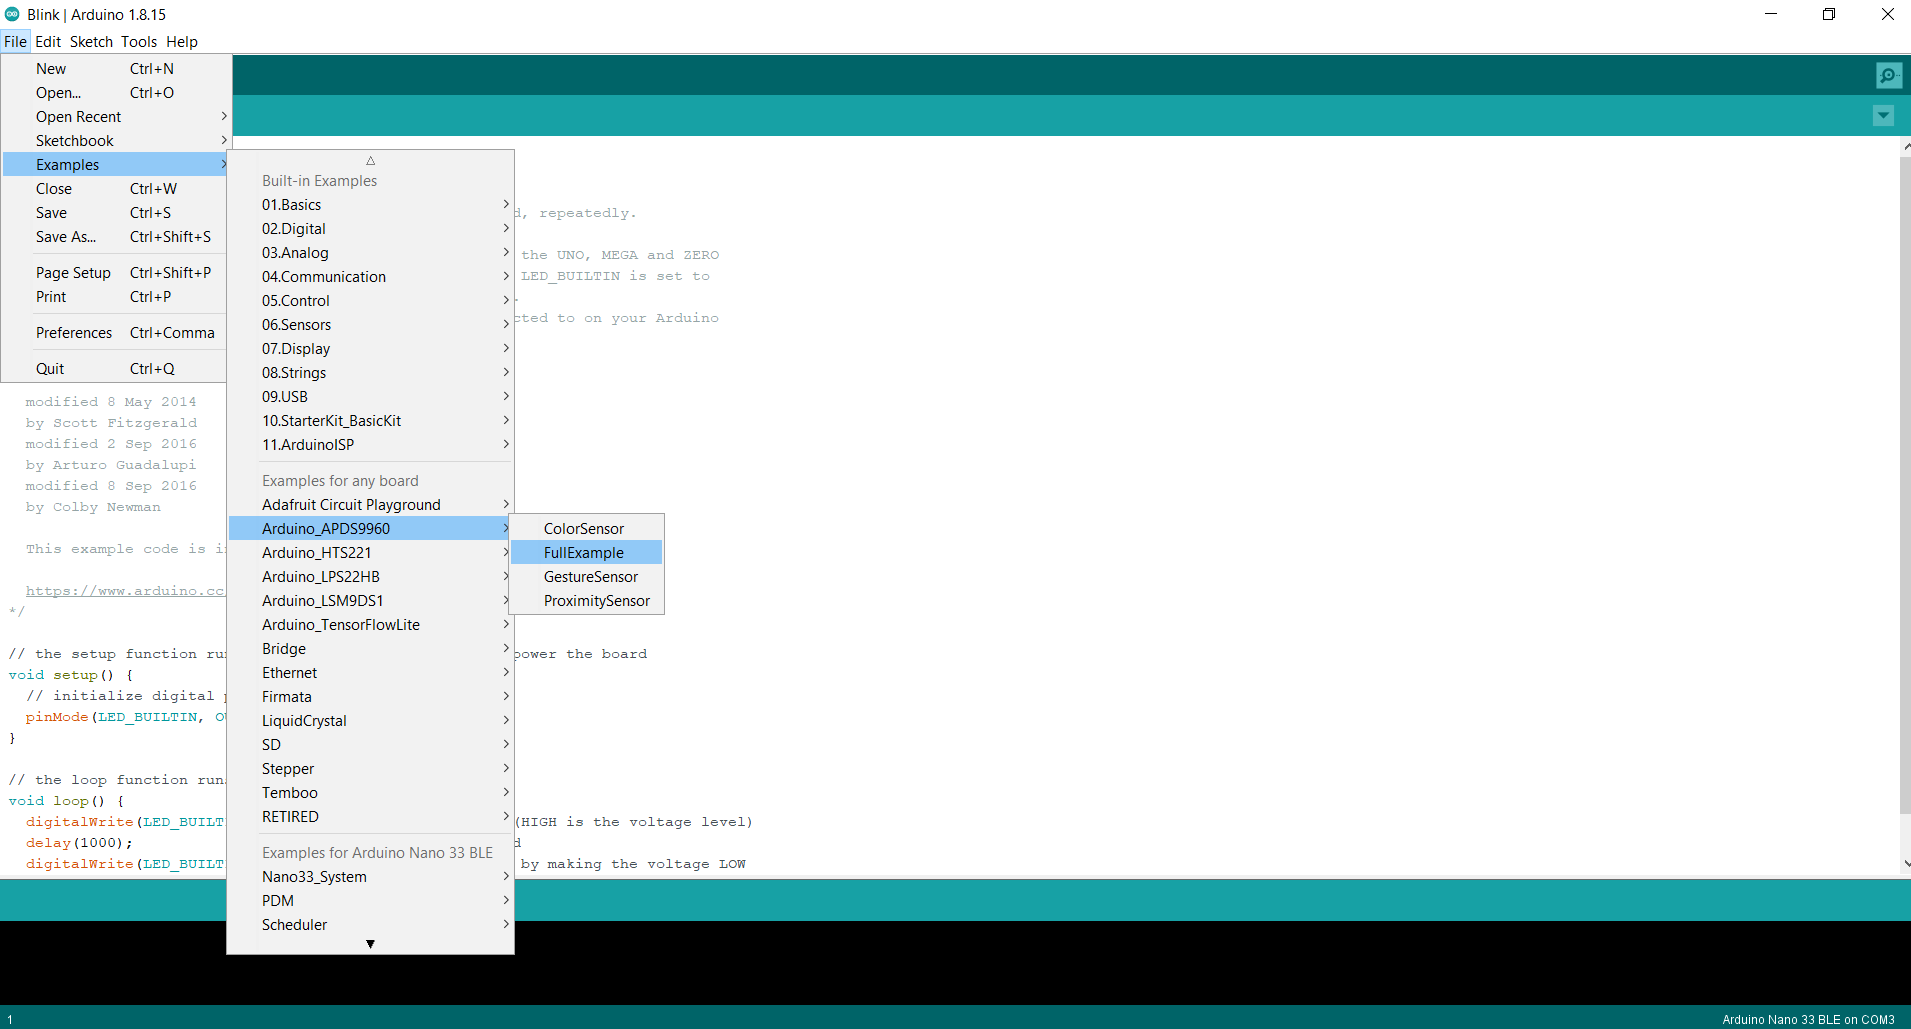
\includegraphics[width=7.5cm]{Nano33BLESense/APDS}
	\caption{APDS-9960 Gesture, Proximity, Color Sensor}
	\label{fig:1}
\end{figure}

Similarly, by following all the steps for uploading and compiling the program we can see the results of APDS-9960 Sensor on serial monitor too. For seeing the different output, we can change the input for the sensor too, e.g: for color detection we can switch the colors, for gesture detection we can also switch the gestures, and for proximity also do the same. The resulted output as shown in the figure.  \ref{fig:2} 

\begin{figure}[htbp]
	\centering
	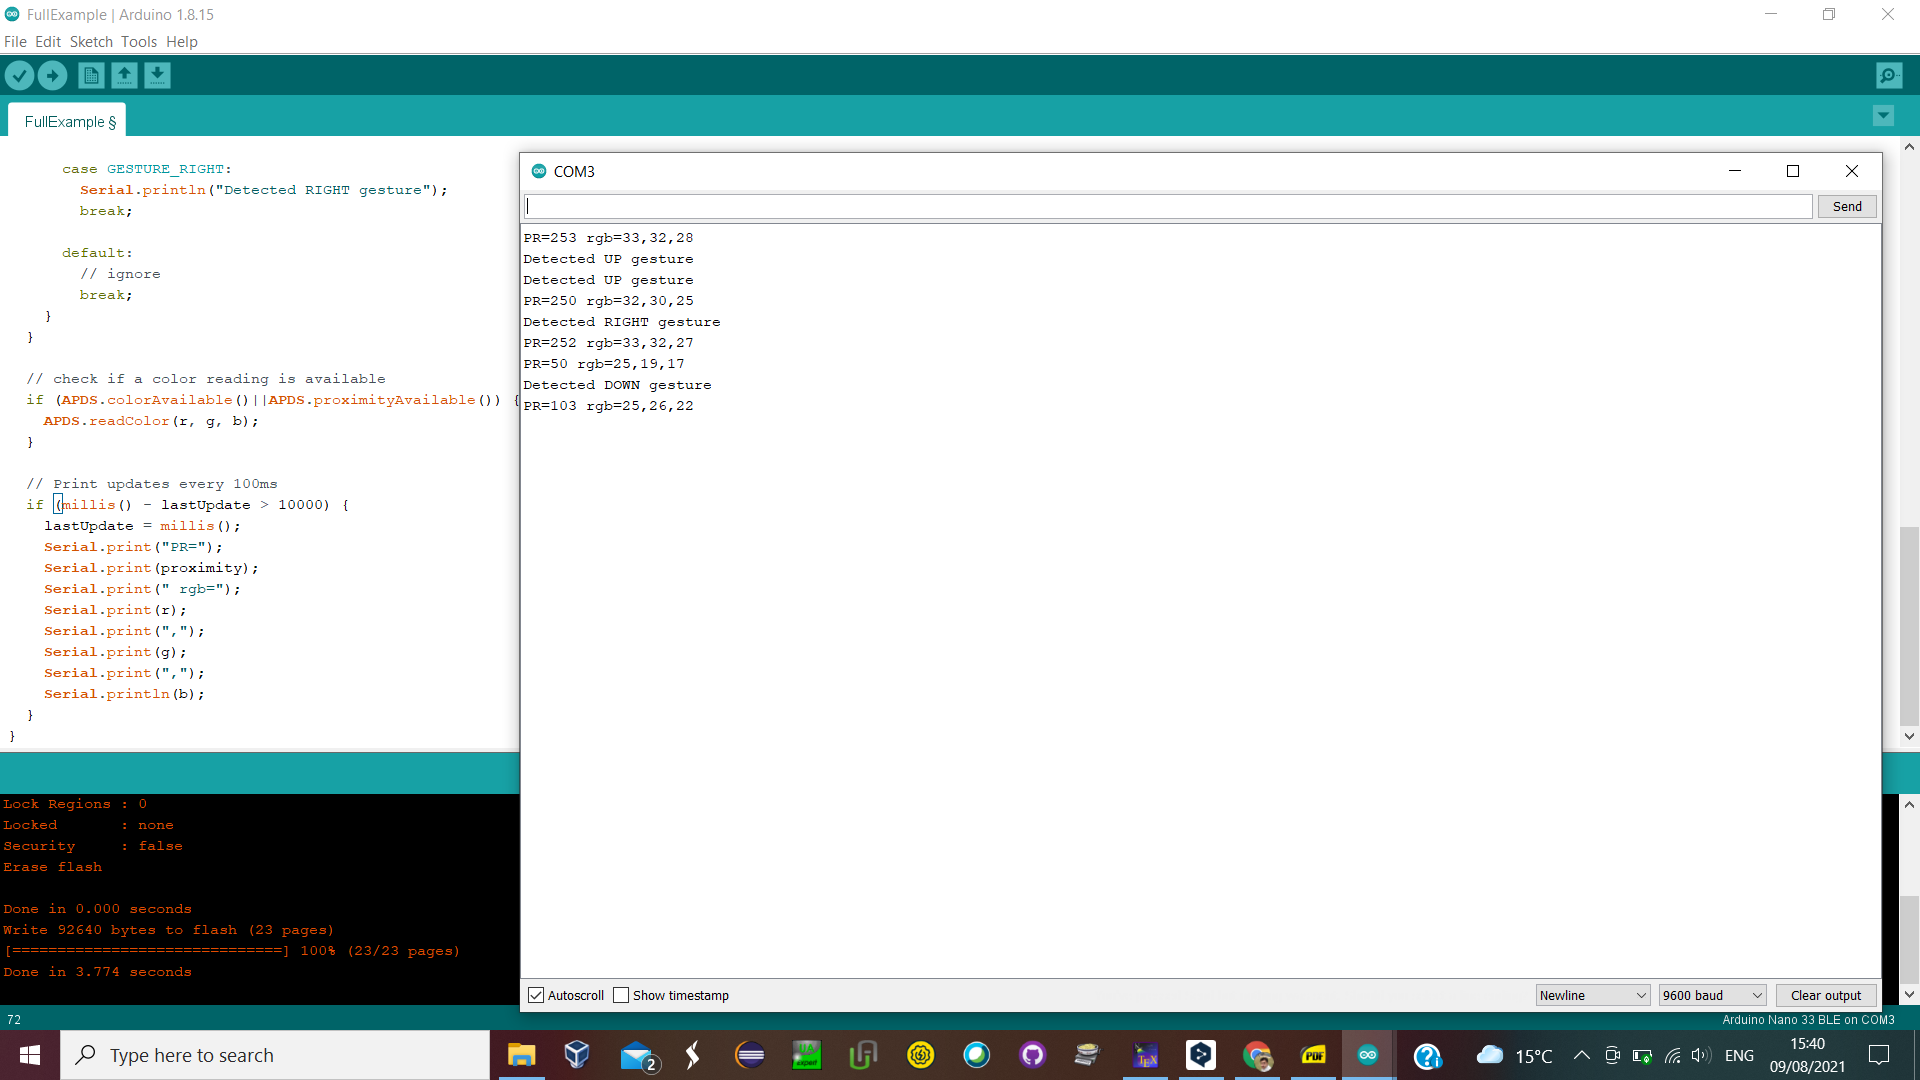
\includegraphics[width=9.5cm]{Nano33BLESense/APDS-Output}
	\caption{Gesture, Proximity, Color Sensor Output Window}
	\label{fig:2}
\end{figure}

We can also run the single funcnality of this sensor too, e.g; if we just need to capture the color of product, we can also run the color detection program. It depends upon the application and we can implement our application and modify the code as per our desire results.

\subsection{LPS22HB (Pressure Sensor)}
Arduino Nano 33 BLE sense also capable of measuring environmental or ambient pressure with the help of LPS22HB on-board embed sensor on it. There is also available library program in Arduino IDE, we need to install the appropriate library and use it or  modify it as per the required application. The procedure for uploading and compiling the code is same as the above sensors have. By opening the example section from file, then go to LPS22HB and click on read or measuring pressure as shown in the figure.  \ref{fig:3} 

\begin{figure}[htbp]
	\centering
	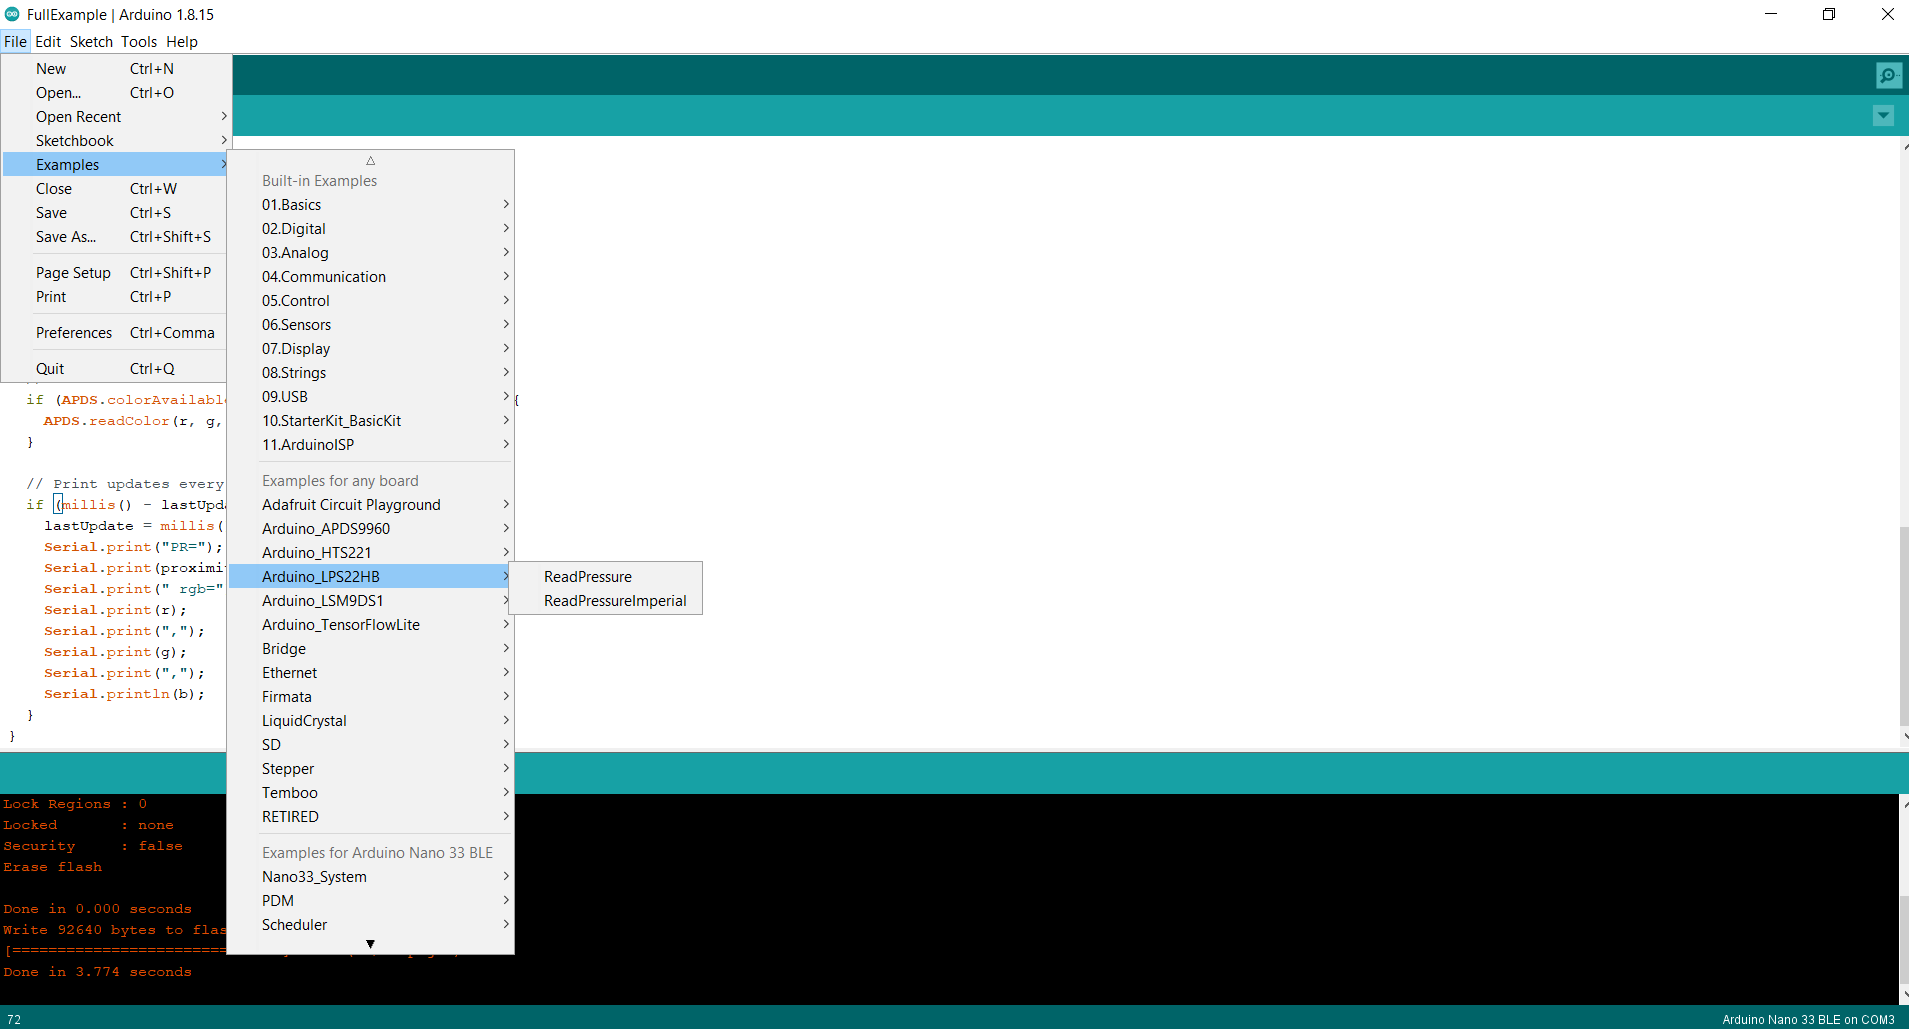
\includegraphics[width=8.5cm]{Nano33BLESense/5}
	\caption{LPS22HB, Pressure and Temperature sensor}
	\label{fig:3}
\end{figure}

The results for LPS22HB the environmental pressure also showed in the serial monitor as shown in the figure.  \ref{fig:4} With the help of these values and modifying the code we can operate some external devices or also just measure the external or internal pressure and apply it wherever it needs.

\begin{figure}[htbp]
	\centering
	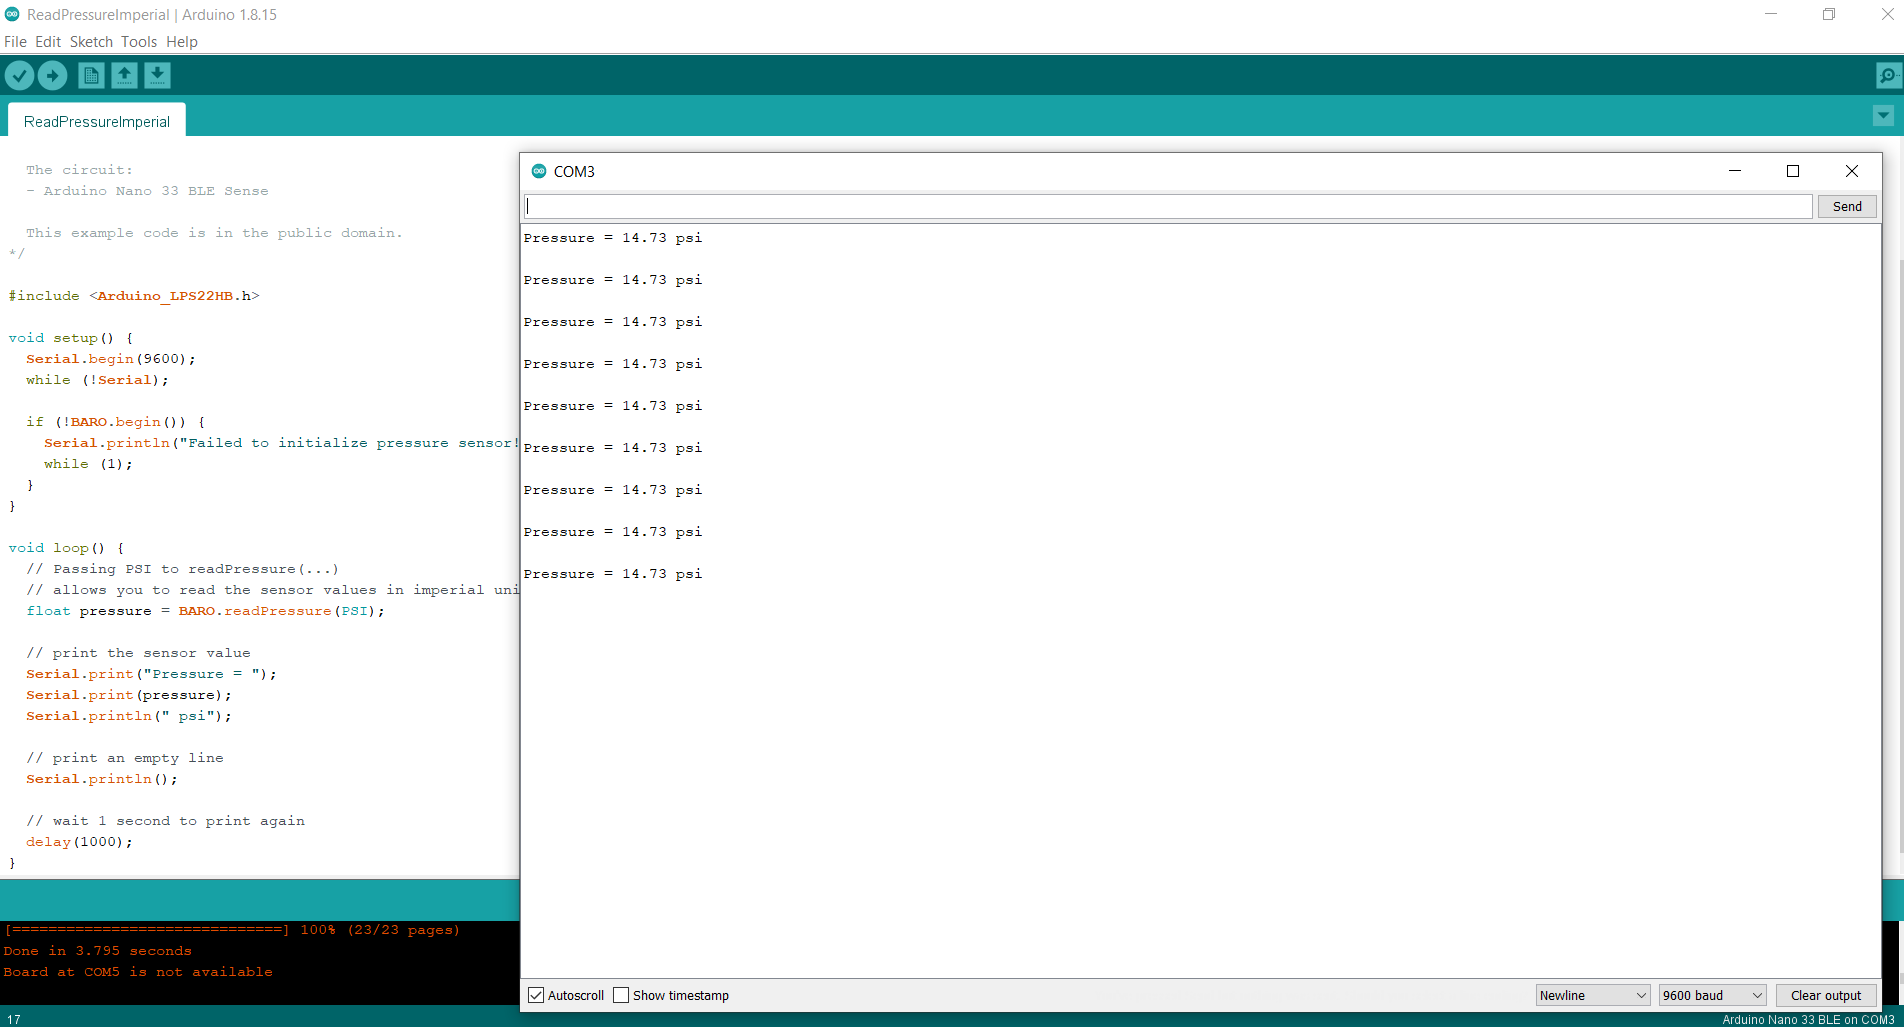
\includegraphics[width=8.5cm]{Nano33BLESense/6}
	\caption{LPS22HB, Output}
	\label{fig:4}
\end{figure}

\subsection{HTS221 (Humidity and Temperature Sensor)}

\begin{figure}[htbp]
	\centering
	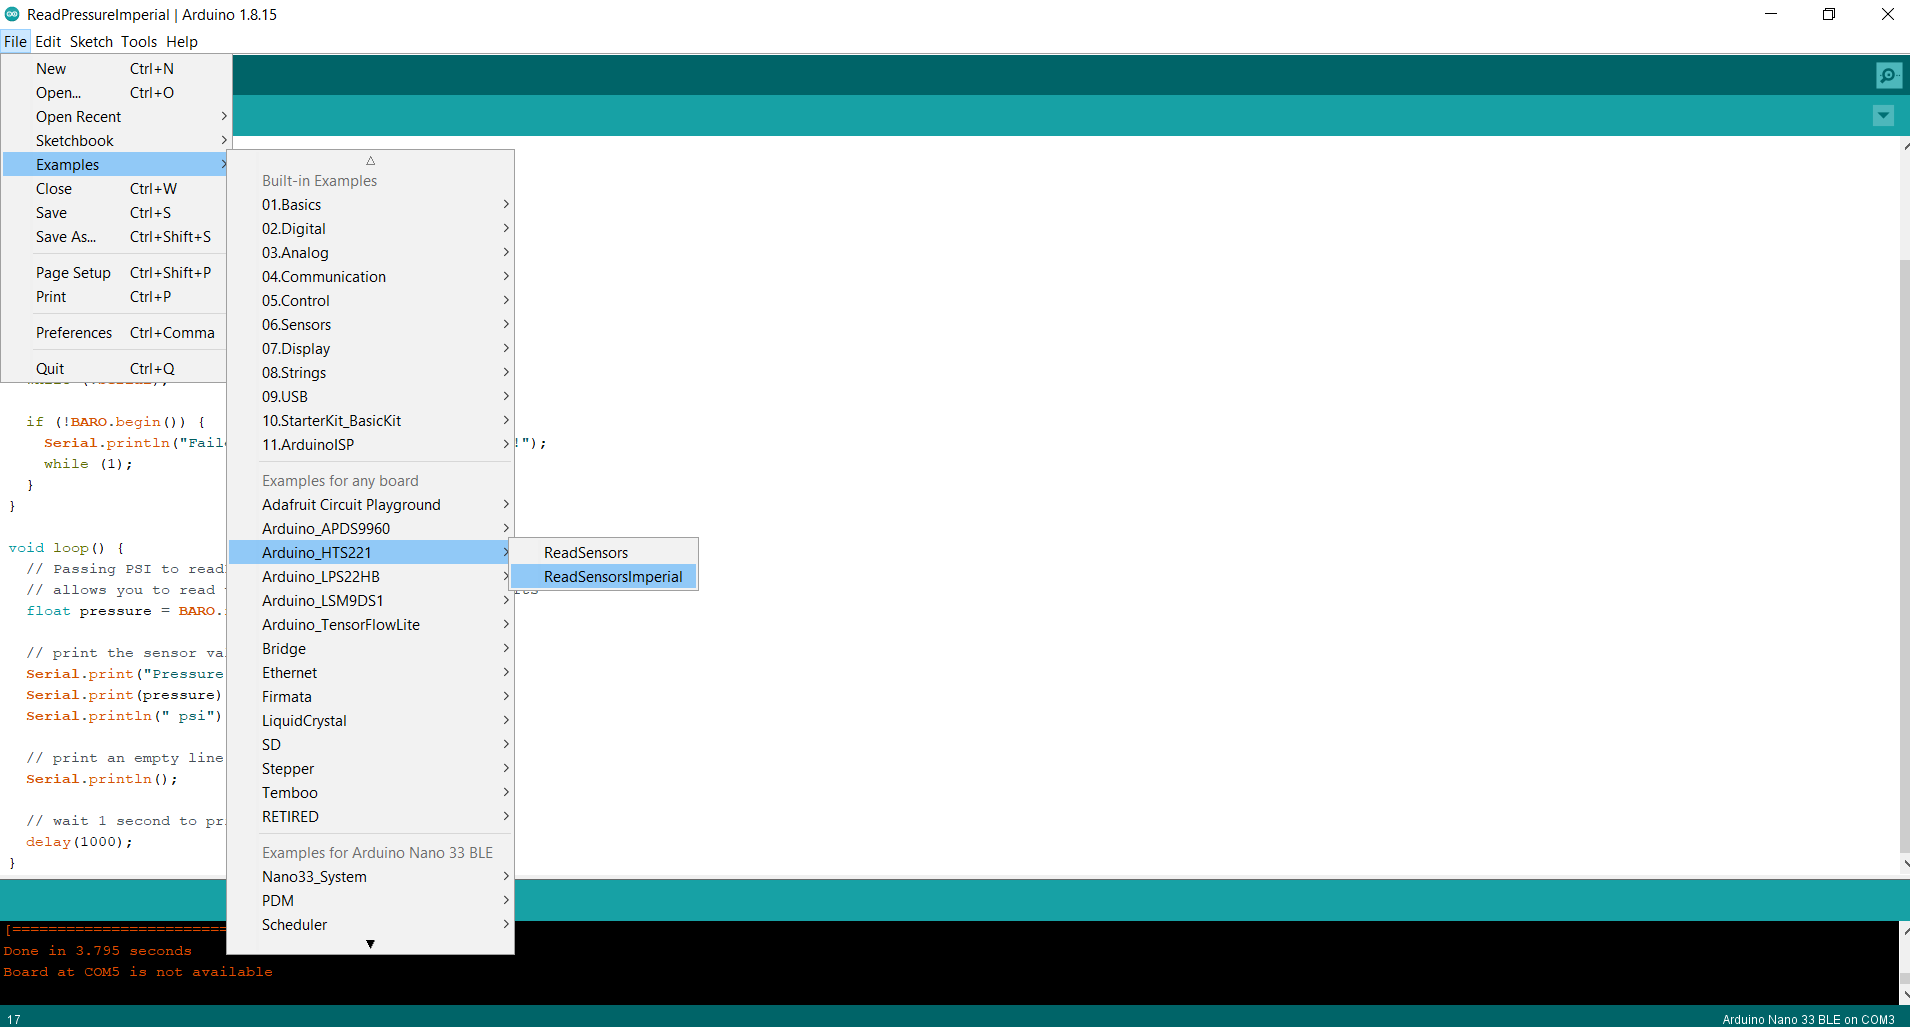
\includegraphics[width=8cm]{Nano33BLESense/7}
	\caption{HTS221, Humidity and Temperature Sensor}
	\label{fig:5}
\end{figure}

The on-board embed HTS221 sensor on Arduino Nano 33 BLE Sense has the funcnality to measure the relative humadity and temperature in the environment. The procedure for getting access to his library and code also the same as the other sensors have as shown in the figure.  \ref{fig:5}

After Uploading and compiling the program, the environmental humidity and temperature also display in the serial monitor as shown in the figure.  \ref{fig:6} By getting access to these values, change the port again after compiling the program for opening the serial monitor, these values help us to make the application with electrical appliances regarding energy savings or modify the code and add some external devices with the GPIO of Arduino Nano 33 BLE Sense too and control it as per the humidity and temperature values.

\begin{figure}[htbp]
	\centering
	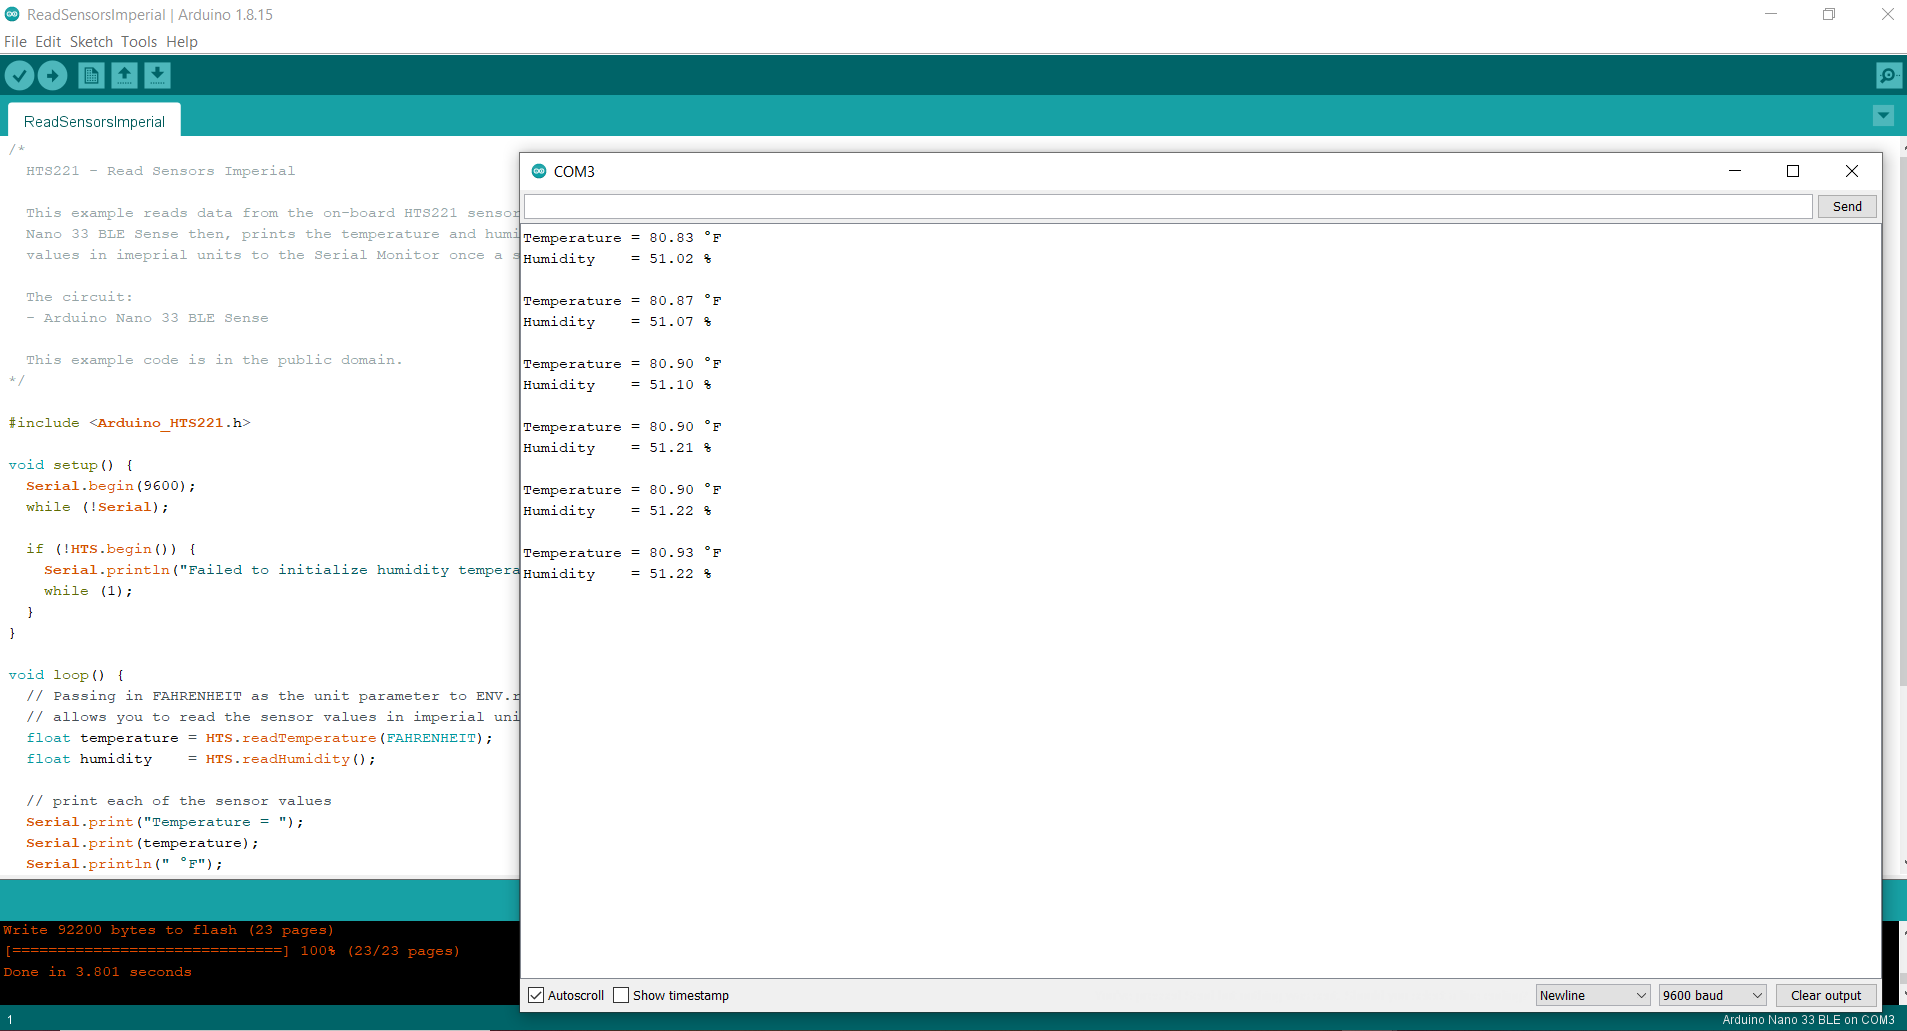
\includegraphics[width=8.5cm]{Nano33BLESense/8}
	\caption{HTS221, Output Window}
	\label{fig:6}
\end{figure}

\subsection{MP34DT05 (Digital Microphone)}

The embed on-board MP34DT05 sensor in Arduino Nano 33 BLE Sense has the funcnality to sense audio voice from the environment. There is build in Arduino library for this particular sensor, which is PDM as shown in the figure.  \ref{fig:7}

\begin{figure}[htbp]
	\centering
	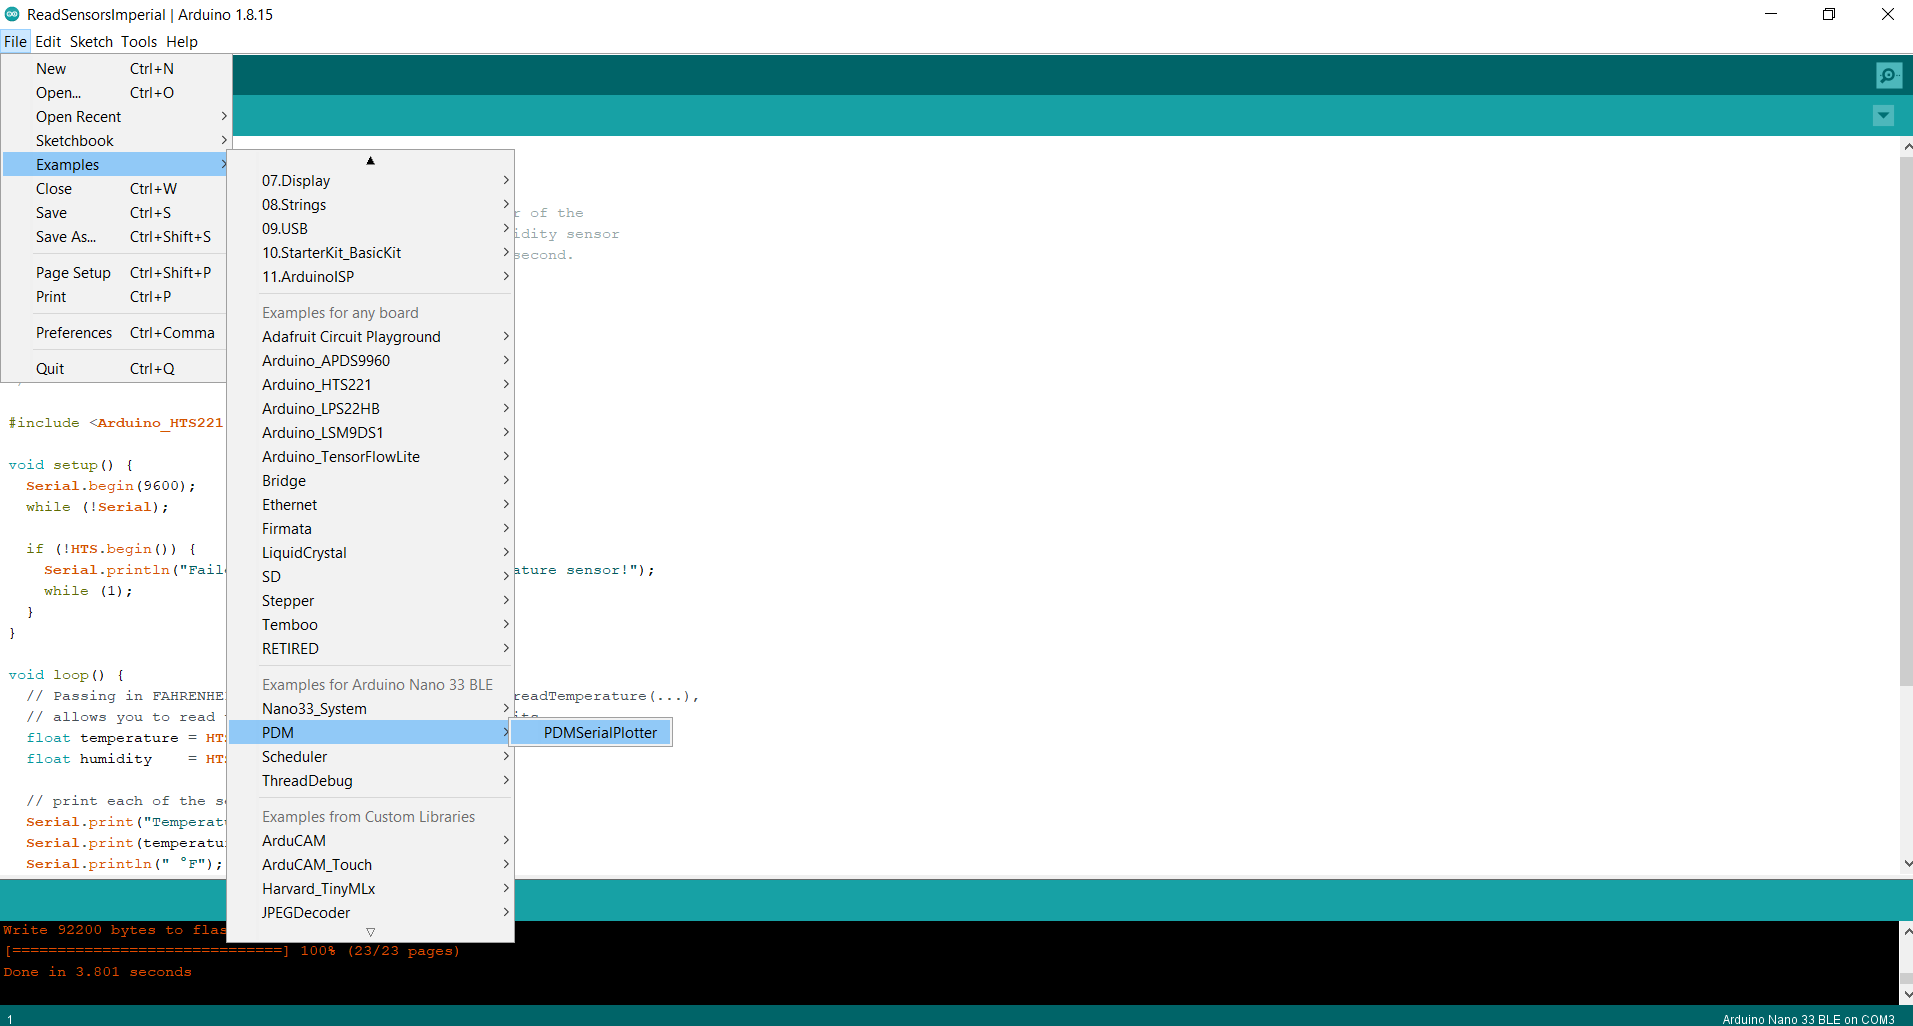
\includegraphics[width=8.5cm]{Nano33BLESense/9}
	\caption{MP34DT05, Digital Microphone}
	\label{fig:7}
\end{figure}

By following the same steps, for this sensor we can see the output the resulted frequency in the serial plotter instaed of serial monitor as shown in figure.  \ref{fig:8}  It is more convenient to understand if we change the loudness of voice the plotter shows us a different frequency curve. MP34DT05 use to detect different voices or words too, with the help of these funcnality we can easily make the valuable application with Arduino Nano 33 BLE Sense by adding some external devices with GPIO pins with the help of 3.3V relay.

\begin{figure}[htbp]
	\centering
	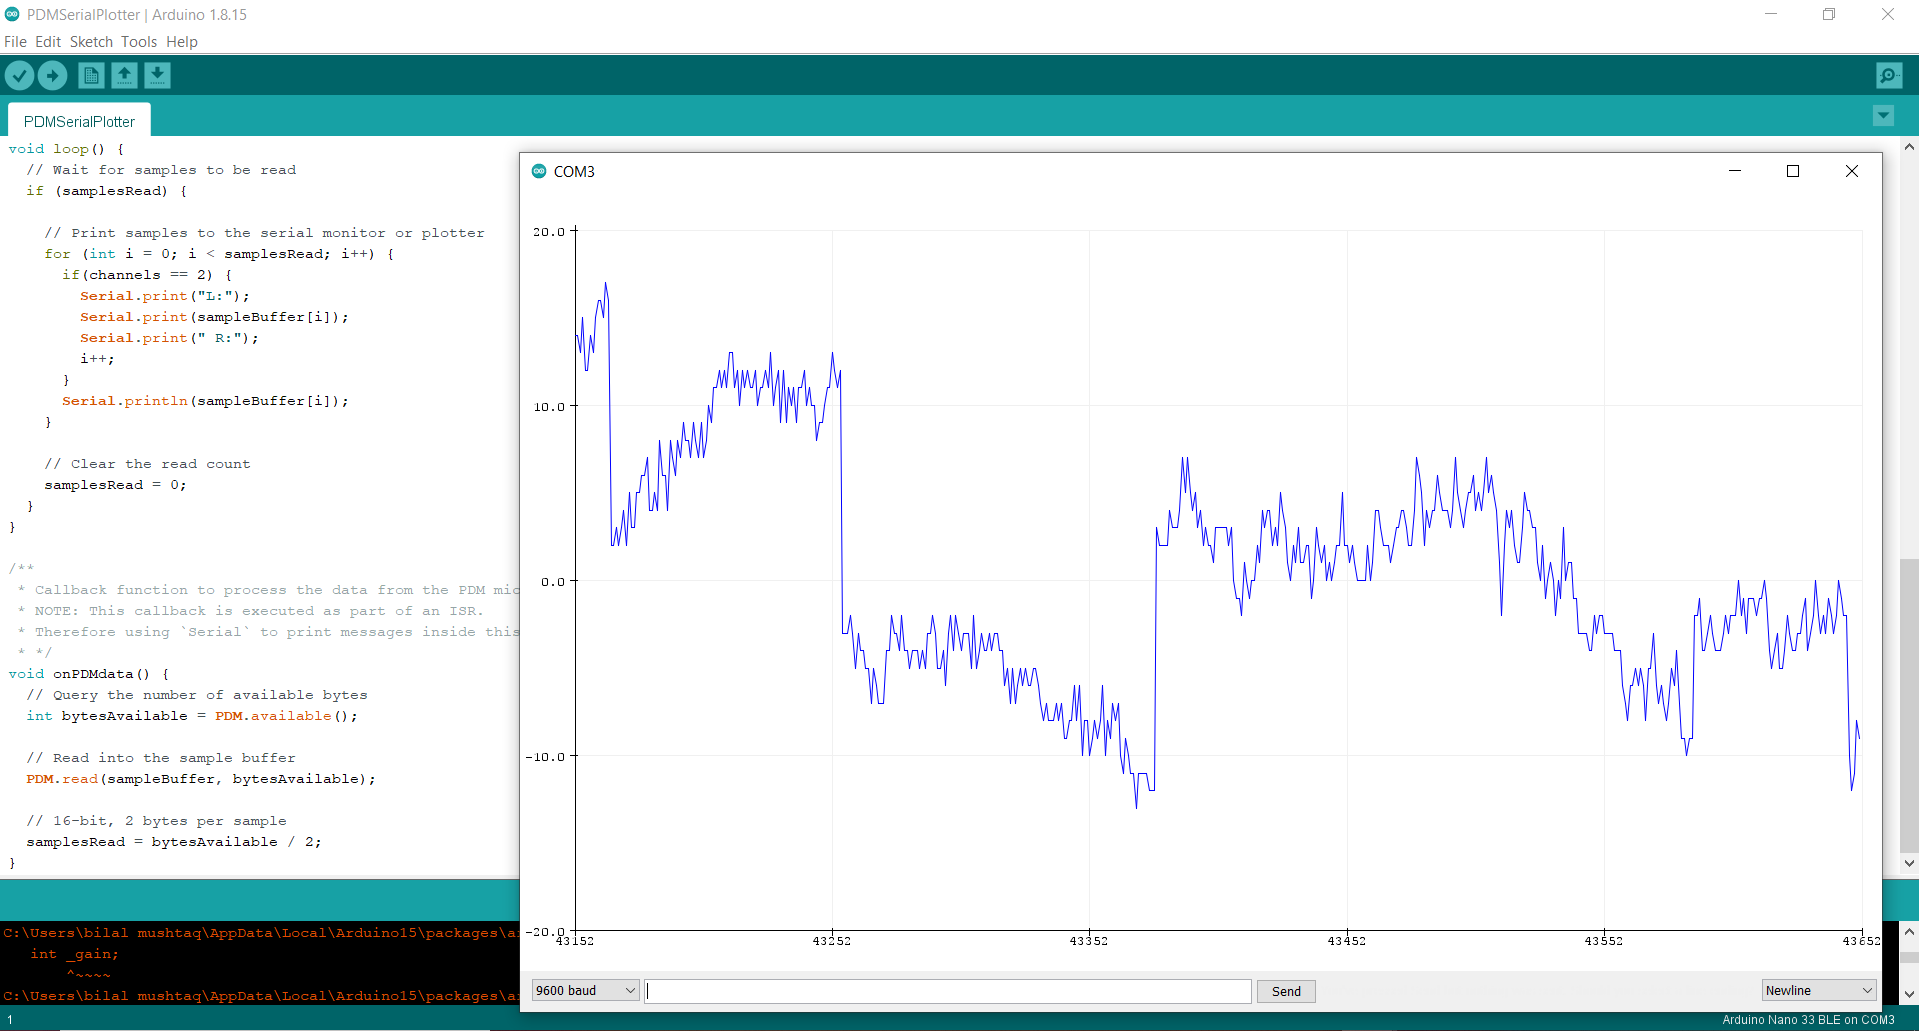
\includegraphics[width=8.5cm]{Nano33BLESense/10}
	\caption{MP34DT05, Serial Plotter}
	\label{fig:8}
\end{figure}

\section{Test with Bluetooth Module Connection}

The same procedure we need to follow for making the successful bleutooth coonection, the one we follow for on-board sensors. Below figure \ref{fig:testsoftware-fur-bluetooth} shows the ArduinoBLE library in the example section of Arduino IDE.



\begin{figure}[h]
	\centering
	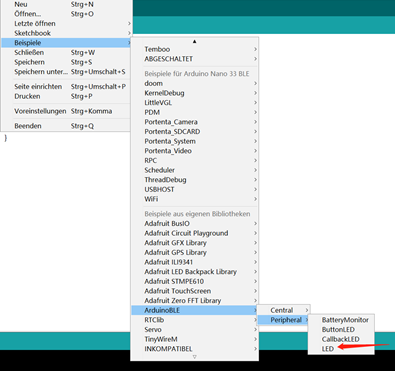
\includegraphics[width=0.7\linewidth]{Nano33BLESense/TestsoftwareBluetooth}
	\caption{Bluetooth Connection}
	\label{fig:testsoftware-fur-bluetooth}
\end{figure}

Bluetooth wireless technology allows us to share the data, the voice, the music, the video, and a lot of information between paired devices, It is built into many products, from mobile phones, cars to medical devices and computers. It has lower power consumption. It is easily upgradeable. It has range better than Infrared communication. Bluetooth is used for voice and data transfer, we can communicate by recieving and sending the data with other bluetooth connected devices. It is also possible to output a value on the phone side or also on the laptop by making the proper pairing. 




%%%%%%%%%%%%%%%
%
% $Autor: Wings $
% $Datum: 2020-01-29 07:55:27Z $
% $Pfad: komponenten/Bilderkennung/Produktspezifikation/Nano33BLESense/gpio.tex $
% $Version: 1785 $
%
% !TeX encoding = utf8
% !TeX root = Nano33BLESense
% !TeX TXS-program:bibliography = txs:///bibtex
%
%
%%%%%%%%%%%%%%%


%todo GitLab\ToDo\TinyML
% TinyML Seite 101

\chapter{Arduino}

Es gibt eine große Auswahl an Arduino-Boards, alle mit unterschiedlichen Fähigkeiten. Nicht auf allen läuft TensorFlow Lite für Mikrocontroller. Das Board, das nun verwendet wird, ist das Arduino Nano 33 BLE Sense. Es ist nicht nur mit TensorFlow Lite kompatibel, sondern enthält auch ein Mikrofon und einen Beschleunigungssensor. Wir empfehlen, die Version des Boards mit Headern zu kaufen, die es einfacher macht, andere Komponenten ohne Löten anzuschließen Die meisten Arduino-Boards haben eine eingebaute LED, und diese werden wir verwenden, um unsere Sinuswerte visuell auszugeben. Abbildung \ref{fig:NanoLED} zeigt ein Arduino Nano 33 BLE Sense-Board mit hervorgehobener LED.

\begin{figure}
  \centering
  \GRAPHICS{1.0}{1.0}{Nano33BLESense/timl_0602}
  
  \caption{ Arduino Nano 33 BLE Sense-Board mit hervorgehobener LED}\label{fig:NanoLED}
\end{figure}


 \section{Handhabung der Ausgabe am Arduino}
 
 Da wir nur mit einer LED arbeiten können, müssen wir kreativ denken. Eine Möglichkeit ist, die Helligkeit der LED basierend auf dem zuletzt vorhergesagten Sinuswert zu variieren.  Da der Wert von -1 bis 1 reicht, könnten wir 0 mit einer vollständig ausgeschalteten LED, -1 und 1 mit einer vollständig leuchtenden LED und alle Zwischenwerte mit einer teilweise gedimmten LED darstellen. Während das Programm in einer Schleife Schlussfolgerungen ausführt, wird die LED wiederholt ein- und ausgeblendet.

Mit der Konstante \PYTHON{kInferencesPerCycle} kann die Anzahl der Inferenzen, die über einen vollen Sinuszyklus durchgeführt werden, variiert werden. Da eine Inferenz eine bestimmte Zeit in Anspruch nimmt, kann durch die Einstellung der Konstante \PYTHON{kInferencesPerCycle}, die in \FILE{constants.cc} definiert ist, eingestellt werden, wie schnell die LED ausgeblendet wird.
 
Es gibt eine Arduino-spezifische Version dieser Datei in \FILE{hello\_world/arduino/constants.cc}. Die Datei hat den gleichen Namen wie \FILE{hello\_world/constants.cc}, so dass sie anstelle der ursprünglichen Implementierung verwendet wird, wenn die Anwendung für Arduino erstellt wird.
Um unsere eingebaute LED zu dimmen, können wir eine Technik namens Pulsweitenmodulation (PWM) verwenden. Wenn wir einen Ausgangspin extrem schnell ein- und ausschalten, wird die Ausgangsspannung des Pins zu einem Faktor des Verhältnisses zwischen der Zeit, die im Aus- und Ein-Zustand verbracht wird. Wenn der Pin 50 \% der Zeit in jedem Zustand verbringt, wird seine Ausgangsspannung 50 \% seines Maximums betragen. Wenn er 75 \% im Ein-Zustand und 25 \% im Aus-Zustand verbringt, wird seine Spannung 75 \% seines Maximums betragen.

PWM ist nur an bestimmten Pins bestimmter Arduino-Geräte verfügbar, aber es ist sehr einfach zu verwenden: Wir rufen einfach eine Funktion auf, die unseren gewünschten Ausgangspegel für den Pin festlegt.
 
 
     
 Der Code, der die Ausgabebehandlung für Arduino implementiert, befindet sich in \FILE{hello\_world/arduino/output\_handler.cc}, die anstelle der Originaldatei   \FILE{hello\_world/output\_handler.cc}.
 
 Gehen wir den Quellcode durch:
 
\begin{lstlisting}
 #include "tensorflow/lite/micro/examples/hello_world/output_handler.h"
 #include "Arduino.h"
 #include "tensorflow/lite/micro/examples/hello_world/constants.h"
\end{lstlisting} 


 Zunächst binden wir einige Header-Dateien ein. Unsere \FILE{output\_handler.h} spezifiziert die Schnittstelle für diese Datei. \FILE{Arduino.h} stellt die Schnittstelle für die Arduino-Plattform bereit; wir verwenden diese, um Steuerung des Boards. Da wir Zugriff auf \PYTHON{kInferencesPerCycle} benötigen, binden wir auch \FILE{constants.h}.
 
Als nächstes definieren wir die Funktion und weisen sie an, was sie bei der ersten Ausführung tun soll:

\begin{lstlisting}
 // Adjusts brightness of an LED to represent the current y value
 void HandleOutput(tflite::ErrorReporter* error_reporter, float x_value,
 float y_value) {
 	// Track whether the function has run at least once
 	static bool is_initialized = false;
 	// Do this only once
 	if (!is_initialized) {
 		// Set the LED pin to output
 		pinMode(LED_BUILTIN, OUTPUT);
 		is_initialized = true;
 	}
\end{lstlisting} 
 
 
In $C++$ behält eine Variable, die innerhalb einer Funktion als statisch deklariert ist, ihren Wert über mehrere Durchläufe der Funktion hinweg. Hier verwenden wir die Variable \PYTHON{is\_initialized}, um zu verfolgen, ob der Code in dem  folgenden Block \PYTHON{if (!is\_initialized)} jemals zuvor ausgeführt wurde.
     
Der Initialisierungsblock ruft die Funktion \PYTHON{pinMode()} von Arduino auf, die dem Mikrocontroller anzeigt, ob ein bestimmter Pin im Eingangs- oder Ausgangsmodus sein soll. Dies ist notwendig, bevor ein Pin verwendet wird. Die Funktion wird mit zwei von der Arduino-Plattform definierten Konstanten aufgerufen:  \PYTHON{LED\_BUILTIN} und \PYTHON{OUTPUT}.  \PYTHON{LED\_BUILTIN} steht für den Pin, der mit der eingebauten LED des Boards verbunden ist, und \PYTHON{OUTPUT} steht für den Ausgangsmodus.
     
Nachdem Sie den Pin der eingebauten LED auf den Ausgabemodus konfiguriert haben, setzen Sie \PYTHON{is\_initialized} auf \PYTHON{true}, damit dieser Blockcode nicht mehr ausgeführt wird.

Als Nächstes berechnen wir die gewünschte Helligkeit der LED:
     
     
\begin{lstlisting}
    // Calculate the brightness of the LED such that y=-1 is fully off
 	// and y=1 is fully on. The LED's brightness can range from 0-255.
 	int brightness = (int)(127.5f * (y_value + 1));
\end{lstlisting} 

Der Arduino erlaubt uns, den Pegel eines PWM-Ausgangs als Zahl von 0 bis 255 einzustellen, wobei 0 ganz aus und 255 ganz an bedeutet. Unser \PYTHON{y\_value} ist eine Zahl zwischen -1 und 1. Der vorhergehende Code ordnet \PYTHON{y\_value} dem Bereich 0 bis 255 zu, so dass bei y = -1 die LED ganz aus ist, bei y = 0 die LED halb leuchtet und bei y = 1 die LED ganz leuchtet.

Der nächste Schritt besteht darin, die Helligkeit der LED tatsächlich einzustellen:

\begin{lstlisting}
    // Set the brightness of the LED. If the specified pin does not support PWM,
 	// this will result in the LED being on when y > 127, off otherwise.
 	analogWrite(LED_BUILTIN, brightness);
\end{lstlisting} 

Die Funktion \PYTHON{analogWrite()} der Arduino-Plattform nimmt eine Pin-Nummer (wir geben \PYTHON{LED\_BUILTIN} an) und einen Wert zwischen 0 und 255. Wir geben unsere Helligkeit an, die in der vorherigen Zeile berechnet wurde. Wenn diese Funktion aufgerufen wird, leuchtet die LED mit dieser Helligkeit.


Leider ist bei einigen Modellen von Arduino-Boards der Pin, an dem die eingebaute LED angeschlossen ist, nicht PWM-fähig. Das bedeutet, dass unsere Aufrufe von \PYTHON{analogWrite()} seine Helligkeit nicht verändern werden. Stattdessen wird die LED eingeschaltet, wenn der in \PYTHON{analogWrite()} übergebene Wert über 127 liegt, und ausgeschaltet, wenn er 126 oder weniger beträgt.
     
Das bedeutet, dass die LED blinkt und ausschaltet, anstatt zu verblassen. Nicht ganz so cool, aber es demonstriert immer noch unsere Sinuswellenvorhersage.

Schließlich verwenden wir die \PYTHON{ErrorReporter}-Instanz, um den Helligkeitswert zu protokollieren:
     
\begin{lstlisting}
    // Log the current brightness value for display in the Arduino plotter
 	error_reporter->Report("%d\n", brightness);
\end{lstlisting}      
     
Auf der Arduino-Plattform ist der \PYTHON{ErrorReporter} so eingerichtet, dass er Daten über eine serielle Schnittstelle protokolliert. 	Die serielle Schnittstelle ist eine sehr verbreitete Art der Kommunikation zwischen Mikrocontrollern und Host-Computern und wird häufig für die Fehlersuche verwendet. Es ist ein Kommunikationsprotokoll, bei dem Daten bitweise durch Ein- und Ausschalten eines Ausgangspins übertragen werden. Wir können es verwenden, um alles zu senden und zu empfangen, von binären Rohdaten bis hin zu Text und Zahlen.
     
Die Arduino-IDE enthält Werkzeuge zum Erfassen und Anzeigen von Daten, die über eine serielle Schnittstelle empfangen werden. Eines der Werkzeuge, der Serial Plotter, kann ein Diagramm der Werte anzeigen, die er über die serielle Schnittstelle empfängt. Indem wir einen Strom von Helligkeitswerten aus unserem Code ausgeben, können wir sie grafisch darstellen. Abbildung \ref{fig:SerialPlotter} zeigt dies in Aktion.
 
\begin{figure}
    \centering
    \GRAPHICS{1.0}{1.0}{Nano33BLESense/timl_0603}
    
    \caption{Der serielle Plotter der Arduino-IDE}\label{fig:SerialPlotter}
\end{figure}
 	
 	
Eine Anleitung zur Verwendung des seriellen Plotters finden Sie weiter unten in diesem Abschnitt.
     
     
Sie fragen sich vielleicht, wie der \PYTHON{ErrorReporter} in der Lage ist, Daten über die serielle Schnittstelle des Arduino auszugeben. Sie finden die Code-Implementierung in \FILE{micro/arduino/debug\_log.cc}. Sie ersetzt die ursprüngliche Implementierung in \FILE{micro/debug\_log.cc}.

Genauso wie \FILE{output\_handler.cc} überschrieben wird, können wir plattformspezifische Implementierungen von jeder Quelldatei in TensorFlow Lite für Mikrocontroller bereitstellen, indem wir sie in ein Verzeichnis mit dem Namen der Plattform hinzufügen.

     
\section{Ausführen des Beispiels}
     
Unsere nächste Aufgabe besteht darin, das Projekt für Arduino zu erstellen und es auf einem Gerät einzusetzen. 	Es besteht immer die Möglichkeit, dass sich der Erstellungsprozess geändert hat, seit dieses Buch geschrieben wurde, daher sollten Sie in \href{https://oreil.ly/s2mj1}{README.md} nach den neuesten Anweisungen suchen.
     
Hier ist alles, was wir brauchen werden:

\begin{itemize}
    \item Ein unterstütztes Arduino-Board (wir empfehlen das Arduino Nano 33 BLE Sense)
    \item Das passende USB-Kabel 
    \item Die Arduino IDE (Sie müssen diese herunterladen und installieren, bevor Sie fortfahren)
\end{itemize}
     
 Die Projekte in diesem Buch sind als Beispielcode in der TensorFlow Lite Arduino-Bibliothek verfügbar, die Sie einfach über die Arduino-IDE und die Auswahl von Manage Libraries aus dem Tools-Menü installieren können. Suchen Sie im erscheinenden Fenster nach der Bibliothek mit dem Namen \PYTHON{Arduino\_TensorFlowLite} und installieren Sie sie. Sie sollten in der Lage sein, die neueste Version zu verwenden, aber wenn Sie auf Probleme stoßen, ist die Version, die mit diesem Buch getestet wurde, 1.14-ALPHA.
     
Sie können die Bibliothek auch aus einer .zip-Datei installieren, die Sie entweder vom TensorFlow Lite Team \href{https://oreil.ly/blgB8}{download} oder mit dem TensorFlow Lite for Microcontrollers Makefile selbst erzeugen können. Wenn Sie dies bevorzugen, lesen Sie bitte Anhang A.

Nachdem Sie die Bibliothek installiert haben, wird das Beispiel im Menü File unter \FILE{Examples$\rightarrow$\_Arduino\_TensorFlowLite\_} angezeigt, wie in Abbildung \ref{fig:ArduIDE} gezeigt.	

\begin{figure}
    \centering
    \GRAPHICS{0.5}{1.0}{Nano33BLESense/timl_0604}
    
    \caption{Der serielle Plotter der Arduino-IDE}\label{fig:ArduIDE}
\end{figure}
 	
Klicken Sie auf ``hello\_world'', um das Beispiel zu laden. Es wird als neues Fenster mit einer Registerkarte für jede der Quelldateien angezeigt. Die Datei in der ersten Registerkarte, \FILE{hello\_world}, entspricht der \FILE{main\_functions.cc}, die wir vorhin durchgegangen sind.
 
\section{Differences in the Arduino Example Code}
     
Wenn die Arduino-Bibliothek generiert wird, werden einige kleinere Änderungen am Code vorgenommen, damit er gut mit der Arduino-IDE funktioniert. Das bedeutet, dass es einige subtile Unterschiede zwischen dem Code in unserem Arduino-Beispiel und im TensorFlow GitHub Repository gibt. Zum Beispiel werden in der Datei \FILE{hello\_world} die Funktionen \PYTHON{setup()} und \PYTHON{loop()} automatisch von der Arduino Umgebung aufgerufen, so dass die Datei \FILE{main.cc} und ihre Funktion \PYTHON{main()} nicht benötigt werden.

Die Arduino-IDE erwartet außerdem, dass die Quelldateien die Erweiterung .cpp anstelle von .cc haben. Da die Arduino-IDE keine Unterordner unterstützt, wird außerdem jedem Dateinamen im Arduino-Beispiel der ursprüngliche Name des Unterordners vorangestellt. Zum Beispiel entspricht \FILE{arduino\_constants.cpp} der ursprünglich benannten Datei \FILE{arduino/constants.cc}.

Abgesehen von ein paar kleinen Unterschieden bleibt der Code jedoch weitgehend unverändert.
 
Um das Beispiel auszuführen, schließen Sie Ihr Arduino-Gerät über USB an. Stellen Sie sicher, dass der richtige Gerätetyp in der Dropdown-Liste ``Board'' im Menü ``Tools'' ausgewählt ist, wie in Abbildung \ref{fig:ArduSelectBoard} gezeigt. 	
 	
\begin{figure}
    \centering
    \GRAPHICS{1.0}{1.0}{Nano33BLESense/timl_0605}
    
    \caption{Die Dropdown-Liste Board}\label{fig:ArduSelectBoard}
\end{figure}     
     
Wenn der Name Ihres Geräts nicht in der Liste erscheint, müssen Sie sein Support-Paket installieren. Klicken Sie dazu auf Boards Manager. Suchen Sie in dem daraufhin angezeigten Fenster nach Ihrem Gerät und installieren Sie die neueste Version des entsprechenden Support-Pakets.

Stellen Sie anschließend sicher, dass der Anschluss des Geräts in der Dropdown-Liste ``Anschluss'' ausgewählt ist, die sich ebenfalls im Menü ``Tools'' befindet (siehe Abbildung  \ref{fig:ArduSelectPort}).

\begin{figure}
    \centering
    \GRAPHICS{1.0}{1.0}{Nano33BLESense/timl_0606}
    
    \caption{Die Dropdown-Liste Port}\label{fig:ArduSelectPort}
\end{figure} 


Klicken Sie schließlich im Arduino-Fenster auf die Schaltfläche Upload (in Abbildung \ref{fig:ArduUpload} weiß hervorgehoben), um den Code zu kompilieren und auf Ihr Arduino-Gerät hochzuladen.

\begin{figure}
    \centering
    \GRAPHICS{1.0}{1.0}{Nano33BLESense/timl_0607}
    
    \caption{Die Upload-Schaltfläche, ein nach rechts gerichteter Pfeil}\label{fig:ArduUpload}
\end{figure} 


Nachdem der Upload erfolgreich abgeschlossen wurde, sollten Sie sehen, dass die LED auf Ihrem Arduino-Board beginnt, entweder ein- und auszublenden oder ein- und auszublinken, je nachdem, ob der Pin, an den sie angeschlossen ist, PWM unterstützt.

\medskip

Glückwunsch: Sie führen ML auf dem Gerät aus!

\medskip


Verschiedene Modelle von Arduino-Boards haben unterschiedliche Hardware und führen die Inferenz mit unterschiedlichen Geschwindigkeiten aus. Wenn Ihre LED entweder flackert oder komplett an bleibt, müssen Sie möglicherweise die Anzahl der Inferenzen pro Zyklus erhöhen. Sie können dies über die Konstante \PYTHON{kInferencesPerCycle} in \FILE{arduino\_constants.cpp} tun.



 	"Eigene Änderungen vornehmen" auf Seite 111 zeigt Ihnen, wie Sie den Code des Beispiels bearbeiten können.


Sie können den Helligkeitswert auch in einem Diagramm darstellen. Öffnen Sie dazu den seriellen Plotter der Arduino-IDE, indem Sie ihn im Menü "Tools" auswählen, wie in Abbildung \ref{fig:ArduSerial} gezeigt.

\begin{figure}
    \centering
    \GRAPHICS{1.0}{1.0}{Nano33BLESense/timl_0608}
    
    \caption{Der Menüpunkt Serieller Plotter}\label{fig:ArduSerial}
\end{figure} 


Der Plotter zeigt den Wert an, wie er sich über die Zeit ändert, wie in Abbildung \ref{fig:ArduSerialGraph} gezeigt. 

\begin{figure}
    \centering
    \GRAPHICS{1.0}{1.0}{Nano33BLESense/timl_0603}
    
    \caption{Der Serienplotter, der den Wert grafisch darstellt}\label{fig:ArduSerialGraph}
\end{figure} 



Um die Rohdaten zu betrachten, die von der seriellen Schnittstelle des Arduinos empfangen werden, öffnen Sie den Serial Monitor aus dem Menü Tools. Sie sehen dann einen Strom von Zahlen vorbeifliegen, wie in Abbildung \ref{fig:ArduSerialRaw}.

\begin{figure}
    \centering
    \GRAPHICS{1.0}{1.0}{Nano33BLESense/timl_0610}
    
    \caption{Der Serial Monitor zeigt Rohdaten an}\label{fig:ArduSerialRaw}
\end{figure} 
	
 	
\section{Eigene Änderungen vornehmen}

Jetzt, wo Sie die Anwendung bereitgestellt haben, macht es vielleicht Spaß, herumzuspielen und einige Änderungen am Code vorzunehmen. Sie können die Quelldateien in der Arduino-IDE bearbeiten. Wenn Sie speichern, werden Sie aufgefordert, das Beispiel an einem neuen Ort zu speichern. Wenn Sie mit den Änderungen fertig sind, können Sie in der Arduino-IDE auf die Schaltfläche ``Hochladen'' klicken, um das Beispiel zu erstellen und bereitzustellen.

Um mit dem Vornehmen von Änderungen zu beginnen, können Sie einige Experimente durchführen:

\begin{itemize}
  \item Lassen Sie die LED langsamer oder schneller blinken, indem Sie die Anzahl der Inferenzen pro Zyklus anpassen.
  \item  Ändern Sie \FILE{output\_handler.cc}, um eine textbasierte Animation an der seriellen Schnittstelle zu protokollieren.
  \item  Verwenden Sie die Sinuswelle, um andere Komponenten zu steuern, z. B. zusätzliche LEDs oder Tongeneratoren.
\end{itemize}
 	
 	
 	


%%%
%
% $Autor: Wings $
% $Datum: 2021-05-14 $
% $Pfad: GitLab/MLEdgeComputer $
% $Dateiname: CAMov2640 
% $Version: 4620 $
%
% !TeX spellcheck = de_GB
%
%%%

\chapter{Sensor ov2640}

\url{https://www.arducam.com/ov2640/}

\url{https://www.arducam.com/focal-length-calculator/}

\section{Produktbeschreibung}

Arducam-M-2MP ist eine optimierte Version von Arducam Shield Rev.C und ist eine hochauflösende 2MP-SPI-Kamera, die die Komplexität der Kamerasteuerung verringert. Sie verfügt über einen 2-MP-CMOS-Bildsensor OV2640 und hat eine Miniaturgröße sowie eine einfach zu bedienende Hardware-Schnittstelle und die Open-Source-Code-Bibliothek. Die Arducam Mini-Kamera kann auf allen Plattformen wie Arduino, Raspberry Pi, Maple, Chipkit, Beaglebone Black verwendet werden, solange sie über eine SPI- und I2C-Schnittstelle verfügen und mit Standard-Arduino Boards verbunden werden können. Die Arducam Mini-Kamera bietet nicht nur die Möglichkeit, eine Kamera-Schnittstelle hinzuzufügen, die in einigen Mikrocontrollern nicht vorhanden ist, sondern bietet auch die Möglichkeit, mehrere Kameras zu einem einzigen Mikrocontroller hinzuzufügen.

\bigskip

Anwendung:
\begin{itemize}
  \item IoT-Kameras.
  \item Roboterkameras.
  \item Wildlife-Kameras.
\end{itemize}

Andere batteriebetriebene Produkte.
Kann auf Plattformen wie MCU, Raspberry Pi, ARM, DSP, FPGA verwendet werden.

\bigskip

Eigenschaften:

\begin{itemize}
  \item 2-Megapixel-Bildsensor OV2640.
  \item M12-Mount- oder CS-Mount-Objektivhalter mit wechselbaren Objektivoptionen.
  \item IR-empfindlich mit entsprechender Objektivkombination.
  \item I2C-Schnittstelle für die Sensorkonfiguration.
  \item SPI-Schnittstelle für Kamera-Befehle und Datenstrom.
  \item Alle E/A-Anschlüsse sind für 5 V/3,3 V geeignet.
  \item Unterstützt JPEG-Komprimierungsmodus, Einzel- und Mehrfachaufnahmemodus, einmaliges Erfassen mehrerer Lesevorgänge, Burst-Lese-Operation, Niedrige-Energie-Modus usw..
  \item Kann mit Standard-Arduino-Boards verbunden werden.
  \item Open-Source-Code-Bibliothek für Arduino, STM32, Chipkit, Raspberry Pi, BeagleBone Black.
  \item Schlanke Form.
\end{itemize}

\bigskip

Lieferumfang:

1 x Arducam Mini-Modul Kameraschutz mit OV2640 2 MP, Objektiv, für Arduino UNO Mega2560 Board.

Hinweis: Arduino UNO ist nicht enthalten.

\bigskip


\url{https://www.amazon.com/dp/B07D58GDDV/ref=sr_1_17_sspa?__mk_de_DE=ÅMÅŽÕÑ&dchild=1&keywords=arducam&qid=1622358684&sr=8-17-spons&psc=1&spLa=ZW5jcnlwdGVkUXVhbGlmaWVyPUEyWUdNSVhJSFNUQUtLJmVuY3J5cHRlZElkPUEwNjI4NTQxM0RNQ0I2NDJDNzdUTCZlbmNyeXB0ZWRBZElkPUEwMjEyMjUwNTFSVjM2SzZFM1VCJndpZGdldE5hbWU9c3BfYXRmX25leHQmYWN0aW9uPWNsaWNrUmVkaXJlY3QmZG9Ob3RMb2dDbGljaz10cnVl0}

    
Raspberry Pi Kamerakabel, iUniker 15-poliges Flachbandkabel, Pi Kamera Flex Kabel, Flex CSI Kabel 50 cm/1 m/2 m für Raspberry Pi 3B+, 3B, 2B (nicht für Pi Zero)
    
\begin{figure}
    \begin{center}
        \includegraphics[scale=0.13]{CAM/ov2640/ov2640}
        \quad 
        \includegraphics[scale=0.15]{CAM/ov2640/ov2640B4}
        
        \caption{Kamera IMX477 der Firma Arducam; \cite{Arducam:2021}}
    \end{center}    
\end{figure}



\section{ArduCAM Library Introduction}

\url{https://github.com/ArduCAM/Arduino}


Dies ist eine Open-Source-Bibliothek für die Aufnahme von hochauflösenden Standbildern und kurzen Videoclips auf Arduino-basierten Plattformen unter Verwendung der Kameramodule von ArduCAM.
Die Kamera-Breakout-Boards sollten vor dem Anschluss an die Arduino-Boards mit dem ArduCAM-Shield funktionieren.
ArduCAM-Kameramodule der Mini-Serie wie Mini-2MP, Mini-5MP(Plus) können direkt an Arduino-Boards angeschlossen werden.
Zusätzlich zu Arduino kann die Bibliothek auf beliebige Hardware-Plattformen portiert werden, solange sie über eine I2C- und SPI-Schnittstelle verfügen, die auf dieser ArduCAM-Bibliothek basiert.

\bigskip

Now Supported Cameras

\begin{itemize}
  \item OV7660 0.3MP
  \item OV7670 0.3MP
  \item OV7675 0.3MP
  \item OV7725 0.3MP
  \item MT9V111 0.3MP
  \item MT9M112 1.3MP
  \item MT9M001 1.3MP
  \item MT9D111 2MP
  \item OV2640 2MP JPEG
  \item MT9T112 3MP
  \item OV3640 3MP
  \item OV5642 5MP JPEG
  \item OV5640 5MP JPEG
\end{itemize}

Supported MCU Platform

Theoretically support all Arduino families

\begin{itemize}
  \item Arduino UNO R3 (Tested)
  \item Arduino MEGA2560 R3 (Tested)
  \item Arduino Leonardo R3 (Tested)
  \item Arduino Nano (Tested)
  \item Arduino DUE (Tested)
  \item Arduino Genuion 101 (Tested)
  \item Raspberry Pi (Tested)
  \item ESP8266-12 (Tested) (\url{http://www.arducam.com/downloads/ESP8266_UNO/package_ArduCAM_index.json})
  \item Feather M0 (Tested with OV5642)
\end{itemize}


Note: ArduCAM library for ESP8266 is maintained in another repository ESP8266 using a json board manager script.


\section{Libraries Structure}

Die Basisbibliotheken bestehen aus zwei Unterbibliotheken: \FILE{ArduCAM} und \FILE{UTFT4ArduCAM\_SPI}. Diese beiden Bibliotheken sollten direkt unter die Bibliotheken des Arduino-Verzeichnisses kopiert werden, damit sie von der Arduino-IDE erkannt werden.

Die ArduCAM-Bibliothek ist die Kernbibliothek für ArduCAM-Shields. Sie enthält unterstützte Bildsensortreiber und Benutzerland-API-Funktionen, die Befehle zum Erfassen oder Lesen von Bilddaten erteilen. Es gibt auch ein Beispielverzeichnis innerhalb der ArduCAM-Bibliothek, das die meisten Funktionen der ArduCAM-Shields illustriert. Die vorhandenen Beispiele sind Plug-and-Play, ohne dass eine einzige Zeile Code geschrieben werden muss.

Die Bibliothek \FILE{UTFT4ArduCAM\_SPI} ist eine modifizierte Version von UTFT, die von Henning Karlsen geschrieben wurde. Wir haben sie portiert, um das ArduCAM-Shield mit LCD-Bildschirm zu unterstützen. Daher wird die Bibliothek \FILE{UTFT4ArduCAM\_SPI} nur benötigt, wenn das ArduCAM-LF-Modell verwendet wird.




\section{How to use}

Die Bibliotheken sollten vor dem Ausführen von Beispielen konfiguriert werden, andernfalls erhalten Sie eine Fehlermeldung beim Kompilieren.

\subsection{1. Edit \FILE{memorysaver.h} file}

Öffnen Sie die Datei \FILE{memorysaver.h} im ArduCAM-Ordner und aktivieren Sie die Hardwareplattform und das Kameramodul, das zu Ihrer Hardware passt, indem Sie die Makrodefinition in der Datei auskommentieren oder auskommentieren. Wenn Sie zum Beispiel eine ArduCAM-Mini-2MP haben, sollten Sie die Zeile \PYTHON{\#define OV2640\_MINI\_2MP} auskommentieren und alle anderen Zeilen auskommentieren. Und wenn Sie ein ArduCAM-Shield-V2 und ein OV5642-Kameramodul haben, sollten Sie die Zeile \PYTHON{\#define ARDUCAM\_SHIELD\_V2} und die Zeile \PYTHON{\#define OV5642\_CAM} auskommentieren und dann alle anderen Zeilen.

\subsection{2. Choose correct CS pin for your camera}

Öffnen Sie eines der Beispiele und verdrahten Sie die SPI- und I2C-Schnittstelle, insbesondere die CS-Pins, entsprechend den Beispielen mit dem ArduCAM-Shield. Hardware und Software sollten konsistent sein, um die Beispiele korrekt auszuführen.

\subsection{3. Upload the examples}


Im Beispielordner befinden sich sieben Unterverzeichnisse für verschiedene ArduCAM-Modelle und die Host-Anwendung. Der Ordner Mini ist für die Module ArduCAM-Mini-2MP und ArduCAM-Mini-5MP.

\begin{enumerate}
  \item Der Ordner \FILE{Mini\_5MP\_Plus} ist für ArduCAM-Mini-5MP-Plus (OV5640/OV5642) Module.
  \item Der Ordner \FILE{RevC} ist für ArduCAM-Shield-RevC oder ArduCAM-Shield-RevC+ Shields.
  \item Der Ordner \FILE{Shield\_V2} ist für das ArduCAM-Shield-V2 Schild.
  \item Der Ordner \FILE{host\_app} ist die Host-Erfassungs- und Anzeigeanwendung für alle ArduCAM-Module.
  \item Der Ordner \FILE{RaspberryPi} ist eine Beispielanwendung für die Raspberry Pi-Plattform, siehe weitere Anleitung.
  \item Der Ordner \FILE{ESP8266} ist für ArduCAM-ESP8266-UNO-Board-Beispiele für Bibliothekskompatibilität. Bitte versuchen Sie stattdessen, ESP8266 mit dem Skript josn board manager zu repositoryen.
\end{enumerate}


Selecting correct COM port and Arduino boards then upload the sketches.

\bigskip

     
Arducam MINI Kamera Demo Tutorial für Arduino

Arducam Kamera-Schild V2 Demo Tutorial für Arduino

\subsection{4. How To Connect Bluetooth Module}
Mit dieser Demo

\url{https://github.com/ArduCAM/Arduino/blob/master/ArduCAM/examples/mini/ArduCAM_Mini_Video_Streaming_Bluetooth}

So laden Sie den Host V2:

% \Ausblenden
{

\begin{itemize}
  \item For ArduCAM\_Host\_V2.0\_Mac.app, please refer to this link:
  
         \url{www.arducam.com/downloads/app/ArduCAM_Host_V2.0_Mac.app.zip}
  \item For ArduCAM\_Mini\_V2.0\_Linux\_x86\_64bit, Please refer to this link:
       
       \url{www.arducam.com/downloads/app/ArduCAM_Mini_V2.0_Linux_x86_64bit.zip}
\end{itemize}

}

%%%%%%%
%
% $Autor: Wings $
% $Datum: 2021-05-14 $
% $Pfad: GitLab/MLEdgeComputer/Portenta $
% $Dateiname: VisionShield
% $Version: 4620 $
%
%%%%%%



\section{ArduCAM Mini-Kameramodul mit 2MP Plus OV2640 für Arduino}


\begin{figure}
	\centering
  \includegraphics[width=0.4\textwidth]{Arduino/ArduCAM2MP}
\caption{ArduCAM Mini-Kameramodul mit 2MP Plus OV2640 für Arduino \href{https://store.arduino.cc/portenta-h7}{Arduino Store}}
\end{figure}


\url{https://www.robotshop.com/de/de/arducam-mini-kameramodul-mit-2mp-plus-ov2640-arduino.html}

\url{https://www.arducam.com/product/arducam-2mp-spi-camera-b0067-arduino/}



%%%
%
% $Autor: Wings $
% $Datum: 2021-05-14 $
% $Pfad: GitLab/MLEdgeComputer $
% $Dateiname: LensCalibrationTool
% $Version: 4620 $
%
% !TeX spellcheck = de_DE/GB
%
%%%



\chapter{Lens Calibration Tool}


Arducam Lens Calibration Tool, Sichtfeld (Field of View, FoV) Test Chart Folding Card, Pack of 2

\url{https://www.amazon.com/-/de/dp/B0872Q1RLD/ref=sr_1_40?__mk_de_DE=ÅMÅŽÕÑ&dchild=1&keywords=arducam&qid=1622358908&sr=8-40}

\begin{description}
  \item[Multifunktional für Objektiv:] Objektivfokus kalibrieren, FoV messen und Schärfe abschätzen
  \item[Einfach zu bedienen:] Schnelle Einrichtung in Sekunden und Messung in Minuten mit Online-Videotutorial.
  \item[Ein handliches Werkzeug:] Einfaches Ermitteln des Sichtfelds des Objektivs ohne Berechnung
  \item[Sauber und aufgeräumt:] Faltbarer Kartenstil, mehrfach gefaltet und aufgerollt für schnelle Einstellung und bessere Lagerung
  \item[Anwendung:] Fokuskalibrierung, Schärfeschätzung und Bildfeld-Schnellmessung für M12, CS-Mount, C-Mount und DSLR-Objektive.

\end{description}
\url{https://www.arducam.com/product/arducam-lens-calibration-tool-field-of-view-fov-test-chart-folding-card-pack-of-2/}


\begin{figure}
  \begin{center}
    \includegraphics[scale=0.15]{CAM/LensCalibrationTool/LensCalibrationTool}
    \quad 
    \includegraphics[scale=0.1]{CAM/LensCalibrationTool/LensCalibrationTool4}
  
    \caption{Kalibrierungswerkzeug der Firma Arducam; \cite{Arducam:2021}}
  \end{center}    
\end{figure}

\section{Übersicht}

Sind Sie immer noch frustriert von der Berechnung des FOV Ihrer Objektive und den unscharfen Bildern? Arducam hat jetzt ein multifunktionales Tool für Objektive veröffentlicht, mit dem Sie das Sichtfeld des Objektivs ohne Berechnung erhalten und den Objektivfokus schnell und einfach kalibrieren können.

\section{Applications}

Focus calibration, sharpness estimation and field of view quick measuring for M12, CS-Mount, C-Mount, and DSLR lenses

\section{Package Contents}

2*Foldable Lens Calibration Card




%%%%%%%%%%%%
%
% $Autor: Wings $
% $Datum: 2019-03-05 08:03:15Z $
% $Pfad: Automatisierung/Skript/Produktspezifikation/Powerpoint/AMF.tex $
% $Version: 4250 $
% !TeX spellcheck = en_GB/de_DE
% !TeX encoding = utf8
% !TeX root = filename 
% !TeX TXS-program:bibliography = txs:///biber
%
%%%%%%%%%%%%

\chapter{Project Implementation Steps}

The main focus to implement this project is to train the Arduino Nano 33 BLE Sense for edge computing application. The edge computer will behave and react as the human do after deploying machine learning algorithm and computer vision technique. These are the following outputs we need for completing this project \href{https://www.edgeimpulse.com/}{[Edge Impulse]}.
\begin{itemize}
	\item Gesture Detection
	\item Object Detection
	\item Color Detection
\end{itemize}
Initially I have tried multiple technique to implement the color and object detection part of this project. One of them is Edge Impulse.

\section{Edge Impulse}
Edge Impulse was designed for software developers, engineers and domain experts to solve real problems using machine learning on edge devices without a prior in machine learning. I have tried this platform for color detection, Key word detection, and object detection but later I have switched to other techiques too.Fig\ref{Edge Impulse Flow Chart} shows the different steps involve for training the model.  
\begin{figure}[h]
	\centering
	\includegraphics[width=0.6\linewidth]{Nano33BLESense/Edge Impulse}
	\caption{Edge Impulse Flow Chart}
	\label{Edge Impulse Flow Chart}
\end{figure}
Edge impulse can be the great start for beginner, it allow us to make the data set and also assit us during the whole procedure. This platform support particular type of edge computer, Arduino Nano 33 BLE Sense is also one of them.For getting start with edge impulse we need to make a account on edge impulse website. \href{https://www.edgeimpulse.com/}{[Edge Impulse]}.
\begin{itemize}
	\item Edge Impulse is the leading development platform for embedded
	machine learning.
	\item It supports number of embedded hardwares including (Arduin Nano
	33 BLE Sense).
	\item Help us to create data set for Machine learning model.
	\item Shows the uncertainty in data.
	\item Split the data into training (80 percent) and test (20 percent).
	\item Predict the most suitable Machine learning algorithm to train the
	model.
	\item Allow us to test the model and see the accuracy.
	\item After doing all these above steps, we can deploy the train model in
	our Arduino nano 33 BLE Sense
\end{itemize}

\section{Gesture Detection}
Gesture detection is the main task for doing this project. On the basis of different gestures we need to train the Arduino Nano 33 BLE Sense to behave differently on each gesture. My task is cto define the type of gesture what I want to detect, and also recognize these gestures for getting the certain output from Arduino Nano 33 BLE Sense.
\subsection{First Approach for Gesture Detection}
During my research, while going through for defining the type of gestures, I have found very few solutions. One of the most visible solution is the available sensor on Arduino Nano 33 BLE Sense is APDS9960. This sensor can detect four different types of gesture (Moving left, Moving right, Up, Down) these 4 gesture sense the sensor when i move my hand in front of sensor. This was the first solution, and the available library and code is also available in the arduino IDE. I was not satisfy with this solution, because every time the sensor sense the movement when I put my hand very close to the sensor approximately 15mm. So, I switch from sensor detection to Computer vision and Machine learning techniques.
\section{Gesture Detection Test Using MediaPipe}
MediaPipe is the framework in computer vision and support so many Machine learning algorithm to make usefull application. It help us to define to gesture using hand by making the gesture on the basis of hand landmarks. Initially as a test, I have tried to count the finger of hand and show them on the computer using the OpenCV and MediaPipe module. It is detecting very fast and accurate with good frame per second (FPS). Fig\ref{Counting Finger Using MediaPipe and OpenCV} shows the result of counting finger using the MediaPipe technique on the basis of hand landmarks.
\begin{figure}[h]
	\centering
	\includegraphics[width=0.5\linewidth]{Nano33BLESense/MediaPipe Check}
	\caption{Counting Finger Using MediaPipe and OpenCV}
	\label{Counting Finger Using MediaPipe and OpenCV}
\end{figure}

\subsection{Successful Approach of Gesture Detection} 
For gesture detection, I choose my hand to define the different types of gesture for edge devices. The most suitable module I found for this is MediaPipe, it help me to make the different types of gesture using the hand landmarks. \href{https://google.github.io/mediapipe/solutions/hands.html}{MediaPipe Hand Landmark Solution} There are 21 hand Landmarks on each hand, we can use the both hand for making the more complex gesture too by changing the position of our fingures or even the individual landmark on hand. Fig\ref{Hand Landmarks using MediaPipe} shows the 21 3D hand landmarks.
\begin{figure}[h]
	\centering
	\includegraphics[width=0.6\linewidth]{Nano33BLESense/Hand Landmarks}
	\caption{Hand Landmarks using MediaPipe}
	\label{Hand Landmarks using MediaPipe}
\end{figure}
MediaPipe module uses the convolutional neural network and took 30,000 3D images to train this module. It has very good accuracy and precision, there are some functions written in this module to detect which landmarks we want to detect. Fig\ref{Hand Landmarks using MediaPipe Function} shows for detecting the 21 hand landmarks of the hand are:

\begin{figure}[h]
	\centering
	\includegraphics[width=0.7\linewidth]{Nano33BLESense/Landmarks}
	\caption{Hand Landmarks using MediaPipe Function}
	\label{Hand Landmarks using MediaPipe Function}
\end{figure}
With the help of these hand landmarks, we can define the different types of gestures. For example by opening or closing the finger we are able to define and detect gestures or by changing the position of landmarks, by changing position the landmarks also changes the x and y value. MediaPipe help us to detect these changes and also recognize it for getting certain output. The Following two solution I have tried this with the help of MediaPipe Hand Landmarks detection are:
\subsection{Gesture Detection on Arduino Nano 33 BLE Sense}
For doing the Gesture detection on Arduino Nano 33 BLE Sense, I used the following set of Software, framework, Libraries, Modules and Hardwares.
\begin{itemize}
	\item Arduino IDE
	\item Pycharm
	\item Logitech Camera
	\item MediaPipe Algorithm
	\item OpenCV
	\item Pyfirmata
\end{itemize}  
These are the sets of hardware and software pieces I have used for detecting the gestures with Arduino Nano 33 BLE Sense. For the detection part I have define six different outputs on each six different gesture detection. The outputs are (Run, Stop, Slow, Fast, Turn Left, Turn Right). I wrote the Python program in Pycharm software, because MediaPipe module is written in python. Arduino IDE is support only c++, and it is not directly support python libraries and module. Pyfirmata use for seriel communication protocol between python supportive host computer and embedded device have Arduino IDE. By Installing pyfirmata we are able to run the python program on host computer and by serial communication get the results on Arduino Nano 33 BLE Sense. 
Similarly Logitech camera is for capturing the gesture, I have switch to Logitech camera for better resolution and pixels. OpenCV library use for better visualization, writing color function making circles and image processing.
\subsection{Gesture Detection Results On Arduino Nano 33 BLE Sense}
There are six different types of Gestures define and detect by using Hand landmark function of MediaPipe module. The detected signs on the basis of gestures are (Run, Stop, Fast, Slow, Please Turn Left, Please Turn Right). These signs are detect by using the landmarks of hand, and we can define and detect as many gesture by using hand landmark technique. Fig\ref{Gesture Detection on Arduino} shows the detected gestures and sign results are as follow.
\begin{figure}[h]
	\centering
	\includegraphics[width=0.7\linewidth]{Nano33BLESense/Arduino Gesture}
	\caption{Gesture Detection on Arduino}
	\label{Gesture Detection on Arduino}
\end{figure}
\section{Gesture Detection Using LSTM Layer and Tensor Flow}
This Model is also equally perform well for detecting the gestures for high processing power computers. The Following sets of Libraries, Software, Module, Hardware, and Packages.
\begin{itemize}
	\item Anaconda (For Jupyter Notebook)
	\item Numpy
	\item Matplotlib
	\item sklearn
	\item TensorFlow 2.6
	\item OpenCV
	\item MediaPipe
	\item CUDA 11.0 
	\item Cudnn 8.2
\end{itemize}
For training the model  I have used the LSTM layer, with Tensorflow for MediaPipe gesture detection. It also detect different types of sign on different gestures. The gestures detect the following five sign (Run, Stop, Slow, Fast, Going Good). I have tried 2000 epochs for training the model but this technique gives the 99 percent accuracy after 300 epochs.
\subsection{Gesture Detection Results Using LSTM and TensorFlow using MediaPipe}
The similar type of gesture detection technique has been tried with long short term memory (LSTM) layer and TensorFlow framework. The model is trained for 5 different classes, (Run, Fast, Slow, Stop, and Going Good(GGood)), these gestures are also detecting using MediaPipe hand Landmarks technique. Fig\ref{Gesture Detection Using LSTM, TensorFlow, and MediaPipe} shows the result of train model detecting the different gestures.
\begin{figure}[h]
	\centering
	\includegraphics[width=0.7\linewidth]{Nano33BLESense/LSTM Results}
	\caption{Gesture Detection Using LSTM, TensorFlow, and MediaPipe}
	\label{Gesture Detection Using LSTM, TensorFlow, and MediaPipe}
\end{figure}
\section{Color Detection}
For this project, the task is to detect the Red, Green, Blue (RGB) color for different product. In the Arduino Nano 33 BLE Sense, there is on-board sensor APDS9960 whose one of the function is also to detect RGB color. I used this sensor and it give us the RGB percentage of each color in the product. The available program and library is also available in the Arduino IDE for executing this programm.
\section {Object Detection}
There are multiple solution I have tried for object detection too, one with the MediaPipe and other with state of the art object detection models like OpenCV Gpu support using Darknet Yolov4, (You Only Look Once Version 3) Yolov3, (You Only Look Once Version 4) Yolov4, and Deep sort. 
\subsection{Yolov3 and Yolov4 Object Detection Model}
You only look once (YOLO) versions are also performing equally well on COCO data for detecting 80 different classes. YOLO v4 train object detectoin on a single GPU with a smaller mini-batch size. Other models require many GPUs for training with a large mini-batch size, and doing this with one GPU makes the training slow and impractical. The result shows that, YoloV4 has better frame per second (FPS) and Average precision (AP) among others. Fig\ref{Object detection Model Comparison} shows the comparison of YOLO version and other models for object detection is:

\begin{figure}[h]
	\centering
	\includegraphics[width=0.7\linewidth]{Nano33BLESense/YOLO}
	\caption{Object detection Model Comparison}
	\label{Object detection Model Comparison}
\end{figure}
\subsection{OpenCV Gpu support using Darknet YOLOV4}
Darknet is an open source neural network framework written in C and CUDA. It is fast, easy to install, and supports CPU and GPU computation. Darknet Yolov4 is the state of the art object detection model, it uses the COCO data set having 80 different classes. It uses the pretrained Yolov4 weigths and able to detect images from photos and videos. The following pre-requisite steps need to follow for setting up the environment:
\begin{itemize}
	\item Install Open-CV from Source with Gpu-support.
	\item Install the CUDA and CUDNN compatible version with open-cv for
	\item Darknet support.
	\item Visual Studio.
	\item Anaconda
\end{itemize}

\subsection{Deep Sort Object Tracking Model}
Deep sort is the model in machine learning use for tracking the object from the video having good frame per second on gpu. It also track 80 different classes and uses COCO data set. It tracks based on not just distance, and velocity but also what that object looks like. Deep sort allows us to add this feature by computing deep features for every bounding box and using the similarity between deep features to also factor into the tracking logic.











\chapter{Open Question and Possible Solution}
It is the time we can say that we have achieve the desired results and implement on Arduino Nano 33 BLE Sense for making the edge computing application. But there are still some checkpoints need to be overview, Although, it is not easy to apply the AI and computer vision both at the same time on such a small and low processing computer.  Instead of low processing power, the Arduino Nano 33 BLE Sense like the other Arduino board supports only Arduino Integrated development environment (IDE) for writing or erasing the code. It is the environment for C++ and not support any python module. The following checkpoints need to be overlook are as follow.


Although, I already get the desire output and results for Arduino Nano 33 BLE Sense. For training the edge computer I used various techniques, all were mentioned in the previous chapters too. There are still some checkpoints (which have alternative solutions available) but we can still work on that more.
\section{Checkpoint 1 (Arduino IDE and Python supportive Packages)}
The Arduino IDE is written only in C++ language and is not supported the other programming languages. Some of the Module I used specially for executing the Gesture detection part of this project is only support python language e.g., MediaPipe and OpenCV. MediaPipe and OpenCV module are the most important part for gesture detection, for detecting the landmarks on hand the supported function is written in python. Without the MediaPipe Module, the hand landmarks technique is not possible to implement. At the moment, there is no such module or library who can support directly MediaPipe Module in Arduino IDE and C++, because MediaPipe Module is written in python. 
\subsection{Possible Solution}
The only possible solution I have found yet is to run the Python Module in Arduino by using the Pyfirmata library available in Arduino environment. Firmata is use as an intermediate protocol that connects an embedded system to a host computer, using pyfirmata the program will run on host computer and get the certain output on embedded Devices.Fig \ref{Python and Arduino} shows the firmata Protocol is use as the communication protocol between the two different environments (C++ and Python). 
\begin{figure}[h]
	\centering
	\includegraphics[width=0.7\linewidth]{Nano33BLESense/Pyfirmata}
	\caption{Pyfirmata Communication for Python on Arduino}
	\label{Python and Arduino}
\end{figure}
Initially, the python program needs to run once on any python supported desktop, and by installing the firmata library on Arduino it will make the communication between embedded device and desktop for getting the desire results on Arduino. The Below figure also shows the two environments, the Raspberry pi and Arduino make a communication using firmata protocol. \href{https://roboticsbackend.com/control-arduino-with-python-and-pyfirmata-from-raspberry-pi/}{Arduino and Python}
\section{Checkpoint 2 (Arducam Mini 2MP OV2640 Replacement)}
For getting the high precision and good accuracy, when we are trying to detect some images, we need a high-resolution camera. Nevertheless, the Arducam Mini 2MP is the best suit for Arduino and is most cost effective too, but for better result and accuracy, it is not best suited for the AI and Machine learning application. The main issue with these types of cameras are they need a continue SPI and Cs signal. It has eight pins; all need a continue output from an Arduino Nano 33 BLE Sense at the same time. If any of this damage or loose, the image will not be captured from the Arducam. The other main issue with this camera is that it is not as much accurate for the real time application. For getting the better results we need to come very near to camera every time, it is not suited for any process. There are some of the possible solutions exist, which is easy to implement and making the good results too.
\subsection{Possible solution}
There are many good resolution cameras available for the embedded devices like Arduino Nano 33 BLE Sense, which is easy to use and not as much complicated as the Arducam Mini 2MP is. One of them is (Logitech). It is easy to use, and we can change or displace the camera position very easily.Fig \ref{Logitech Camera} shows the Logitech needs just one Universal Serial Bus (USB) input, and it can operate from desktop or even from any embedded device. The results, reliability, and robustness we have gain by using Logitech camera is much better for machine vision and Artificial Intelligence application. 
\begin{figure}[h]
	\centering
	\includegraphics[width=0.7\linewidth]{Nano33BLESense/Logitech}
	\caption{Logitech Camera Replacement}
	\label{Logitech Camera}
\end{figure}
\section{Checkpoint 3 (TensorFlow lite not supported complex object)}
There are still some remaining check points, where we can say that we can apply multiple solutions. There is a possibility to run the already written TensorFlow Lite library in the Arduino IDE for detecting the person detection. It is working equally fine as the other solutions are, but it is only supported the person detection part. We need a Arducam Mini 2MP camera for deploying this Model on Arduino Nano 33 BLE Sense, which has already some limitation because it can detect only when the person is very close to edge computer because edge computer and Arducam must be on the same place all the time due to SPI and CS communication. The other object detection is not possible with TensorFlow lite technique on Arduino Nano 33 BLE Sense due to C++ language environment issues.
\subsection{Possible solution}
Similarly, due to only C++ supported environment, we are not able to run the OpenCV module directly on Arduino IDE. For the person detection, there is a MediaPipe Holistic function called face detection, it can detect the person face with much better accuracy as compared to above mentioned solution. Due to Python supported MediaPipe Module, we can make the communication between python program and Arduino using the Pyfirmata protocol and getting the desired result on Arduino by running the Python and C++ program together. For the image detection we can change the Arducam Mini 2MP with Logitech camera for better and long-distance detection and reduce the complexity. 
\section{Object Detection Part Solution}
For the object detection part other than person, it is not possible directly with Arduino or TensorFlow lite. We need a python supportive module OpenCV, full version of TensorFlow and running some of the state of art object detection Model (Yolo v4, Yolo v3). There are some state of art model for object detection having predefined weights file for detecting 80 different classes are Detectron-2, Deep Sort and Yolo v5. These models need high processing power for detecting the object in random condition, they can detect object as well as track object from the video too. For running these types of models at edge computer we need more Ram, which is impossible on Arduino. These models support OpenCV only when it is installed from the source, which means that for compatibility we need a specific version of TensorFlow and NumPy libraries. 
\section{Possible operating system options for Machine Learning Model}
There is more advancement in this field, either you have to train your model with Central processing unit (CPU) or Graphic processing unit (GPU). Whether for deep learning applications, massive parallelism, intense 3D gaming, or another demanding workload, systems today are being asked to do more than ever before. A central processing unit (CPU) and a graphics processing unit (GPU) have very different roles. In short, the CPU Constructed from millions of transistors, the CPU can have multiple processing cores and is commonly referred to as the brain of the computer, while GPU is a processor that is made up of many smaller and more specialized cores. By working together, the cores deliver massive performance when a processing task can be divided up and processed across many cores. \href{https://www.intel.com/content/www/us/en/products/docs/processors/cpu-vs-gpu.html} {GPU vs CPU}
\subsection{Nvidia GPU Installation requirement}
The Systems having Nvidia GPU capabilities are perform well and quicker when we are trying to train and run the Machine Learning Model as compared to CPU. For running the Model on GPU, we need to install the appropriate version of Computer unified device architecture (CUDA) and cudnn deep neural network library with the OpenCV too. The NVIDIA CUDA® Deep Neural Network library (cuDNN) is a GPU-accelerated library of primitives for deep neural networks. ... It allows them to focus on training neural networks and developing software applications rather than spending time on low-level GPU performance tuning. 

The Arduino support only person detection using the TensorFlow lite, but for the object detection other than person we need a high processing computer and need to install some python module like OpenCV for object detection in random condition.



\chapter{Source Codes}

\subsection{Hand Landmark Tracking}
\begin{verbatim}
	import cv2                            # Import OpenCV Library
	import mediapipe as mp                # Import the MediaPipe Module
	import time                           # Import time Module
	
	cap = cv2.VideoCapture(0)             # Setting up the Webcam
	
	mpHands = mp.solutions.hands          # Use the Hand Landmark function of MediaPipe
	hands = mpHands.Hands()
	mpDraw = mp.solutions.drawing_utils   # For making the connection between Landmarks
	
	pTime = 0                             # (Initialize variables for Frame per second (FPS)
	cTime = 0                             # Current time
	
	while True:                           # Using While Loop for continues detecting 
	success, img = cap.read()             # Read the detecting image
	imgRGB = cv2.cvtColor(img, cv2.COLOR_BGR2RGB) # Convert Color Using OpenCV
	results = hands.process(imgRGB)               # Save the converted Image
	#print(results.multi_hand_landmarks)          # Print the X,Y,Z Value of each landmarks
	
	if results.multi_hand_landmarks:              # Check if there is any detecting hand
	for handLms in results.multi_hand_landmarks:  # When detecting the Landmark
	for id, lm in enumerate(handLms.landmark):    # Handlandmarks according to Id no
	print(id, lm)                                 # Print Handlandmarks as per ID
	h, w, c = img.shape                           # Image shape
	cx, cy = int(lm.x * w), int(lm.y * h)         # Saving the x, and y position of Landmark
	#print(id, cx, cy)                            # Print the X,Y Value of Each Landmark
	
	# if id == 4:                                            # Only For Hand Landmarks # 4 
	cv2.circle(img, (cx, cy), 5, (255, 0, 255), cv2.FILLED)  #Draw circle again each LMS 
	
	mpDraw.draw_landmarks(img, handLms, mpHands.HAND_CONNECTIONS)  # Drawing LMS connection
	
	
	cTime = time.time()         # This is the calculation for Frame per second
	fps = 1 / (cTime - pTime)
	pTime = cTime
	#  Frame Per second calculation end
	cv2.putText(img, str(int(fps)), (10, 70), cv2.FONT_HERSHEY_PLAIN, 3,
	(255, 0, 255), 3)           # Print the FPS for Hand Landmarks detection
	
	cv2.imshow("Image", img)   # For getting the result on desktop
	cv2.waitKey(1)             # Wait for one second
\end{verbatim}


\subsection{Test Example for Counting figure Using Landmark detection}

\begin{verbatim}
	import cv2                            # Import the OpenCV Library
	import time                           # Importing the time
	import os                             # Import os for folder selection
	import HandTrackingModule as htm      # Import the Hand Tracking Module
	
	wCam, hCam = 640, 480                 # Setting the webcam width and heigth
	
	cap = cv2.VideoCapture(0)             # Activate the Webcam for capturing
	cap.set(3, wCam)
	cap.set(4, hCam)
	
	folderPath = "FingerImages"           # File name of save pictures
	myList = os.listdir(folderPath)       # save the directory into variable my list
	print(myList)                         # Print the myList variable
	overlayList = []                      # Initialize the array for saving images
	for imPath in myList:                 # To check which image is detect
	image = cv2.imread(f'{folderPath}/{imPath}')   # Take images from folder a
	#print(f'{folderPath}/{imPath}')
	overlayList.append(image)                      # Appending the image 
	
	print(len(overlayList))                        # Print the total finger 
	
	pTime = 0                                      #  For Per second
	
	detector = htm.handDetector(detectionCon=0.75) # Setting the Detection Threshold
	
	tipIds = [4, 8, 12, 16, 20]                    # Saving the Finger tips Landmarks 
	
	while True:                                      # While Loop for continues capturing
	success, img = cap.read()                        # Read the image is there hand or not
	img = detector.findHands(img)                    # save the detected img
	lmList = detector.findPosition(img, draw=False)  # Seting the lmlist folder
	#print(lmList)                                   # It will show all the LMS
	
	if len(lmList) != 0:        # Check if there is any image available in the list
	fingers = []                # Initialize the empty array
	#if lmList[8][2] < lmList[6][2]: # For specific Case
	#print('Index finger open')      # Index Finger Landmark
	
	# Thumb (This is the code for thumb detection using tipIds)
	if lmList[tipIds[0]][1] > lmList[tipIds[0] - 1][1]:
	fingers.append(1)
	else:
	fingers.append(0)
	# Thumb detection code end
	
	#  Fingers (This is the code for all remaining four fingers)
	for id in range(1, 5):    # For going through all the fingers which one is detected
	if lmList[tipIds[id]][2] < lmList[tipIds[id] - 2][2]:   # Using tipIds of fingers
	fingers.append(1)                                 # Append the finger if it is detected
	else:
	fingers.append(0)                                    # If not detected leave it
	# Finger detection code end
	# print(fingers)   # Print all the fingers
	totalFingers = fingers.count(1)               # Save the detecting finger in variable
	print(totalFingers)                           # Print finger detect on Console
	
	h, w, c = overlayList[totalFingers - 1].shape     # Setting the frame dimension
	img[0:h, 0:w] = overlayList[totalFingers - 1]
	
	# Making the rectangle using OpenCV for Number Counting
	cv2.rectangle(img, (20, 225), (170, 425), (0, 255, 0), cv2.FILLED)
	# Write the text in rectangle using OpenCV
	cv2.putText(img, str(totalFingers), (45, 375), cv2.FONT_HERSHEY_PLAIN,
	10, (255, 0, 0), 25)
	
	# This is the code for Frame Per second (FPS)
	cTime = time.time()
	fps = 1 / (cTime - pTime)
	pTime = cTime
	# Frame per second code end
	
	# This is OpenCV function for showing FPS on the screen, setting color and font size
	cv2.putText(img, f'FPS: {int(fps)}', (400, 70), cv2.FONT_HERSHEY_PLAIN,
	3, (255, 0, 0), 3)
	
	cv2.imshow("Image", img)          # OpenCV function for showing the image
	cv2.waitKey(1)                    # Wait for one second
\end{verbatim}

\subsection{HandTracking Module}
\begin{verbatim}
	import cv2               # Import OpenCV Library
	import mediapipe as mp   # Import MediaPipe Library
	import time              # Import Time
	
	
	class handDetector():        # Make the Hand Detector class for calling in main program
	def __init__(self, mode=False, maxHands=2, detectionCon=0.5, trackCon=0.5):
	self.mode = mode
	self.maxHands = maxHands
	self.detectionCon = detectionCon
	self.trackCon = trackCon
	
	self.mpHands = mp.solutions.hands
	self.hands = self.mpHands.Hands(self.mode, self.maxHands,
	self.detectionCon, self.trackCon)
	self.mpDraw = mp.solutions.drawing_utils
	
	def findHands(self, img, draw=True): # Write the findHands function for detecting hands
	imgRGB = cv2.cvtColor(img, cv2.COLOR_BGR2RGB)
	self.results = self.hands.process(imgRGB)
	# print(results.multi_hand_landmarks)
	
	if self.results.multi_hand_landmarks:
	for handLms in self.results.multi_hand_landmarks:
	if draw:
	self.mpDraw.draw_landmarks(img, handLms,
	self.mpHands.HAND_CONNECTIONS)
	return img
	
	def findPosition(self, img, handNo=0, draw=True): # Finding Position (X,Y) of each LMS
	
	lmList = []
	if self.results.multi_hand_landmarks:
	myHand = self.results.multi_hand_landmarks[handNo]
	for id, lm in enumerate(myHand.landmark):
	# print(id, lm)
	h, w, c = img.shape
	cx, cy = int(lm.x * w), int(lm.y * h)
	# print(id, cx, cy)
	lmList.append([id, cx, cy])
	if draw:
	cv2.circle(img, (cx, cy), 8, (255, 0, 255), cv2.FILLED)
	
	return lmList
	
	
	
	def main():  # Main Function
	pTime = 0
	cTime = 0
	cap = cv2.VideoCapture(0)
	detector = handDetector()
	
	while True:  # For continues detecting
	success, img = cap.read()
	img = detector.findHands(img)
	lmList = detector.findPosition(img)
	if len(lmList) != 0:
	print(lmList[4])
	
	cTime = time.time()        # This is for Frame per second
	fps = 1 / (cTime - pTime) 
	pTime = cTime
	
	cv2.putText(img, str(int(fps)), (10, 70), cv2.FONT_HERSHEY_PLAIN, 3,
	(255, 0, 255), 3)   # For Writing text using OpenCV
	
	cv2.imshow("Image", img)
	cv2.waitKey(1)
	
	
	if __name__ == "__main__":
	main()
	
\end{verbatim}

\subsection{Detecting 6 Different Gesture Code Using Hand Landmarks}
\begin{verbatim}
	import cv2              # Import OpenCV Library
	import mediapipe as mp  # Import MediaPipe Module
	import time             # Import Time
	
	#import controllerad as cnt     # Import the Controllerad module
	
	time.sleep(2.0)                 # Sleep for 2 second
	
	mp_draw = mp.solutions.drawing_utils  # Drawing and Capturing the Hand landmarks
	mp_hand = mp.solutions.hands          # Saving in mp_hand variable
	
	tipIds = [4, 8, 12, 16, 20]  # Use the tip of each finger
	
	video = cv2.VideoCapture(0)  # Activate the Webcam
	
	with mp_hand.Hands(min_detection_confidence=0.9,
	min_tracking_confidence=0.9) as hands:  # Set the detection and tracking confidence
	while True:                # For continues detection
	ret, image = video.read()  # Read the image
	image = cv2.cvtColor(image, cv2.COLOR_BGR2RGB)  # Convert color using OpenCV
	image.flags.writeable = False
	results = hands.process(image)  # Save the results
	image.flags.writeable = True
	image = cv2.cvtColor(image, cv2.COLOR_RGB2BGR)  # Save images in variable
	lmList = []  # Initialize the empty list for image saving
	
	if results.multi_hand_landmarks:  # Check if there is any Hand in the frame or not
	for hand_landmark in results.multi_hand_landmarks:  # Detecting the Landmarks of hand
	myHands = results.multi_hand_landmarks[0]  # Saving the landmarks in variable
	for id, lm in enumerate(myHands.landmark):  # Check all the Ids of fingers
	h, w, c = image.shape  # Saving the image shape as width and height
	cx, cy = int(lm.x * w), int(lm.y * h)  # X, and Y Position
	lmList.append([id, cx, cy])  # Append the X, Y and id of each gesture
	
	mp_draw.draw_landmarks(image, hand_landmark, mp_hand.HAND_CONNECTIONS) # LMS Connection
	fingers = []  # Initialize empty array for saving detection
	
	if len(lmList) != 0:  # Check if there is any hand detection or not
	fingers = []
	
	if (lmList[8][2] < lmList[6][2]) and (
	lmList[20][2] < lmList[18][2]):  # For specific Case When Index and small finger open.
	print('Please Fast')  # Sign will be Please fast for this gesture
	Reaction = 'Fast'  # Save fast in reaction variable
	cv2.rectangle(image, (15, 345), (270, 380), (0, 255, 0), cv2.FILLED)  # Draw rectangle 
	cv2.putText(image, "Please Fast", (45, 375), cv2.FONT_HERSHEY_SIMPLEX,
	1, (255, 0, 0), 3)  # Write text in rectangle
	cnt.led(Reaction) # Getting certain action on Arduino as per the Gesture
	
	elif (lmList[8][2] < lmList[6][2]) and (
	lmList[12][2] < lmList[10][2]):  # For specific Case When Index and middle finger open
	print('Please Run')  # Sign will be Please Run for this gesture
	Reaction = 'Run'  # Save fast in reaction variable
	cv2.rectangle(image, (15, 345), (270, 380), (0, 255, 0), cv2.FILLED)  # Draw rectangle 
	cv2.putText(image, "Please Run", (45, 375), cv2.FONT_HERSHEY_SIMPLEX,
	1, (255, 0, 0), 3)  # Write text in rectangle
	cnt.led(Reaction)   # Getting certain action on Arduino as per the Gesture
	
	elif lmList[20][2] < lmList[18][2]:  # For specific Case When only small finger open
	print('Please Slow')  # Sign will be Please Slow for this gesture
	Reaction = 'Slow'  # Save Slow in reaction variable
	cv2.rectangle(image, (15, 345), (270, 380), (0, 255, 0), cv2.FILLED)  # Draw rectangle 
	cv2.putText(image, "Please Slow", (45, 375), cv2.FONT_HERSHEY_SIMPLEX,
	1, (255, 0, 0), 3)  # Write text in rectangle
	cnt.led(Reaction)  Getting certain action on Arduino as per the Gesture
	
	elif lmList[tipIds[0]][1] > lmList[tipIds[0] - 1][1] and (lmList[8][2] < lmList[6][2]):
	print('please stop')  # Sign will be Please stop for this gesture
	Reaction = 'Stop'  # Save Stop in reaction variable
	cv2.rectangle(image, (15, 345), (270, 380), (0, 255, 0), cv2.FILLED)  # Draw rectangle
	cv2.putText(image, "Please Stop", (45, 375), cv2.FONT_HERSHEY_SIMPLEX,
	1, (255, 0, 0), 3)  # Write text in rectangle
	cnt.led(Reaction) # Getting certain action on Arduino as per the Gesture
	
	elif lmList[tipIds[0]][1] > lmList[tipIds[0] - 1][1]:  # When thumb shows left direction
	print("Please Turn Left")  # Sign will be Please turn left for this gesture
	Reaction = 'Turn Left'  # Save the Turn Left in Reaction variable
	cv2.rectangle(image, (15, 345), (320, 380), (0, 255, 0), cv2.FILLED)  # Draw rectangle 
	cv2.putText(image, "Please Turn Left", (45, 375), cv2.FONT_HERSHEY_SIMPLEX,
	1, (255, 0, 0), 3)  # Write text in rectangle
	cnt.led(Reaction)  # Getting certain action on Arduino as per the Gesture
	
	elif lmList[tipIds[0]][1] < lmList[tipIds[0] - 1][1]: # When thumb shows right direction
	print("Please Turn Right")  # Sign will be Please turn right for this gesture
	Reaction = 'Turn Right'  # Save the Turn right in Reaction variable
	cv2.rectangle(image, (15, 345), (335, 380), (0, 255, 0), cv2.FILLED)  # Draw rectangle 
	cv2.putText(image, "Please Turn Right", (45, 375), cv2.FONT_HERSHEY_SIMPLEX,
	1, (255, 0, 0), 3)  # Write text in rectangle
	cnt.led(Reaction)  # Getting certain action on Arduino as per the Gesture
	
	cv2.imshow("Frame", image)  # Showing the results on desktop
	if cv2.waitKey(10) & 0xFF == ord('q'):  # For smooth quit please press q
	break
	video.release()  # Getting out of programm
	cv2.destroyAllWindows()  # Stop all screen
	
\end{verbatim}

\subsection{Module for Running code on Arduino}
\begin{verbatim}
	import pyfirmata  # Import the Pyfirmata Library
	
	comport = 'COM3'  # Selecting the COM3
	
	board = pyfirmata.Arduino(comport)  # Serial communication with Arduino
	
	led_1 = board.get_pin('d:12:o')  # Initialize Led on Digital pin 12
	led_2 = board.get_pin('d:10:o')  # Initialize Led on Digital pin 10
	led_3 = board.get_pin('d:8:o')   # Initialize Led on Digital pin 8
	led_4 = board.get_pin('d:6:o')   # Initialize Led on Digital pin 6
	led_5 = board.get_pin('d:4:o')   # Initialize Led on Digital pin 4
	led_6 = board.get_pin('d:2:o')   # Initialize Led on Digital pin 2
	
	
	def led(Reaction):  # Writing the Led Function
	if Reaction == 'Run':   # Check the reaction condition
	# Only led_1 turn on, all the others off
	led_1.write(1)      #
	led_2.write(0)
	led_3.write(0)
	led_4.write(0)
	led_5.write(0)
	led_6.write(0)
	elif Reaction == 'Fast':  # Check the reaction condition
	# Only led_2 turn on, all the others off
	led_1.write(0)
	led_2.write(1)
	led_3.write(0)
	led_4.write(0)
	led_5.write(0)
	led_6.write(0)
	elif Reaction == 'Stop':  # Check the reaction condition
	# Only led_1, led_3, led_5 turn on, all the others off
	led_1.write(1)
	led_2.write(0)
	led_3.write(1)
	led_4.write(0)
	led_5.write(1)
	led_6.write(0)
	elif Reaction == 'Slow':  # Check the reaction condition
	# Only led_4 turn on, all the others off
	led_1.write(0)
	led_2.write(0)
	led_3.write(0)
	led_4.write(1)
	led_5.write(0)
	led_6.write(0)
	elif Reaction == 'Turn Left':  # Check the reaction condition
	# Only led_5 turn on, all the others off
	led_1.write(0)
	led_2.write(0)
	led_3.write(0)
	led_4.write(0)
	led_5.write(1)
	led_6.write(0)
	elif Reaction == 'Turn Right':  # Check the reaction condition
	# Only led_6 turn on, all the others off
	led_1.write(0)
	led_2.write(0)
	led_3.write(0)
	led_4.write(0)
	led_5.write(0)
	led_6.write(1)
	
\end{verbatim}



%%%
%
% $Autor: Wings $
% $Datum: 2021-05-14 $
% $Pfad: GitLab/MLEdgeComputer/Nano33BLESense $
% $Dateiname: todo
% $Version: 4620 $
%
% !TeX spellcheck = de_DE/GB
%
%%%


\chapter{To Do}


\begin{itemize}
    \item TinyML, Seite 236
    \item MLbib/tinyML prüfen
    \item \url{https://www.arduino.cc/en/Reference/Libraries}
\end{itemize}

\chapter{Arduino-IDE}

\section{Installation}

\section{Description}

\chapter{First Steps with the Nano 33 BLE Sense}

\chapter{First Steps with the ArduCAM}



\chapter{MicroPython \& OpenMV}

\section{MicroPython}

\section{OpenMV}

\chapter{First Application: Object Detection}

\chapter{Training a Custom Machine Learning Model for Nano 33 BLE Sense}

\chapter{Use TensorFlow Lite with Nano 33 BLE Sense}






\part{Anhang}

%%%%%%
%
% $Autor: Wings $
% $Datum: 2020-01-18 11:15:45Z $
% $Pfad: WuSt/Skript/Produktspezifikation/powerpoint/ImageProcessing.tex $
% $Version: 4620 $
%
%%%%%%


\chapter{Materialliste}



%\begin{table}
	\begin{longtable}{cp{6.1cm}p{2.5cm}c}
      \textbf{Anzahl} & \textbf{Bezeichnung} & \textbf{Link} & \textbf{Preis} \\ \hline      
      \multicolumn{4}{c}{\includegraphics[width=0.2\textwidth]{Arduino/PortentaH7b}} \\
      1      & ARD PORTENTA H7 Arduino Portenta H7, STM32H747, ohne Header
             & \href{https://www.reichelt.de/arduino-portenta-h7-stm32h747-ohne-header-ard-portenta-h7-p292399.html}{www.reichelt.de -  ARD PORTENTA H7} 
             &  97{,}30 \euro{} \\ \hline
      \multicolumn{4}{c}{\includegraphics[width=0.2\textwidth]{Arduino/PortentaVisionShield2}} \\
      1       & Arduino Portenta Shield - Vision mit LAN
              & \href{https://www.reichelt.de/arduino-portenta-shield-vision-mit-lan-ard-shd-asx00021-p292402.html}{www.reichelt.de - ARD SHD ASX00021} 
              &  49{,}75 \euro{} \\ \hline
      \multicolumn{4}{c}{\includegraphics[width=0.2\textwidth]{Arduino/STARTECH_USB2CC50CM_03.png}} \\
      1       & USB 2.0 Kabel USB-C auf USB-C, 0,5 m
              & \href{https://www.reichelt.de/usb-2-0-kabel-usb-c-auf-usb-c-0-5-m-st-usb2cc50cm-p280358.html}{www.reichelt.de - ST USB2CC50CM} 
              &  17{,}20 \euro{} \\ \hline
      \multicolumn{4}{c}{\includegraphics[width=0.2\textwidth]{Arduino/SON_X-UCC020_02}} \\
      1       & USB C Stecker auf DP Kabel, DP Mode, 4K60, 1 m, schwarz
              & \href{https://www.reichelt.de/usb-c-stecker-auf-dp-kabel-dp-mode-4k60-1-m-schwarz-son-x-ucc020-010-p213312.html}{www.reichelt.de - SON X-UCC020-010} 
              &  16{,}90 \euro{} \\ \hline
    1        &  Netzteil 
             & 
             &   \euro{} \\ \hline
    1        &  Monitor
& 
&   \euro{} \\ \hline
    \end{longtable}

Stand: 18.05.2021

%  \caption{Materialliste für die Applikation Bilderkennung}
%\end{table}




%\Ausblenden
{
  %%%%%%
%
% $Autor: Wings $
% $Datum: 2020-01-18 11:15:45Z $
% $Pfad: WuSt/Skript/Produktspezifikation/powerpoint/ImageProcessing.tex $
% $Version: 4620 $
%
%%%%%%


\chapter{Datenblätter}

\section{Datenübersicht}

\newcounter{mycounter}

\setcounter{mycounter}{1}

\whiledo {\value{mycounter} < 4}
{
	\includegraphics[width=1\textwidth,page=\themycounter]{../../MLbib/Arduino/Nano33BLESense/ABX00031_ENG_TDS.pdf}
	\stepcounter{mycounter}
	\newpage
}



\setcounter{mycounter}{1}

\whiledo {\value{mycounter} < 2}
{
  \includegraphics[width=1\textwidth,page=\themycounter]{../../MLbib/Arduino/Nano33BLESense/Pinout-NANOsense_latest.pdf}
  \stepcounter{mycounter}
  \newpage
}

\setcounter{mycounter}{1}

\whiledo {\value{mycounter} < 2}
{
	\includegraphics[width=1\textwidth,page=\themycounter]{../../MLbib/Arduino/Nano33BLESense/NANO33BLE_V2.0_sch.pdf}
	\stepcounter{mycounter}
	\newpage
}
%
%\setcounter{mycounter}{1}
%
%\whiledo {\value{mycounter} < 12}
%{
%	\includegraphics[width=1\textwidth,page=\themycounter]{../../MLbib/Arduino/Portenta_H7_Web.pdf}
%	\stepcounter{mycounter}
%	\newpage
%}
%
%

  %%%%%%
%
% $Autor: Wings $
% $Datum: 2020-01-18 11:15:45Z $
% $Pfad: WuSt/Skript/Produktspezifikation/powerpoint/ImageProcessing.tex $
% $Version: 4620 $
%
%%%%%%


\chapter{Datenblätter Arduino Vision Shield}


\newcounter{VScounter}
\setcounter{VScounter}{1}

\whiledo {\value{VScounter} < 9}
{
	\includegraphics[width=1\textwidth,page=\theVScounter]{../../MLbib/Arduino/ArduCAM/ArduCAM_Mini_2MP_Camera_Shield_DS.pdf}
	\stepcounter{VScounter}
	\newpage
}

\setcounter{VScounter}{1}

\whiledo {\value{VScounter} < 8}
{
	\includegraphics[width=1\textwidth,page=\theVScounter]{../../MLbib/Arduino/ArduCAM/ArduCAM_Mini_2MP_Camera_Shield_Hardware_Application_Note.pdf}
	\stepcounter{VScounter}
	\newpage
}

}

%\addcontentsline{toc}{chapter}{Literaturverzeichnis}

\printbibliography[
heading=bibintoc,
title={Literaturverzeichnis}
]


\newpage

\addcontentsline{toc}{chapter}{Stichwortverzeichnis}
\printindex

%\part{Anhang}


%%\input{todo}
%


\end{document}
